\documentclass{article}
\usepackage[utf8]{inputenc}
\usepackage{geometry}[margins = 1in]
\usepackage{graphicx}
\usepackage{hyperref}
\usepackage{eufrak}
\usepackage{fullpage}
\usepackage{physics}
\usepackage{siunitx}
\usepackage{amsmath}
\usepackage{listings}
\usepackage[makeroom]{cancel}
\usepackage{color}
\usepackage{amssymb}
\usepackage{float}
\floatplacement{figure}{H}
\setkeys{Gin}{width=0.75\linewidth}
\usepackage{enumitem}
\usepackage{subfig}


\hypersetup{
    colorlinks=true, %set true if you want colored links
    linktoc=all,     %set to all if you want both sections and subsections linked
    linkcolor=blue,  %choose some color if you want links to stand out
}


\newcommand{\unit}[1]{{\,\rm #1}}
\newcommand{\be}{\begin{equation}}
\newcommand{\ee}{\end{equation}}
\newcommand{\Mpc}{\unit{Mpc}}
\newcommand{\Gpc}{\unit{Gpc}}
\newcommand{\Gyr}{\unit{Gyr}}
\newcommand{\s}{\unit{s}}
\newcommand{\km}{\unit{km}}
\newcommand{\jy}{\unit{Jy}}
\newcommand{\yr}{\unit{yr}}
\newcommand{\g}{\unit{g}}
\newcommand{\cm}{\unit{cm}}
\newcommand{\frw}{\mathrm{d}s^2 = c^2 \mathrm{d}t^2 - a^2\left(t\right) \left[\frac{\mathrm{d}r^2}{1-kr^2} + r^2 \left(\mathrm{d}\theta^2 + \sin^2\theta \mathrm{d}\phi^2\right) \right]}


%%%%%
\def\:{\ddot }
\def\.{\dot }
\def\^{\hat }
\def\_{\bar }
\def\~{\tilde }
\def\hf{\frac12}
\def\imply{\Rightarrow}
\def\inv#1{\frac{1}{ #1}}
\def\ddt{\frac{d}{dt}}
\def\aa{\frac{\dot a }{ a}}
\def\adda{\frac{\ddot a}{ a}}
\def\thnot{\theta_0}
\def\etot{\Omega_0}
\def\econs{\Omega_{0,\Lambda}}
\def\emat{\Omega_{0,M}}
\def\econs{\Omega_{0,\Lambda}}
\def\p{^\prime}
\def\iff{\Leftrightarrow}
\def\xv{{\vec x}}
\def\pv{{\vec p}}
\def\vv{{\vec v}}
\def\ppt{\frac{\partial}{\partial t}}
\def\ddt{\frac{d}{dt}}
\def\epot{\frac{8\pi}{ 3}}
\def\attw{a^{3+3w}}
\def\athow{a^{-\frac{3}{2}(1+w)}}
\def\atow{a^{-3(1+w)}}
\def\atowi{a^{-3(1+w_i)}}
\def\hf{\frac12}
\def\imply{\Rightarrow}
\def\thnot{\theta_0}
\def\etot{\Omega_0}
\def\econs{\Omega_{0,\Lambda}}
\def\emat{\Omega_{0,M}}
\def\econs{\Omega_{0,\Lambda}}
\def\p{^\prime}
\def\iff{\Leftrightarrow}
\def\xv{{\vec x}}\def\pv{{\vec p}}
\def\vv{{\vec v}}
\def\ddt{{\frac{d}{dt}}}
\def\atow{a^{-3(1+w)}}
\def\atowi{a^{-3(1+w_i)}}
\def\attw{a^{3+3w}}
\def\cc{Cosmological constant}
\def\jumble{\frac{\Omega _0}{ \attw} + \frac{1 - \Omega _0}{ a^2}}
\def\jimble{\sqrt{\Omega _{0,m}(1+z)^3+\Omega _{0,\Lambda}+(1-\Omega _{0,m}-\Omega _{0,\Lambda})(1+z)^2}}
\def\paap{\left(\aa\right)}
\def\rcr{{\rho_{crit}}}


% commands added for galaxies
\def\mstar{M_\star}
\def\msun{M_\odot}
\def\e#1{\times 10^{ #1}}
\newcommand{\K}{\unit{K}}
\newcommand{\kpc}{\unit{kpc}}
\newcommand{\pc}{\unit{pc}}
\newcommand{\kms}{\unit{km}\unit{s}^{-1}}
\newcommand{\A}{\si{\angstrom}}




\title{Stellar Dynamics and Galaxies}
\author{Jacob Pilawa}
\date{Fall 2021}

\begin{document}

\maketitle
\tableofcontents
\newpage

\section{August 25, 2021: Introduction and Course Overview}

The major themes and sections of the class are:

\begin{itemize}
    \item General properties of the galaxy population
    \begin{itemize}
        \item Classification
        \item Observations
        \item Physical properties
        \item Correlations
        \item Statistical properties. 
    \end{itemize}
    \item Key ingredients
    \begin{itemize}
        \item Stellar populations
        \item Star formation
        \item Gas and dust (ISM/CGM/IGM)
        \item Chemical evolution and baryon cycle
        \item Dark matter halos
    \end{itemize}
    \item Elliptical and Disk Galaxies
    \begin{itemize}
        \item Structures
        \item Dynamics
        \item Scaling relations
        \item Maybe dwarf galaxies
    \end{itemize}
    \item Nuclear activity and black holes
    \begin{itemize}
        \item Different AGN
        \item Relations between BHs and host galaxies
        \item Black hole accretion histories
    \end{itemize}
    \item Galaxy interactions and environment
    \begin{itemize}
        \item Galaxy Interactions
        \item Clusters
        \item Environment
        \item Large Scale Structure
        \item Galaxy clustering
    \end{itemize}
    \item First galaxies and galaxy evolution
    \begin{itemize}
        \item Observing over cosmic time
        \item First galaxies
        \item Cosmic star formation history
        \item Assembly history
        \item Evolution models
        \item Formation models and simulations
    \end{itemize}
\end{itemize}

We now turn our attention to the\textbf{ Milky Way}.

\subsection{The Milky Way}

\begin{itemize}
    \item Disk
    \begin{itemize}
    \item Components
        \begin{itemize}
        \item $M_\star \sim 6\e{10} \msun$
        \item Cold gas $m\sim 5\e{9} \msun$
            \begin{itemize}
                \item about $20\%$ of this is $H_2$. Cold and dense, associated with star formation. 
                \item other $80\%$ is HI and often thought of as reservoirs for future star formation.
            \end{itemize}
            \item Hot gas $\geq 10^{6}\K$.
        \end{itemize}
        \item Disk is kinematically cold ($\sim 10 \km \s^{-1}$) and rotating
        \item The youngest stars in the disk are about $10^6$ years olds
        \item There's a radial metallicity gradient such that metals increase toward the center
        \item MW has spiral arms! 
        \item The disk can be further divided into the thin and thick disk:
    \end{itemize}
    \item Thin Disk
    \begin{itemize}
        \item $\mstar \sim 5\e{10} \msun$
        \item Radial scale height $h_r \sim 0.3 \kpc$, with a dorp off in surface brightness
        \item Vertical scale height $h_z \sim 0.3 \kpc$
        \item Radius $r \sim 35 \kpc$
        \item Mixed stellar ages
    \end{itemize}
    \item Thick Disk
    \item Dark Matter Halo
    \begin{itemize}
        \item $M_{DM} \sim 10^{12} \msun$, known within a factor $2-3$ or so
        \item Virial radius of roughly $150\kpc$
    \end{itemize}
    \item Rotation Curve
    \begin{itemize}
        \item Sun is moving at roughly $V = 220 \kms$. This speed is set by the enclosed mass which can be found by equating gravity to the Sun's centripetal acceleration:
        \begin{equation}
            \frac{m v^2\left(r\right)}{R} = \frac{GmM(r)}{R^2} \rightarrow \boxed{v_{circ}(r) = \sqrt{\frac{GM}{R}}}; \boxed{M_{enc} \propto r}
        \end{equation}
    \end{itemize}
\end{itemize}

We care about classifying galaxies for a variety of reasons. There are a few classification schemes. Here's \textbf{Hubble's}:

\begin{figure}[ht!]
    \centering
    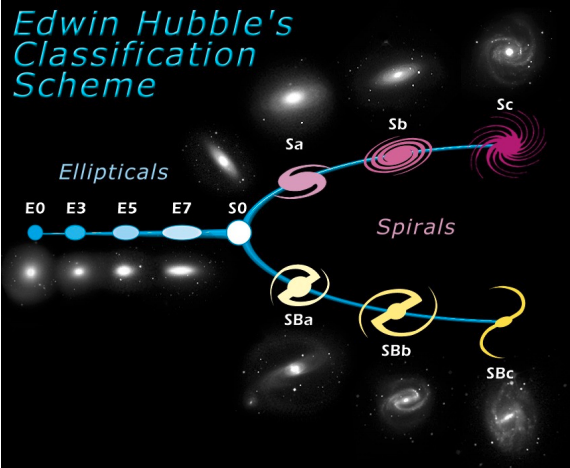
\includegraphics[width=0.75\textwidth]{figs/Screen Shot 2021-08-27 at 1.35.32 PM.png}
    \caption{Hubble Classification Scheme}
    \label{fig:hub_scheme}
\end{figure}

There have been others developed since then, suhc as the deVaucouleur system or the T-type system. 

\begin{figure}[ht!]
    \centering
    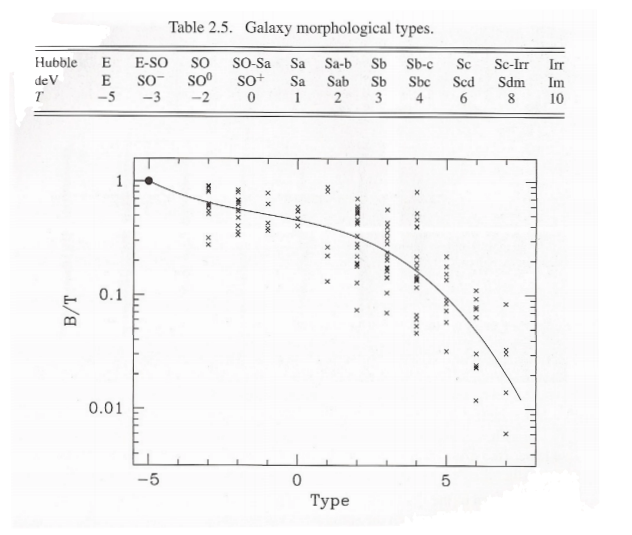
\includegraphics[width=0.75\textwidth]{figs/Screen Shot 2021-08-27 at 1.37.01 PM.png}
    \caption{Other classification schemes. }
    \label{fig:other_schemes}
\end{figure}

Recently, we have started a \textbf{newer, fresher} classification based on rotation! 

\begin{figure}[ht!]
    \centering
    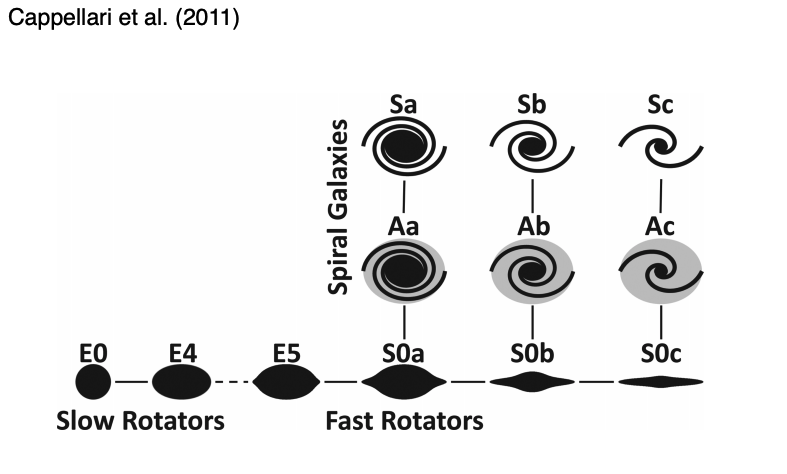
\includegraphics[width=0.75\textwidth]{figs/Screen Shot 2021-08-27 at 1.38.11 PM.png}
    \caption{Fast and slow rotation scheme. }
    \label{fig:fast_slow_rot}
\end{figure}

There are some difficulties in determined morphology, though:
\begin{itemize}
    \item It depends on orientation.
    \item It depends on wavelength. 
    \item Subjective.
    \item etc.
\end{itemize}



\section{August 27, 2021: Global Properties and Galaxy Correlations}

\subsection{Morpohology, Continued}

Let's start by looking a little deeper at the morphological classifications from last time. First, let's look at spectra along the Hubble sequence, HI content, stellar mass, stellar surface density, oxygen abundance, and environment. The results are presented in Figures 4 through 7.

\begin{figure}%
    \centering
    \subfloat[\centering ]{{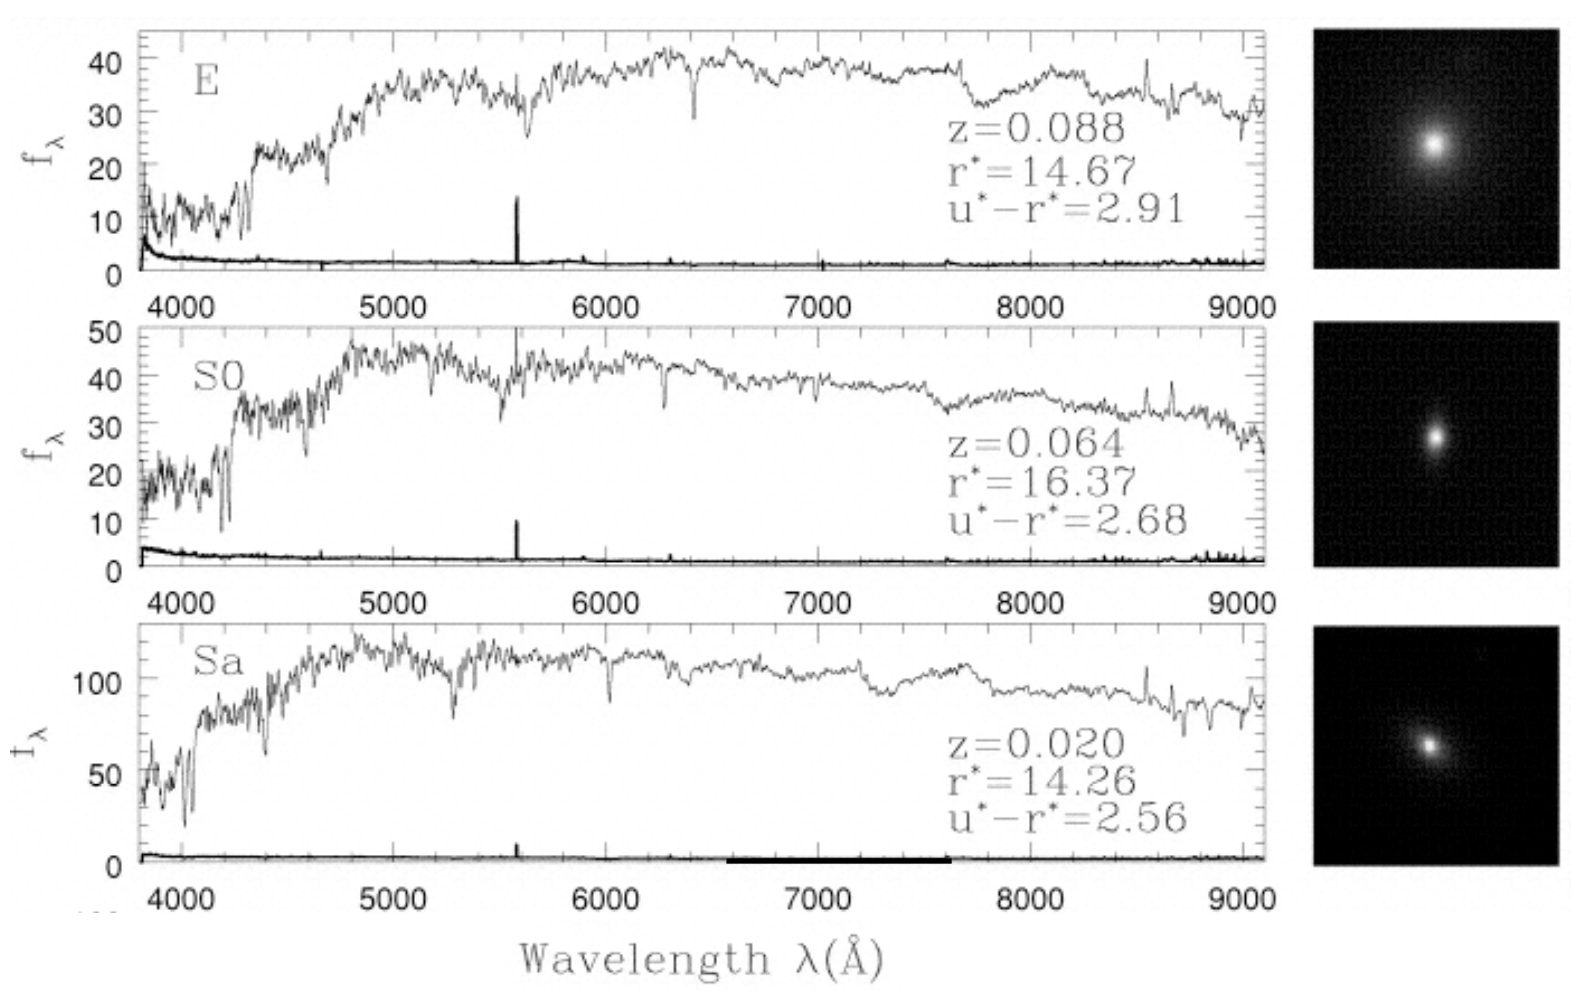
\includegraphics[width=7.5cm]{figs/Screen Shot 2021-08-27 at 1.44.05 PM.png} }}%
    \qquad
    \subfloat[\centering]{{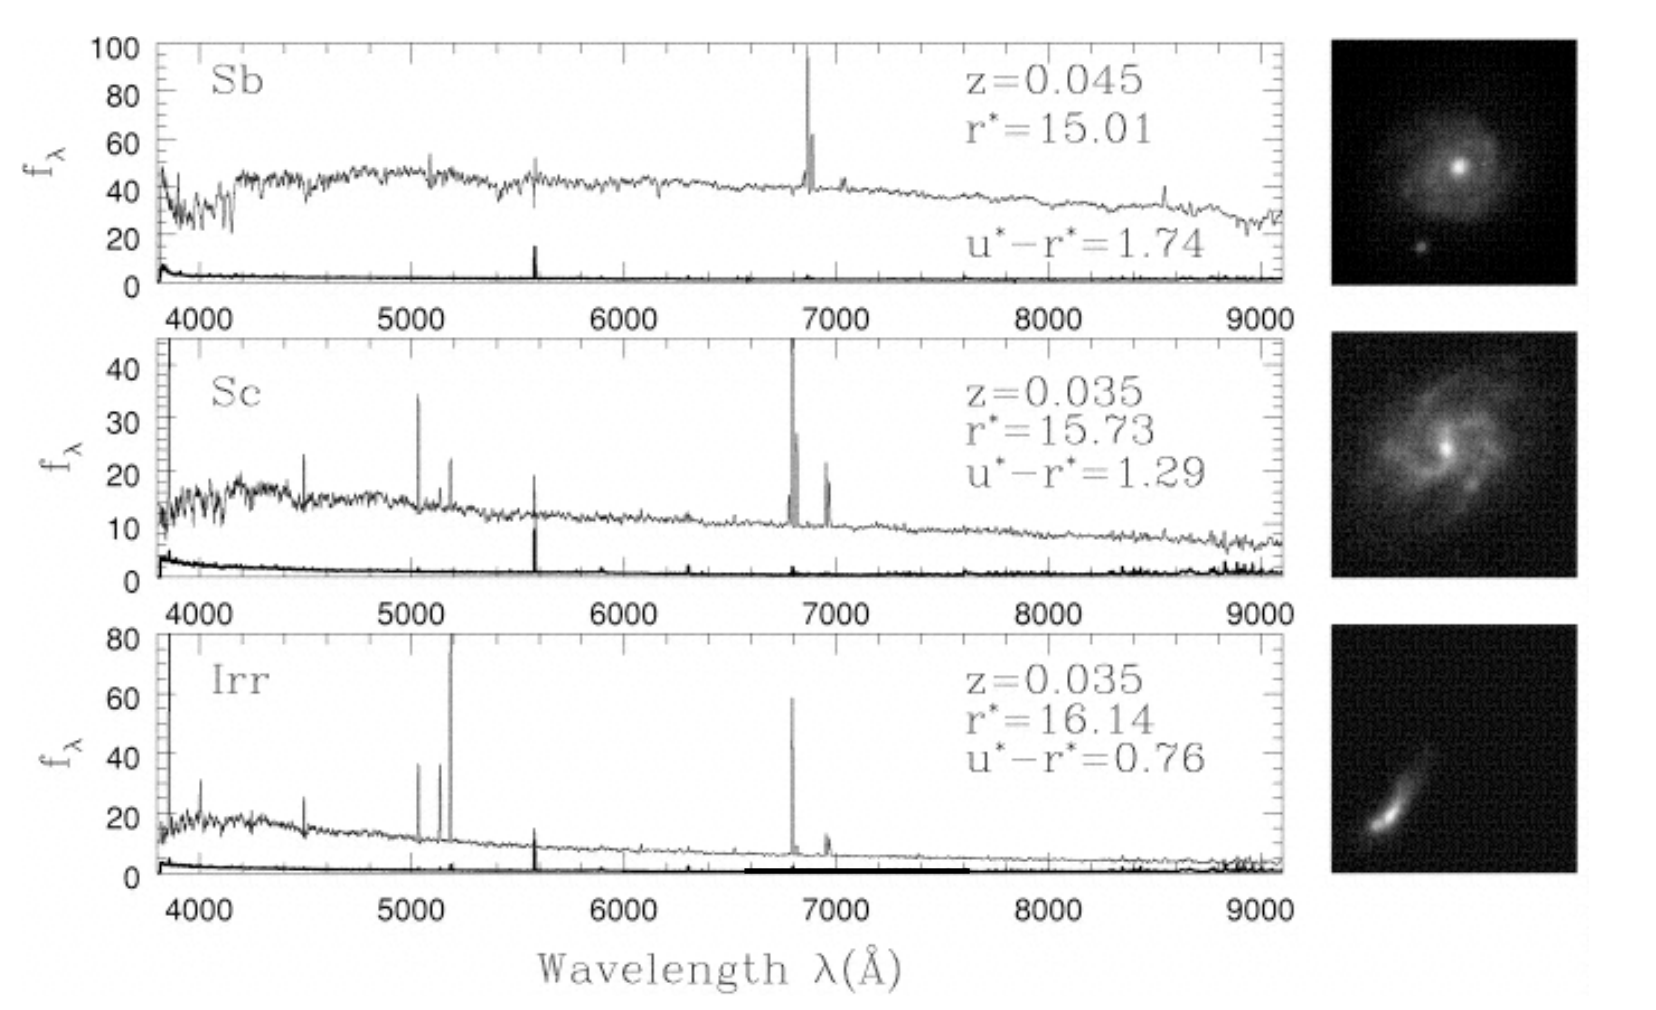
\includegraphics[width=7.5cm]{figs/Screen Shot 2021-08-27 at 1.44.15 PM.png} }}%
    \caption{Spectra along the Hubble sequence. Early type galaxies are much redder and have deeper absorption features. Later-type galaxies have spectra that are dominated by emission from hot stars. }%
    \label{fig:spec_types}%
\end{figure}

\begin{figure}[ht!]
    \centering
    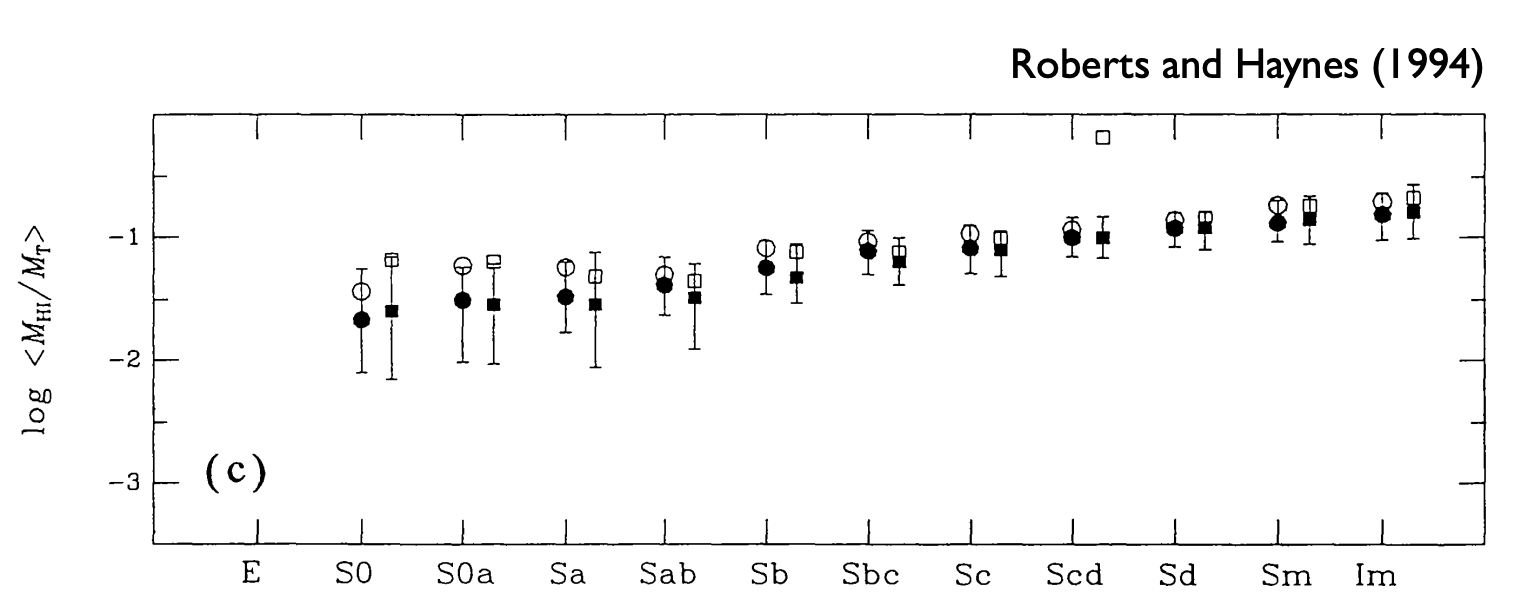
\includegraphics[width=0.75\textwidth]{figs/Screen Shot 2021-08-27 at 1.44.29 PM.png}
    \caption{HI content as a function of morphology.}
    \label{fig:HI_conte}
\end{figure}

\begin{figure}[ht!]
    \centering
    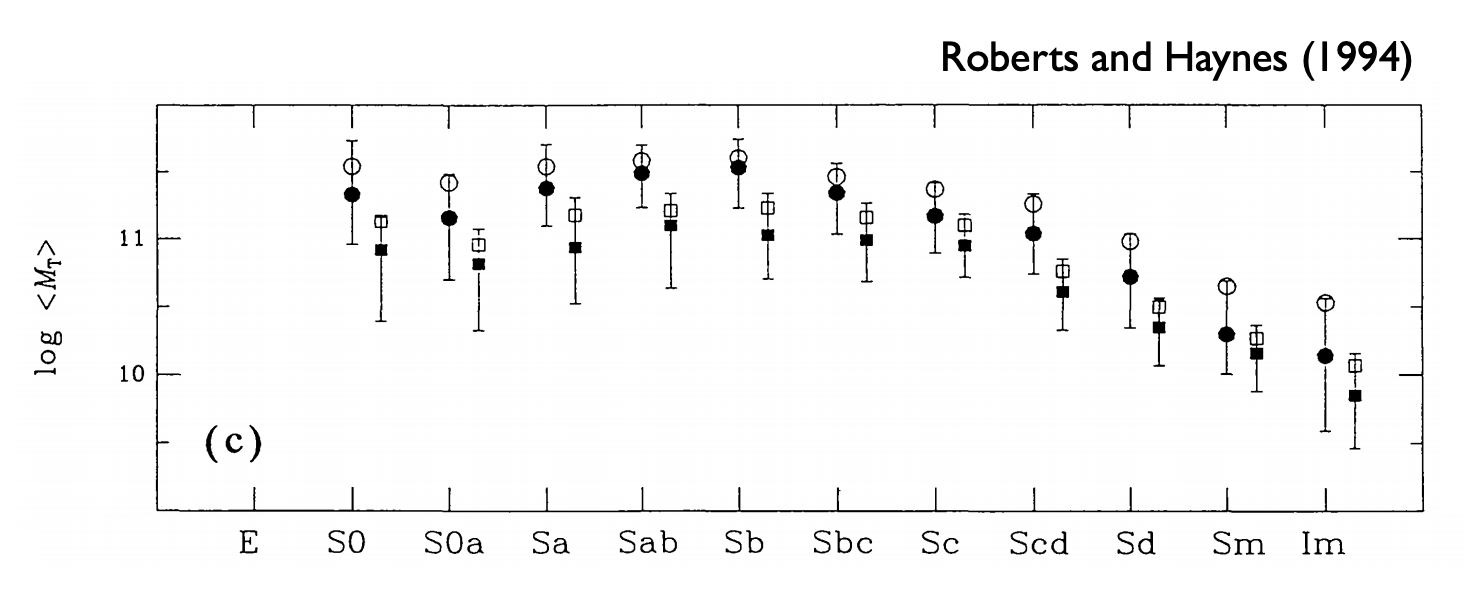
\includegraphics[width=0.75\textwidth]{figs/Screen Shot 2021-08-27 at 1.44.38 PM.png}
    \caption{Total stellar mass as a function of morphology. }
    \label{fig:to_mas}
\end{figure}

\begin{figure}[ht!]
    \centering
    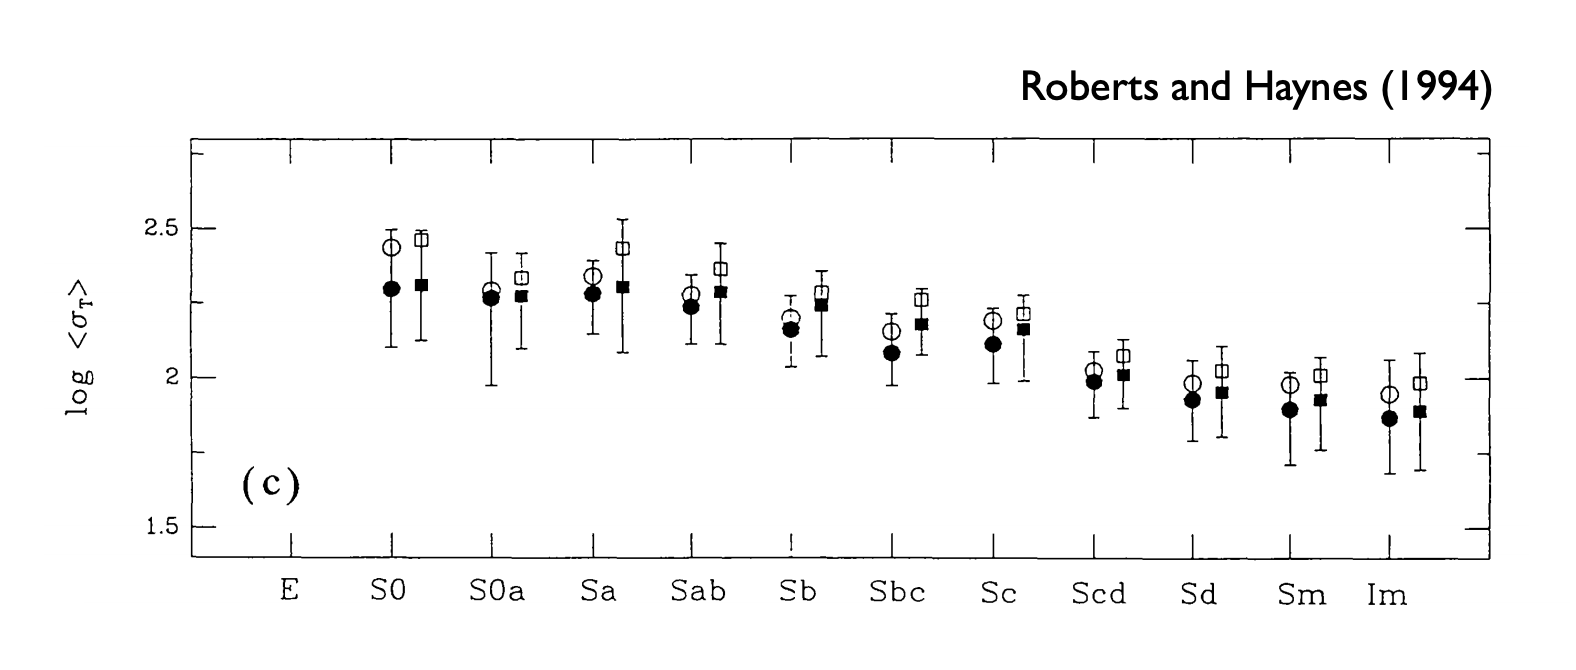
\includegraphics[width=0.75\textwidth]{figs/Screen Shot 2021-08-27 at 1.44.48 PM.png}
    \caption{Stellar surface density as a function of morphology.}
    \label{fig:surf_dens}
\end{figure}

\begin{figure}[ht!]
    \centering
    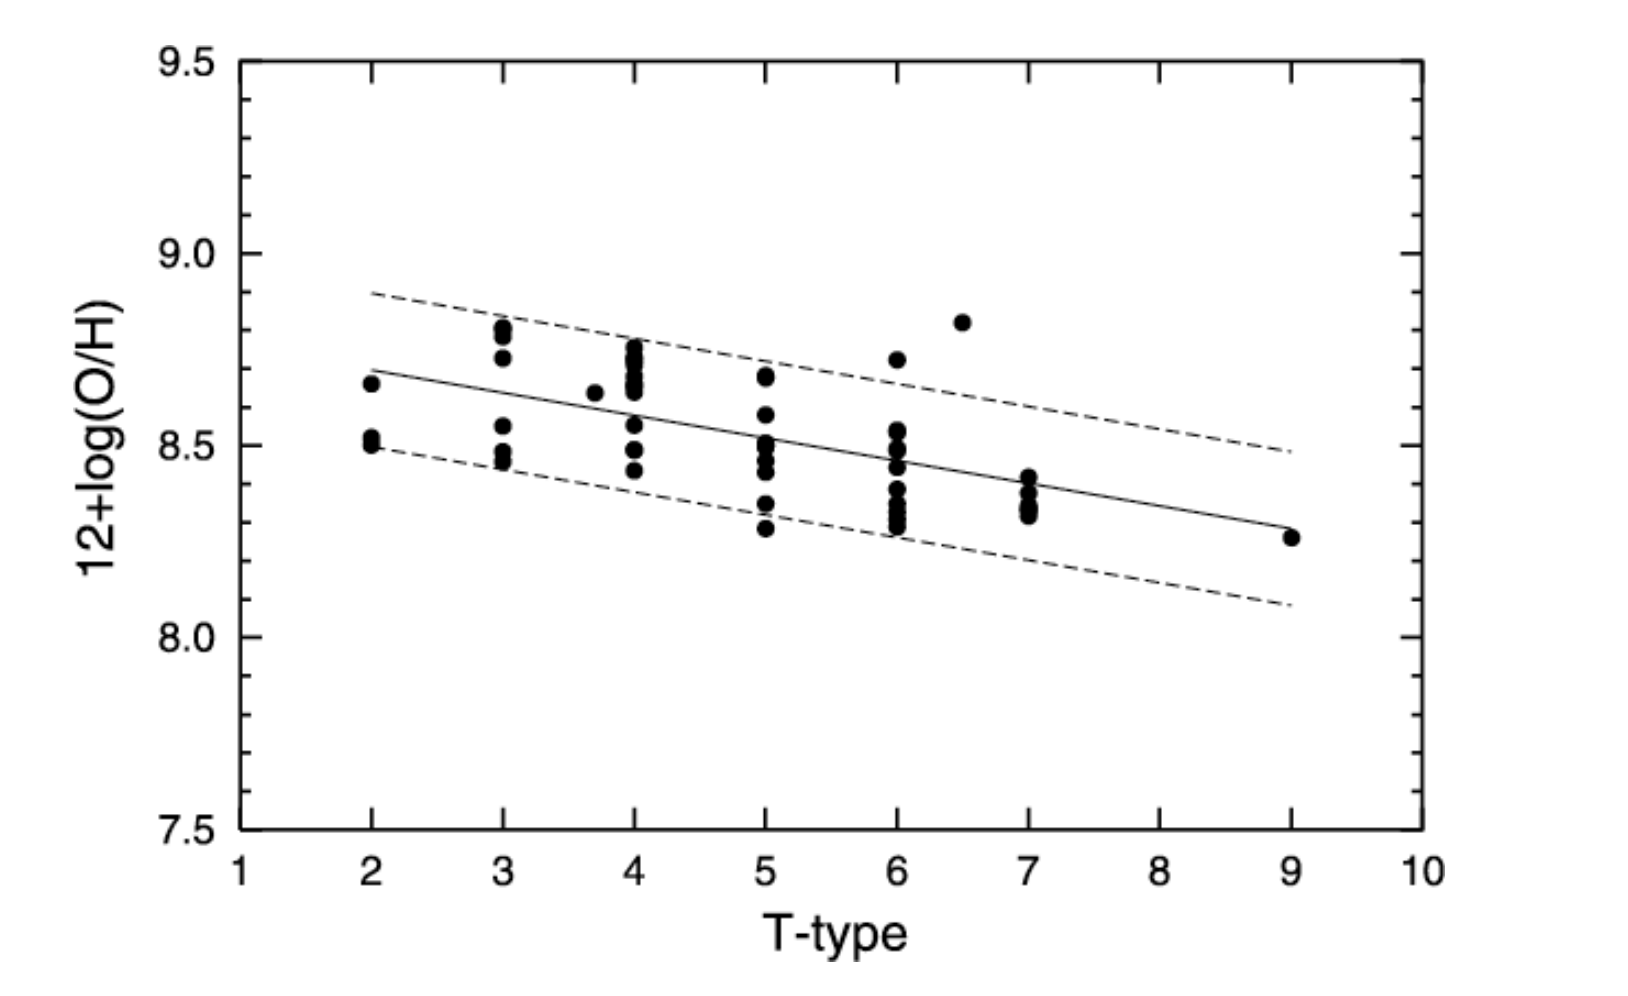
\includegraphics[width=0.75\textwidth]{figs/Screen Shot 2021-08-27 at 1.44.59 PM.png}
    \caption{Oxygen abundance as a function of morphology. Note that the $+12$ is just to make things positive!}
    \label{fig:oxy}
\end{figure}


Here are the general trends. Star formation rate, gas fractions, and rotational support increase for later-type galaxies. Mass, metallicity, environment, and mass surface density increase for earlier-type galaxies. 

\subsection{Units and Quantities}

Let's do a quick review of units and other quantities we will use through the semester. Recall \textbf{specific intensity}:

\begin{equation}
    \boxed{[I_\nu] = \frac{\unit{ergs}}{\unit{s} \unit{cm}^2 \unit{sr} \unit{Hz}}}
\end{equation}

We also have the quantity of \textbf{flux density}:
\begin{equation}
    \boxed{[F_\lambda] = \frac{\unit{ergs}}{\unit{s} \unit{cm}^2 \A}}
\end{equation}

In general, remember that $F_\lambda \neq F_\nu$. Instead, $F_\lambda \mathrm{d}\lambda = F_\nu \mathrm{d}\nu$, and thus:

\begin{equation}
    F_\nu = \frac{c}{\nu^2}F_\lambda
\end{equation}

We also discussed magnitudes which are a terrible unit. But alas, we must use them. The apparent magnitude is defined as:

\begin{equation}
    m_x = -2.5\log_{10}\left(\frac{F_x}{F_{x,0}}\right)
\end{equation}

where the subscript $x$ represents a filter and $F_{x,0}$ is the flux of a reference in filter $x$. Historically, stellar astronomers have used Vega as the reference point. Galactic astronomers have used AB magnitudes (I have no idea what the reference is, here). In this \textbf{AB Mangnitude system}, we have:

\begin{equation}
    \boxed{m_x = -2.5\log_{10}\left(F_x\right) - 48.57}
\end{equation}

\textbf{Absolute magnitudes} are defined as:

\begin{equation}
    \boxed{\underbrace{m_x - M_x}_{\text{distance modulus }\mu} =  5\log_{10}\left(\frac{d}{d_{0}}\right)\text{, where } d_0 \equiv 10 \pc}
\end{equation}

We also need to be familiar with redshift, both due to expansion and relativistic velocities. We define the redshift $z$:

\begin{equation}
    \boxed{1+z = \frac{\lambda_{obs}}{\lambda_{em}}}
\end{equation}

In the case of particles moving at relativistic speeds, we have:

\begin{equation}
    1+z = \sqrt{\frac{1+v/c}{1-v/c}}
\end{equation}

In the non-relativistic case, we have the \textbf{Hubble's Law}:

\begin{equation}
    v \approx cz
\end{equation}

Lastly, we defined the \textbf{luminosity distance} as:

\begin{equation}
    d_L^2 \equiv \frac{L}{4\pi F}
\end{equation}

\subsection{Sloan Digital Sky Survey}

The Sloand Digital Sky Survey (SDSS) revolutionized astronomy. Not only did it take spectra and photometry of millions of galaxies, but it also redefined the photometric system from the Johnson-Cousins system to the familiar \textit{ugriz} system. First, let's discuss an important aspect of filters: \textbf{filter response functions}. This is basically like a sensitivity/efficiency, and these curves look like this: 

\begin{figure}
    \centering
    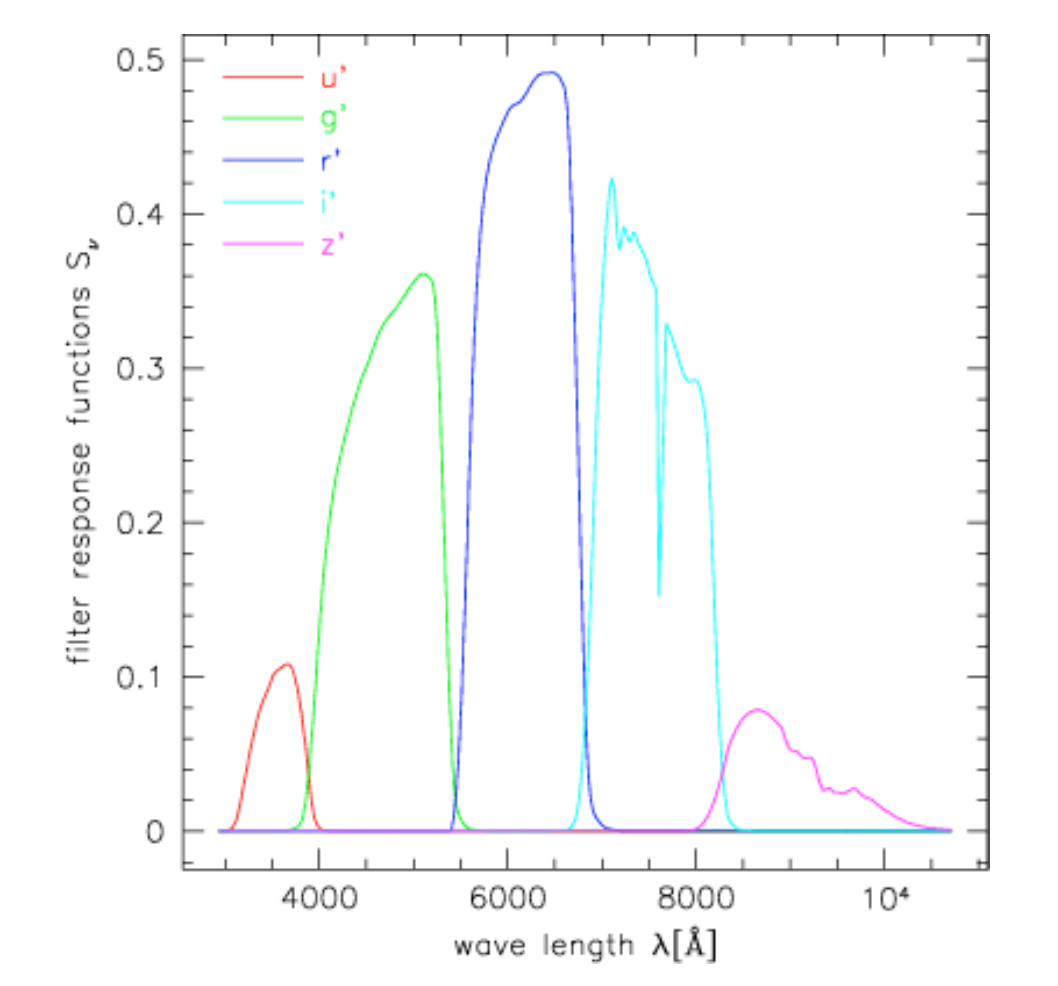
\includegraphics[width=0.75\textwidth]{figs/Screen Shot 2021-08-27 at 2.12.21 PM.png}
    \caption{SDSS transmission curves.}
    \label{fig:trans_curves}
\end{figure}

Note that:

\begin{equation}
    F_x = \frac{\int_0^{\infty} S_\nu F_\nu \,\mathrm{d}\nu}{\int_0^{\infty} S_\nu \mathrm{d}\nu}
\end{equation}

SDSS had 5 band photometry for millions of objects, which means we need to look at spectral energy distributions (SEDs). These are basically low resolution spectra, but we can still learn a ton from these plots! We can match SEDs to synthetic galaxy spectra to measure photometric redshift or learn about broad properties of the galaxies. 

\begin{figure}
    \centering
    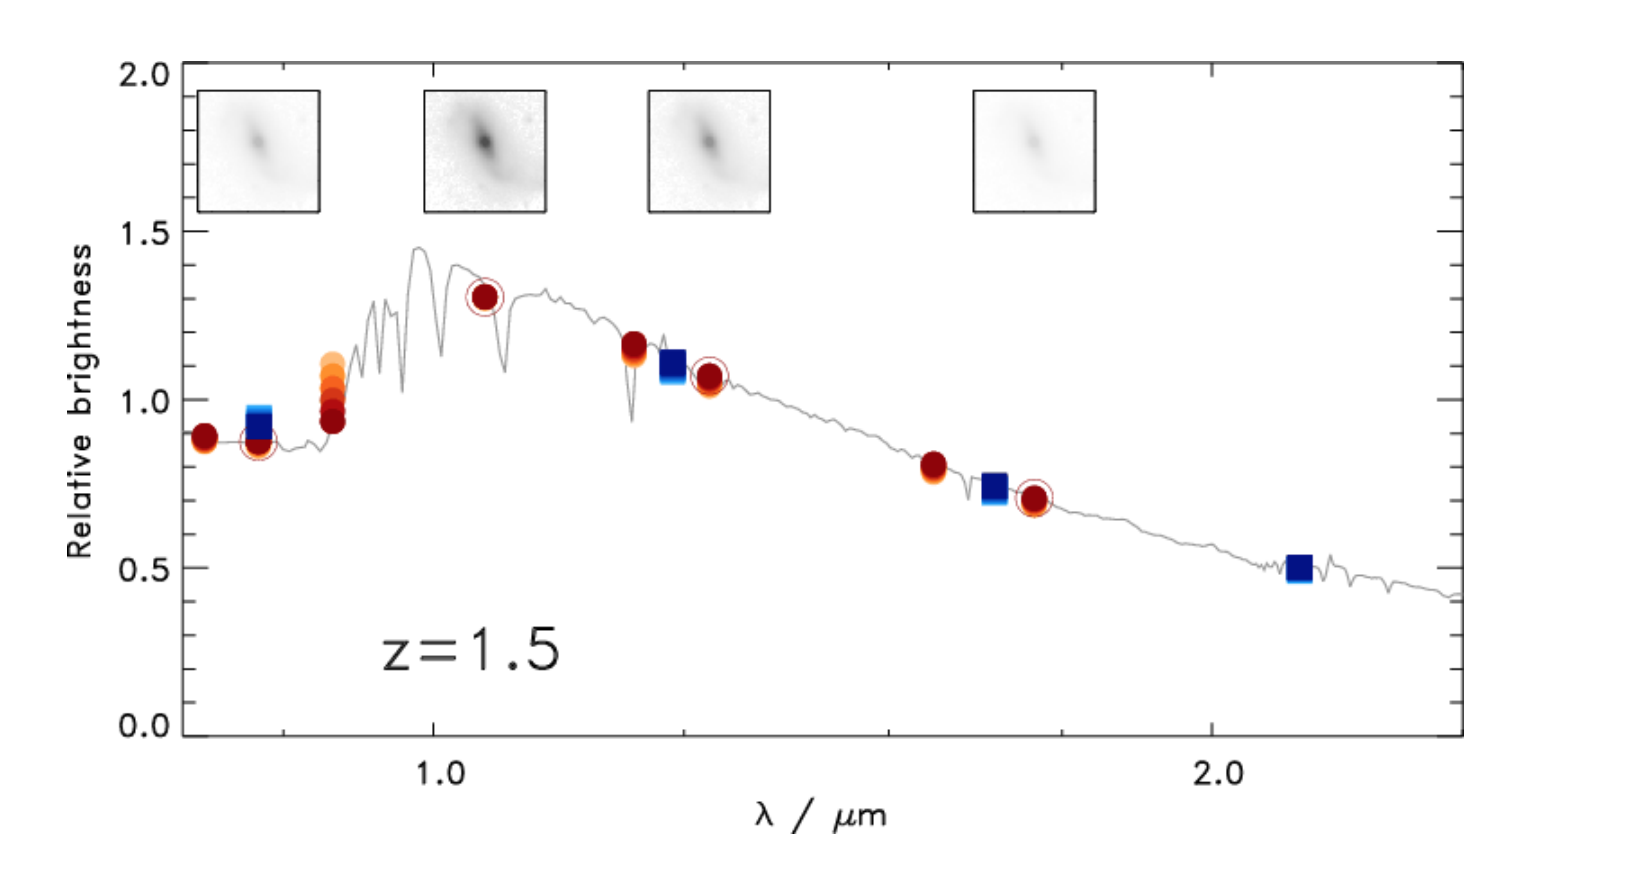
\includegraphics[width=0.75\textwidth]{figs/Screen Shot 2021-08-27 at 2.25.14 PM.png}
    \caption{Example SED with fit for photometric redshift. }
    \label{fig:synth_fit}
\end{figure}

\begin{figure}
    \centering
    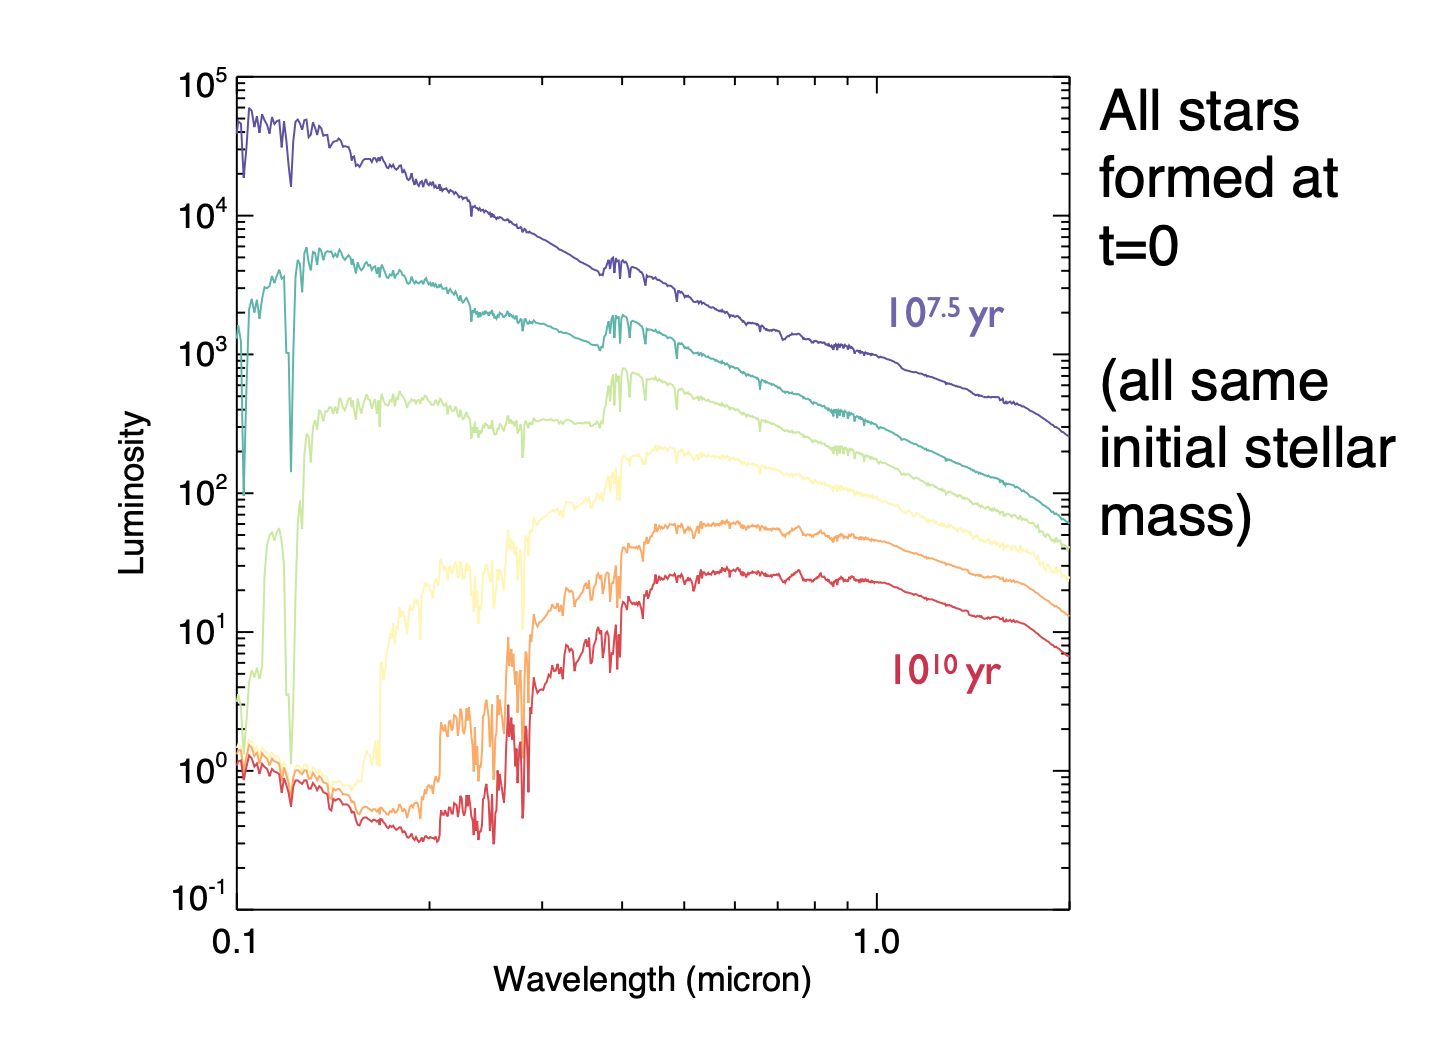
\includegraphics[width=0.75\textwidth]{figs/Screen Shot 2021-08-27 at 2.24.29 PM.png}
    \caption{Synthetic galaxy spectra as a function of age. }
    \label{fig:synth_spec}
\end{figure}

One thing to note is that redder galaxies are less luminous for the same stellar mass, as we can see in the synthetic spectra. This result in redder galaxies having higher mass to light ratios! 

\subsection{K Corrections}

Here's a figure to demonstrate K-corrections.

\begin{figure}
    \centering
    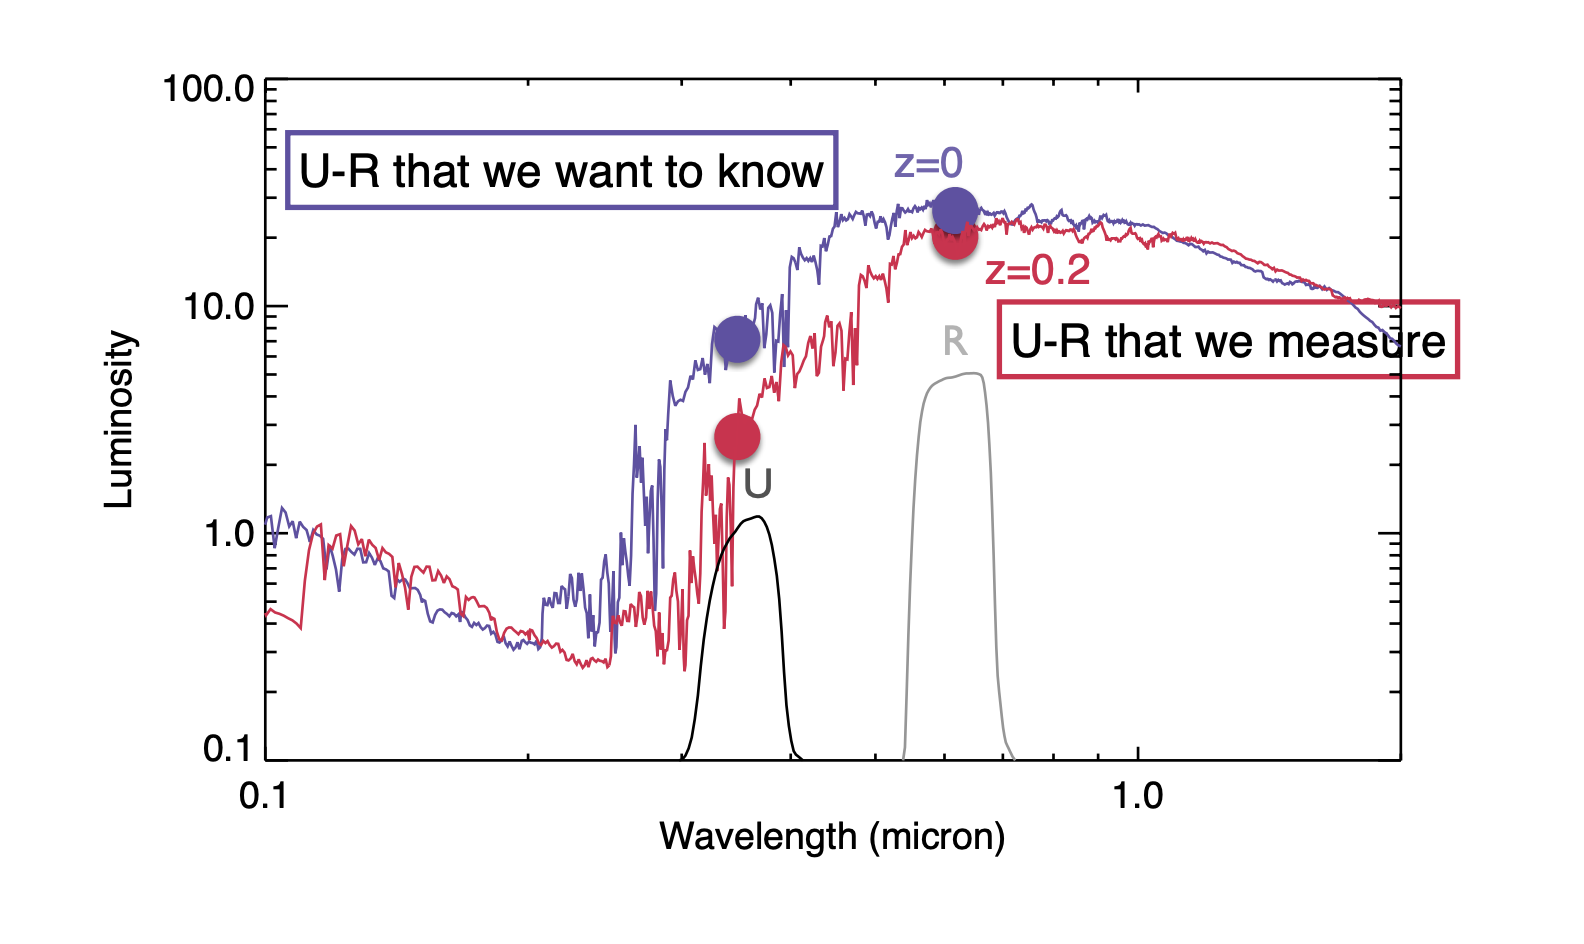
\includegraphics[width=0.75\textwidth]{figs/Screen Shot 2021-08-27 at 2.27.30 PM.png}
    \caption{The SED changes as a function of redshift. We ultimately want the rest-frame $u-r$ value, but we need to correct the observed spectrum in some way since $u-r$ itself is a function of redshift. This is the concept of a $K$ correction. }
    \label{fig:k_correc}
\end{figure}

We model $K$ corrections in this way:

\begin{equation}
    m = M + \mu + K
\end{equation}
\begin{equation}
    \text{observed} = \text{intrinsic} + \text{distance} + \text{expansion}
\end{equation}

\subsection{Trends of Stellar Mass with Color}

\begin{figure}
    \centering
    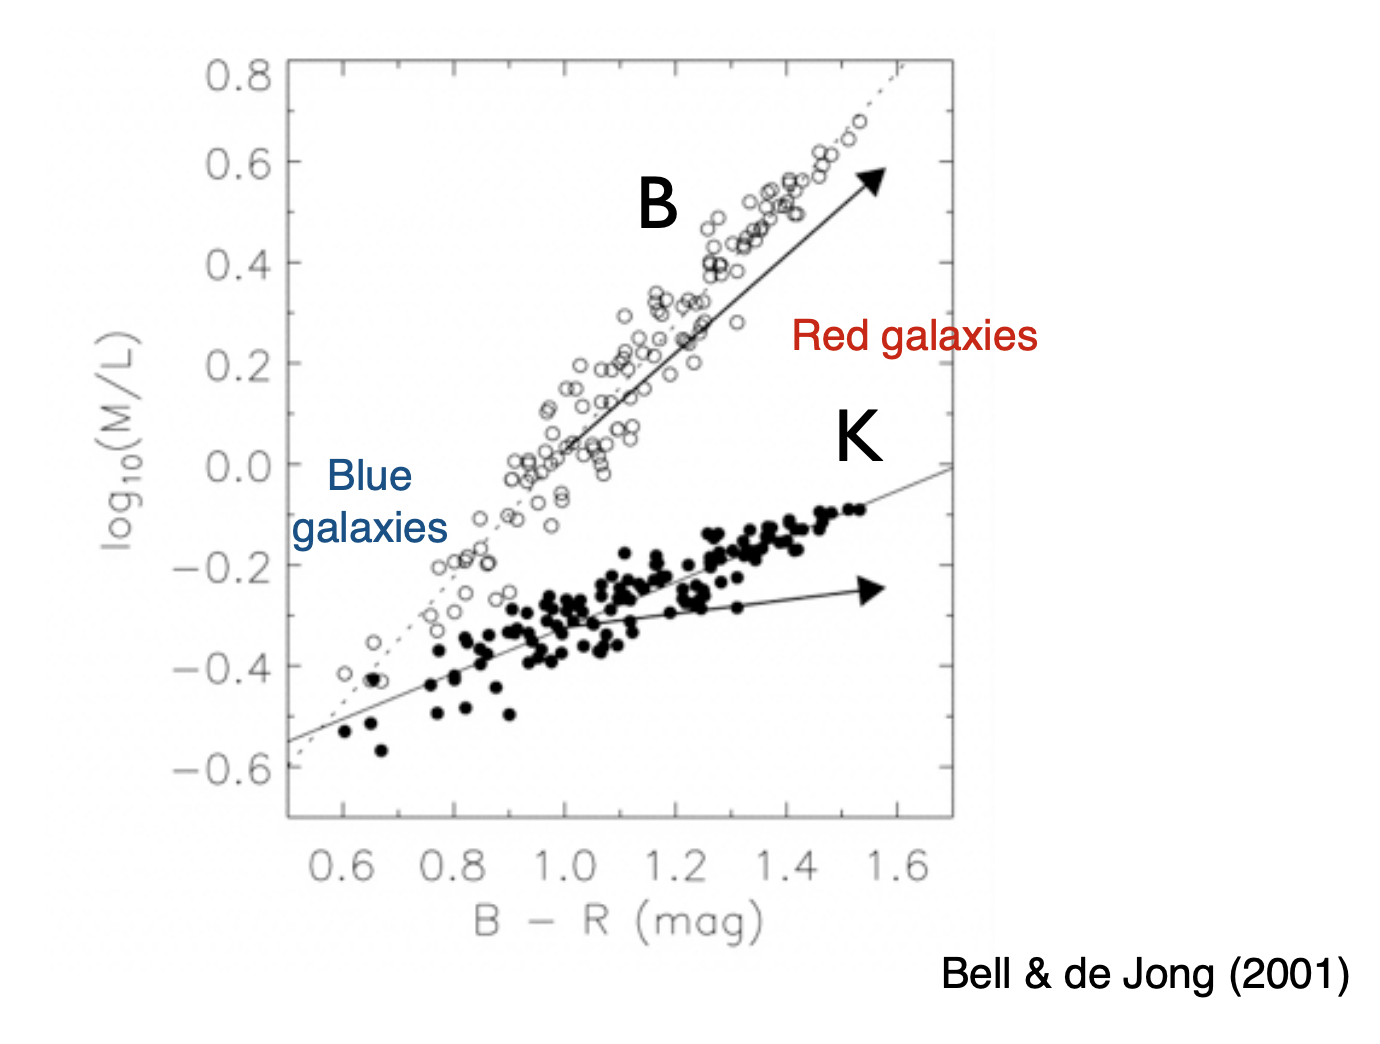
\includegraphics[width=0.75\textwidth]{figs/Screen Shot 2021-08-27 at 2.31.11 PM.png}
    \caption{Trends of stellar mass to light ratio with color. }
    \label{fig:color_ml}
\end{figure}

\begin{figure}
    \centering
    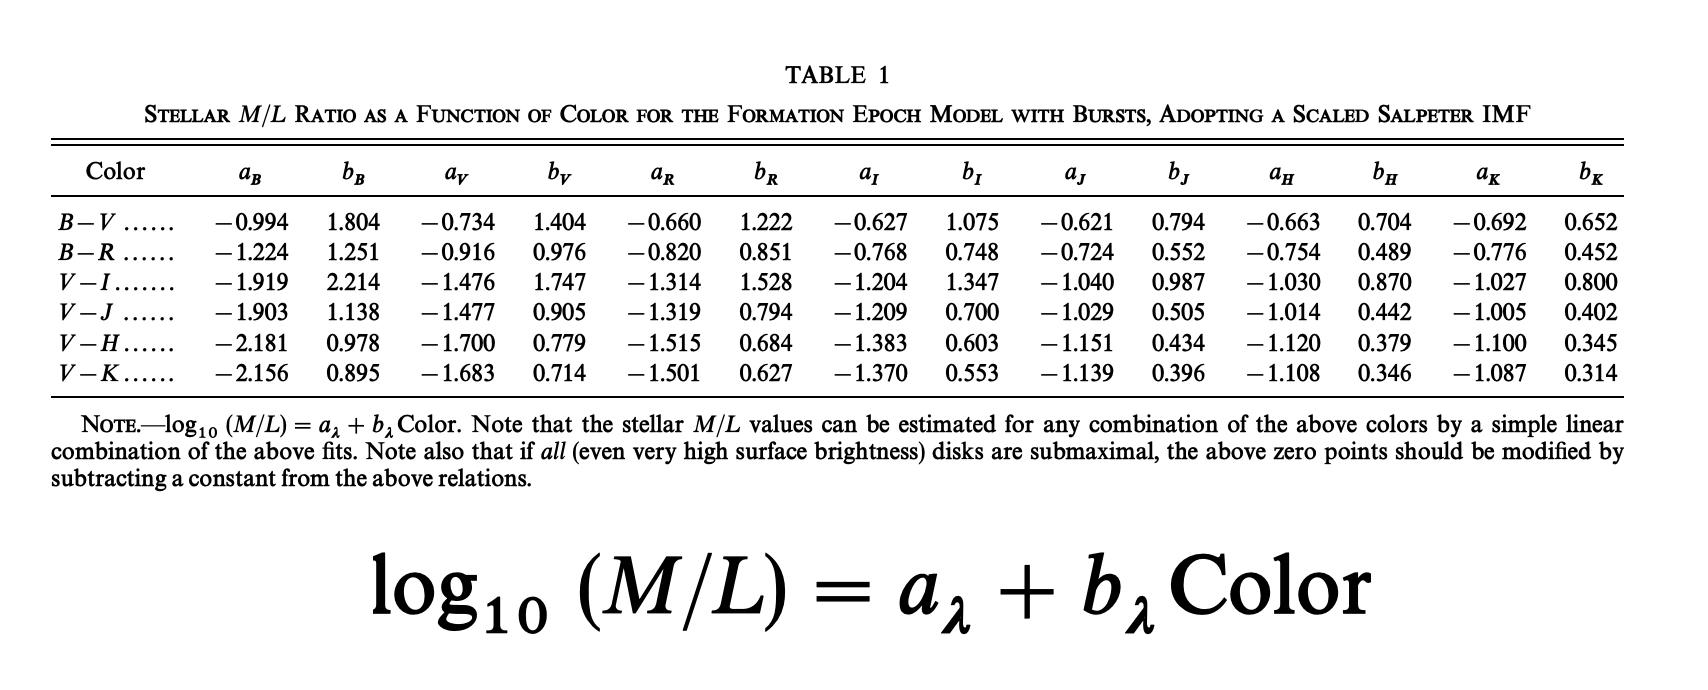
\includegraphics[width=0.75\textwidth]{figs/Screen Shot 2021-08-27 at 2.31.21 PM.png}
    \caption{Table which was a first attempt at quantifying this relationship. Much better ways of doing this now!}
    \label{fig:color_ml_2}
\end{figure}

\section{September 1, 2021: Global Properties and Galaxy Correlations}

\subsection{AB Magnitudes and Vega Magnitudes}

The AB magntiude system is the \textbf{absolute} system. 

\begin{equation}
    m_{AB} = -2.5\log_{10}\left(\frac{f_\nu}{3631 \jy }\right) = -2.5\log_{10}\left(f_\nu\right) - 48.57
\end{equation}

We have a differ net system called the \textbf{STmag}, which is similar but in wavelength; not in frequency. The conversion between the two is non-trivial. The corrections in the optical are small, but these increase at larger and smaller wavelengths. 

\subsection{Synthetic galaxy spectra as a function of age}

This discussion primarily revolves around Figure 11, the figure of the synthetic spectra as a function of age. Make sure to be able to re-create this type of plot!

Imagine taking a stellar population synthesis model at the same time, with some mass. Young populations are brighter per unit mass, and they are bluer. Redder galaxies have higher mass to light ratios. 

Let's now move onto K-corrections...

\subsection{K-corrections}

The idea: Normally we observe through filters, meaning over some specific $\mathrm{d}\lambda$. For a typical galaxy spectra at $z=0$:

\begin{equation}
    L = \int_{\lambda_1}^{\lambda_2} f(\lambda) \mathrm{d}\lambda 
\end{equation}

Due to redshift effects, the light emitted gets shifted by a factor of $(1+z)$. Looking at galaxies at higher $z$, we receive emission from shorter wavelengths at a slower rate. Knowing the spectra shape, we can correct for this via K-correction. The \textbf{assumption: we know something about the intrinsic spectrum.} Here's a figure explaining what we mean:

\begin{figure}[h]
    \centering
    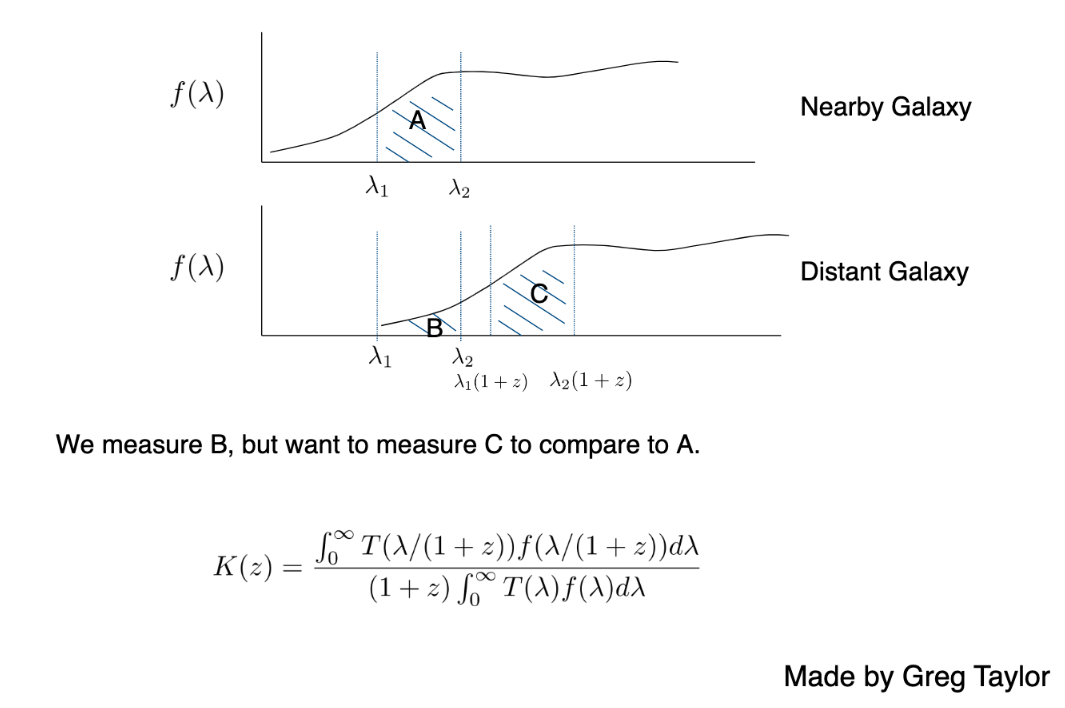
\includegraphics[width=0.75\textwidth]{figs/Screen Shot 2021-09-02 at 9.40.32 AM.png}
    \caption{K-corrections, by Greg Taylor.}
    \label{fig:kcorr}
\end{figure}

Here's a derivation:

The flux we observe per unit wavelength, $F_\lambda$ (the emitted luminosity is: $L_{\lambda/(1+z)}$):

\begin{equation}
    F_\lambda = \frac{1}{1+z} \frac{L_{\lambda/(1+z)}}{4\pi D_L^2} = \frac{1}{1+z}\frac{L_{\lambda/(1+z)}}{L_\lambda} \frac{L_\lambda}{4\pi D_L^2}
\end{equation}

Equivalently: $F_\nu \propto (1+z)$. After some work, we can see that:

\be
    m = M + \mu + K, \text{ where } K \equiv -2.5\log_{10}\left(F_\lambda\right)
\ee

Generally, $K$ corrections are positive. There are unusual cases where the $K$ correction is negative, but that's uncommon. 

\subsection{Stellar Masses (Bell \& de Jong 2001)}

\begin{figure}[h!]
    \centering
    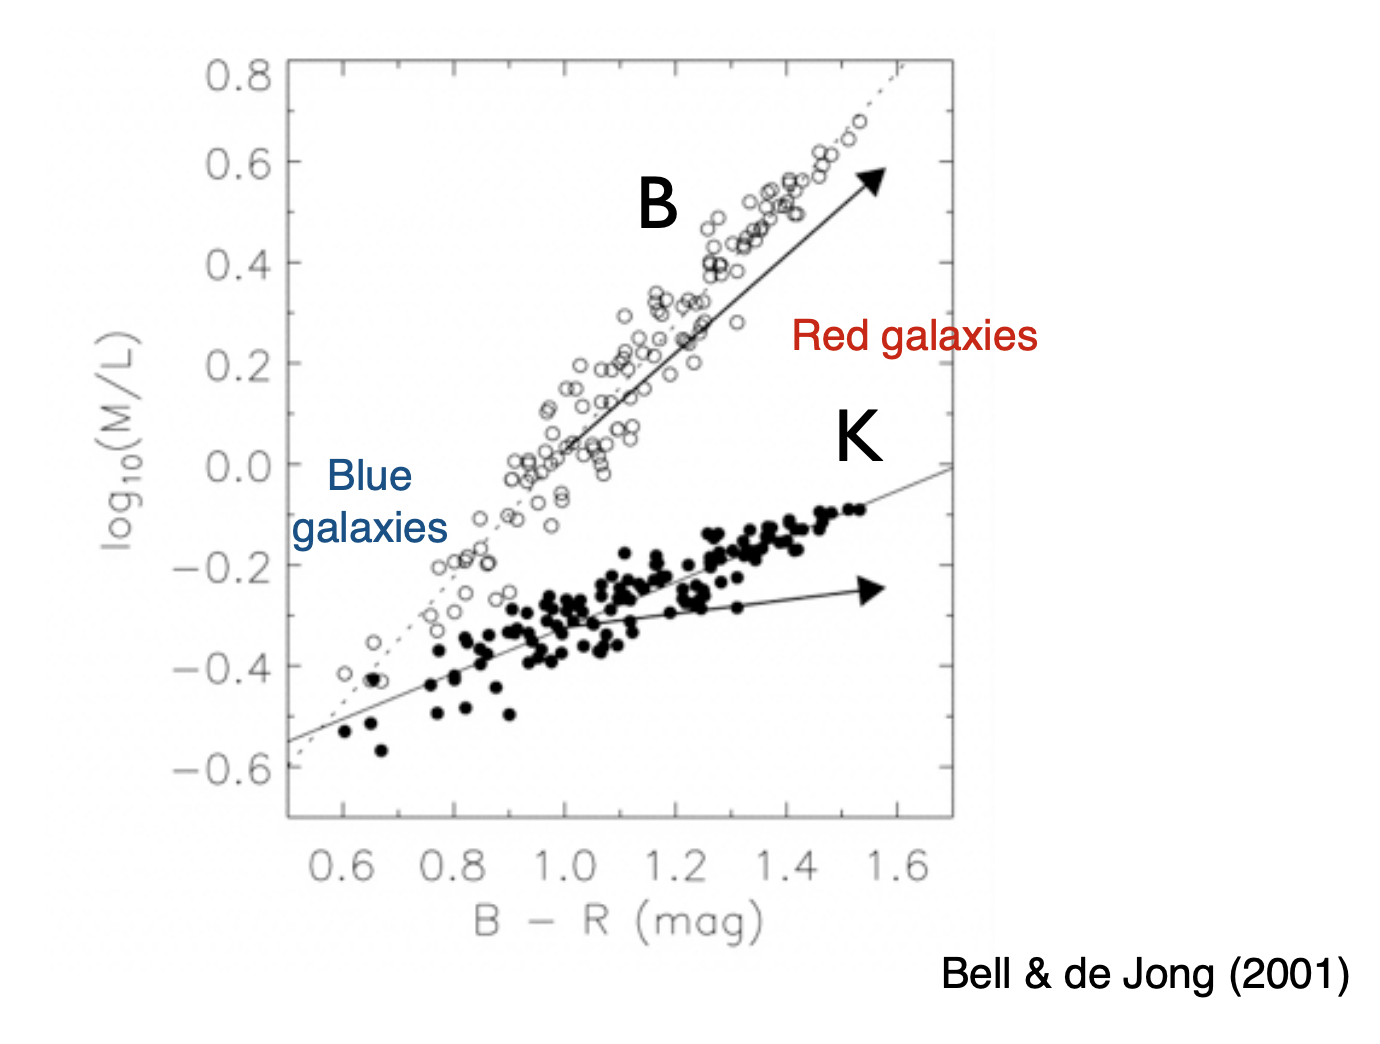
\includegraphics[width=0.75\textwidth]{figs/Screen Shot 2021-08-27 at 2.31.11 PM.png}
    \caption{Re-visited on September 1!}
    \label{fig:color_ml_21}
\end{figure}

We're discussing the figure here. The x-axis is the $B-R$ color, and the y-axis is the inferred mass-to-light ratio. Each dot is an individual galaxy. The two groups are $B$ and $K$ band mass to light ratios, with the key takeaway is that \textbf{there is no one-to-one mapping between mass and luminosity}. Instead, luminosity \textbf{and color} can give you a mass. 

It's best to observe $K$ band for measuring mass to light ratios so that the spectrum isn't dominated by \textbf{single O stars}. The ideal case is a filter for which the mass-to-light does not depend on the color. $K$ is close, but it's not ideal! 

However, bluer colors are better at disentangling the age of a stellar population. 

\subsection{SEDs for Different Metallicities}

Here's an interesting figure:

\begin{figure}
    \centering
    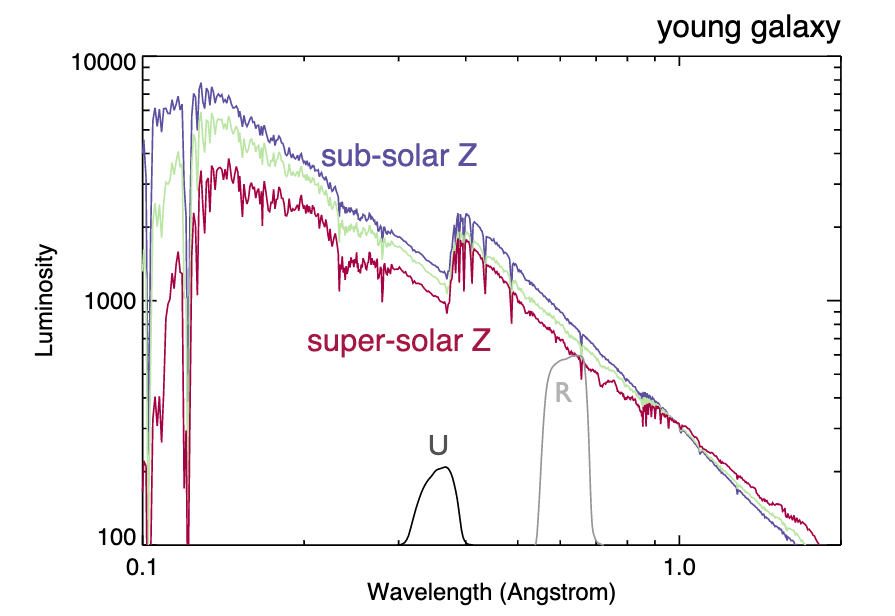
\includegraphics[width=0.66\textwidth]{figs/Screen Shot 2021-09-02 at 9.41.22 AM.png}
    \caption{SEDs for different metallicities for a young galaxy. What are the takeaways? }
    \label{fig:sed_z}
\end{figure}

For a fixed mass and galaxy type, lower-metallicities are brighter, particularly in the blue! As you go to the red end of the spectrum, the SEDs blend together better. 

This is due to \textbf{opacity}. Fewer metallicites have a lower opacity, and so more light gets out. For higher metallicities, we have a higher opacity and thus less light gets out. 

Also know that the age has a huge impact on the spectra, but metallicity has much less of an effect. This also means that metallicity is harder to measure than age. They're also \textbf{degenerate} with each other. 

\begin{figure}
    \centering
    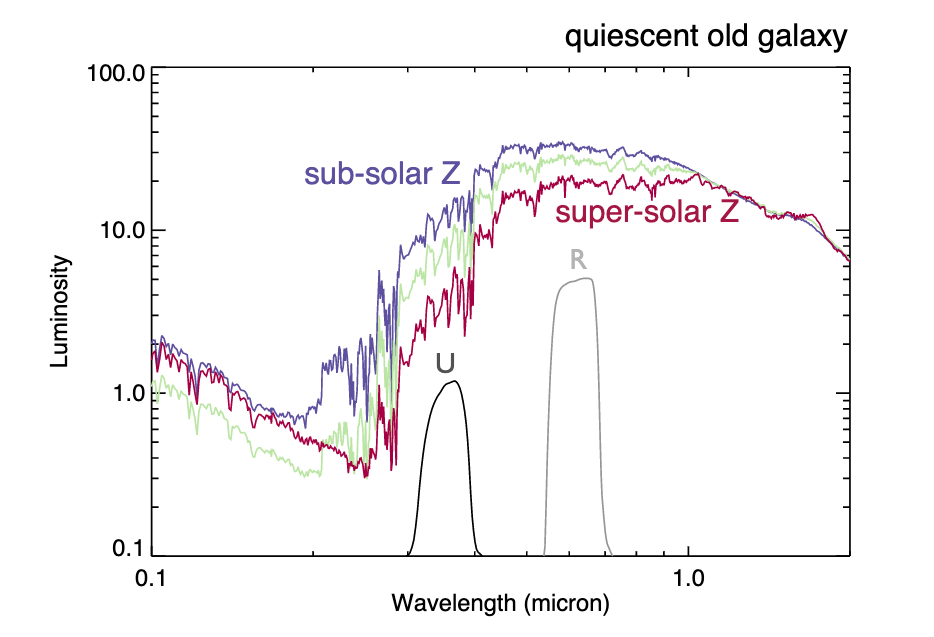
\includegraphics[width=0.66\textwidth]{figs/Screen Shot 2021-09-02 at 9.41.34 AM.png}
    \caption{SEDs for different metallicities for an old galaxy. What are the takeaways? }
    \label{fig:sed_z_old}
\end{figure}

What's different for the older, quiescient galaxy? At the blue end of the spectrum, solar metallicity populations are actually \textbf{weakest}! Detailed stellar physics of post-main sequence stars dictate this effect. 

\subsection{Color Sequences}

Let's look at color vs. stellar mass of galaxies. The color of the galaxy $m_u - m_r$ can be thought of as the slope of the SED. Interpreted differently, this is:

\begin{equation}
    u -r = -2.5\log_{10}(F_u) + 2.5\log_{10}(F_r) \rightarrow \boxed{u-r = -2.5\log_{10}\left(\frac{F_u}{F_R}\right)}
\end{equation}

Here's a cool plot:

\begin{figure}
    \centering
    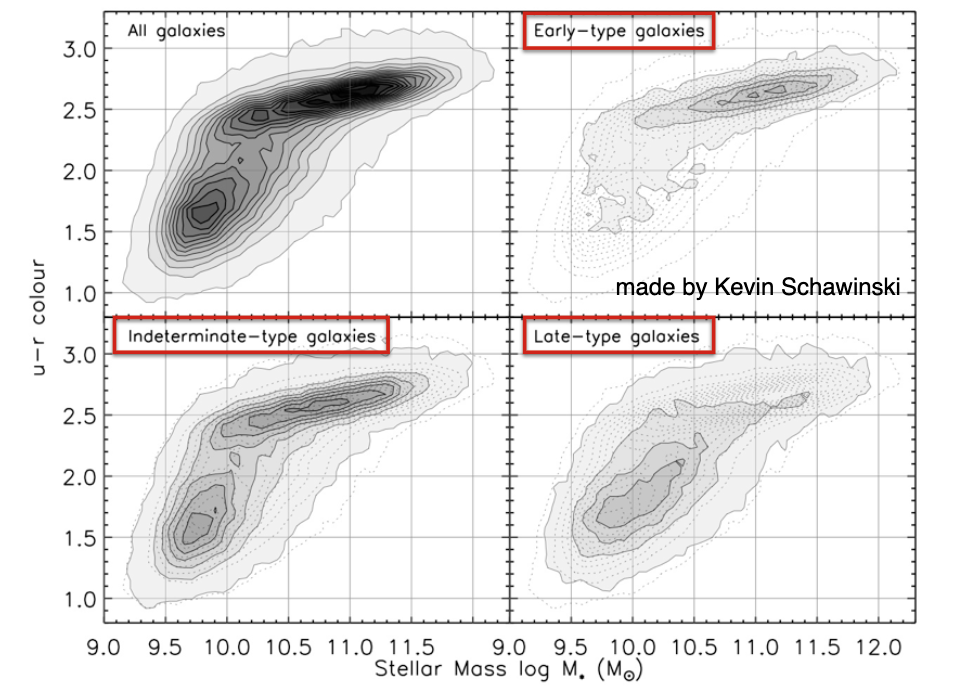
\includegraphics[width=0.66\textwidth]{figs/Screen Shot 2021-09-02 at 9.41.59 AM.png}
    \caption{Color sequences. Note that there are two pileups: redder and more massive; blue and less massive.}
    \label{fig:color_sequences}
\end{figure}

If you measure a galaxy color, we can measure the mass to light ratio. \textbf{This is a key reason to measure color.} If we also measure the spectrum (or the SED with multi-band photometry), we can get the galaxy flux, redshift, and make a K-correction. Note we can also measure the mass-to-light (or mass) from the SED, too! 

What are some other trends in this plot? The early-type galaxies hardly change in color but increase 2 dex in mass. This 

\subsection{Galaxy Correlations in the SDSS}

Let's talk about the D-4000 decrement from Kauffman et al., 2003:

\begin{figure}
    \centering
    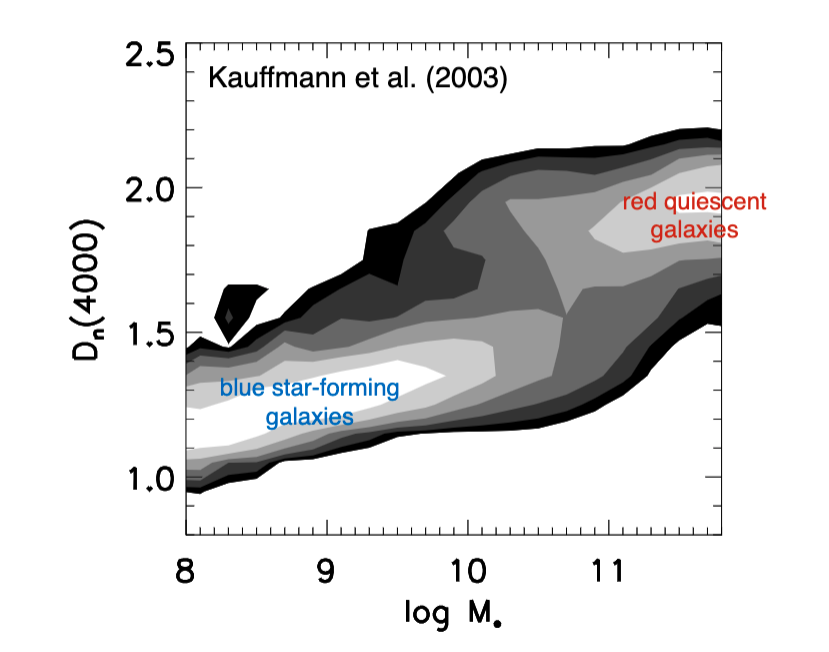
\includegraphics[width=0.66\textwidth]{figs/Screen Shot 2021-09-02 at 9.42.37 AM.png}
    \caption{We can see that the D4000 feature very nicely separates the red, quiescient galaxies from the blue, star-forming galaxies.}
    \label{fig:d4000}
\end{figure}

So what is D4000? It's a flux ratio (color) between $4000\AA$ and $4100\AA$ as well as the flux between $3856\AA$ to $3950\AA$. There are lots of age sensitive features here, which make it ideal. Note that these ranges are not exact.

\begin{equation}
    D_n\left(4000\AA\right) = \frac{F\left(4000\AA-4100\AA\right)}{F\left(3850\AA-3950\AA\right)}
\end{equation}

This looks like this:

\begin{figure}
    \centering
    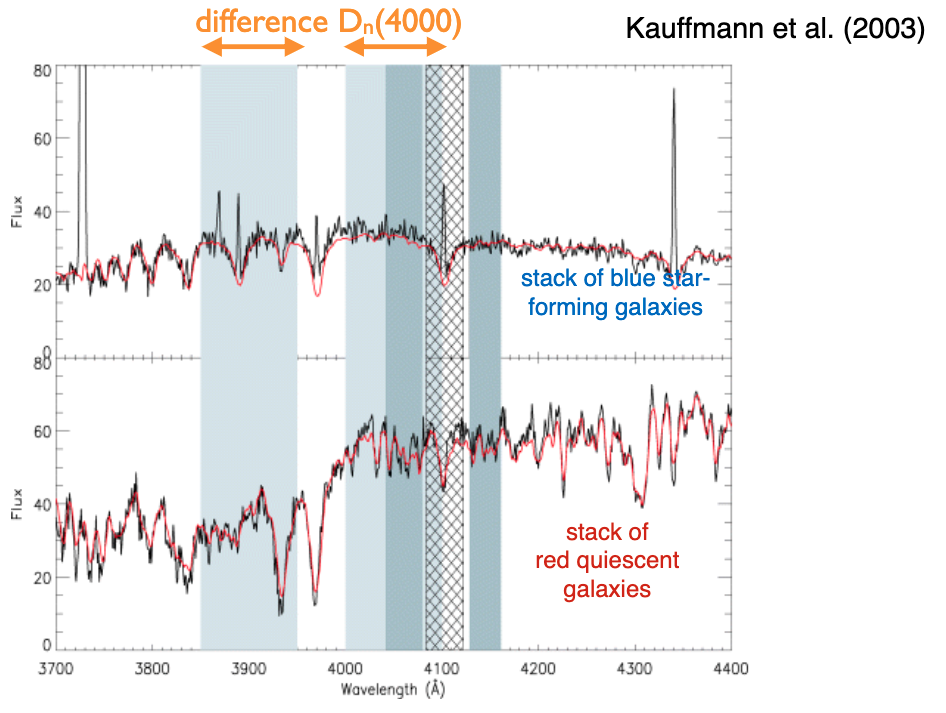
\includegraphics[width=0.66\textwidth]{figs/Screen Shot 2021-09-02 at 9.42.59 AM.png}
    \caption{Star forming galaxies have a very small break, but the red galaxies have a very large break near $4000\AA$. }
    \label{fig:my_label}
\end{figure}

Here is the 4000 Angstrom break as a function of both age and metallicity:

\begin{figure}
    \centering
    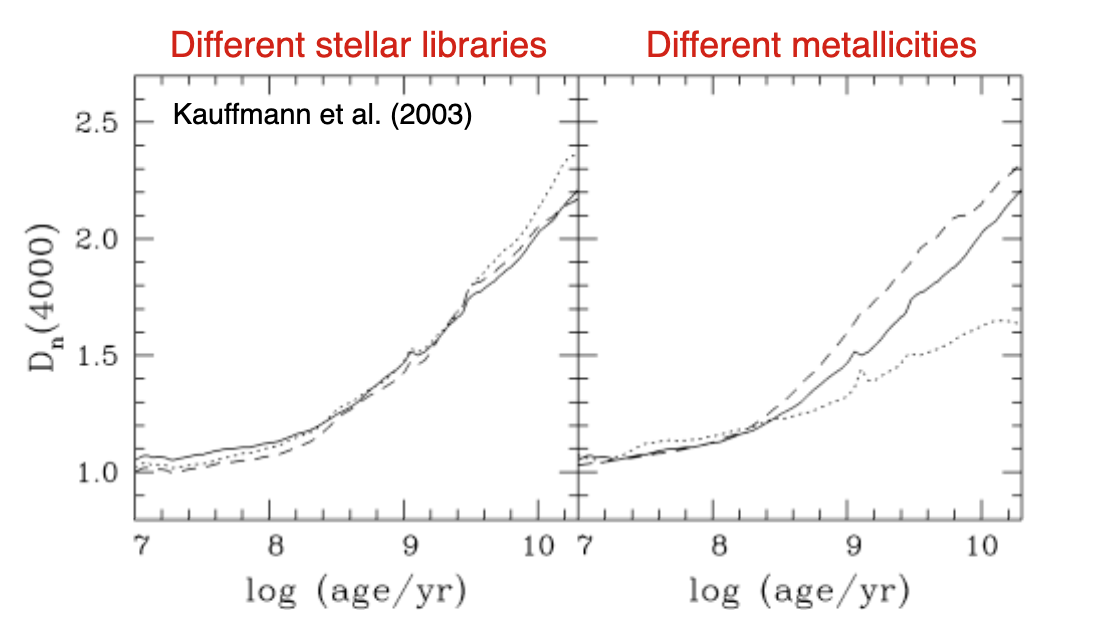
\includegraphics[width=0.66\textwidth]{figs/Screen Shot 2021-09-02 at 9.43.15 AM.png}
    \caption{The 4000 Angstrom break. }
    \label{fig:4000angbreak}
\end{figure}

So, the takeaway is that the $4000\AA$ break is a much better measurement of age compared to broadband photometry, but much more expensive. There's also a pretty strong signal to noise requirements needed for D4000 measurements. 

D4000 measurements are tough with k-corrections in the mix as well since we need to know the intrinsic shape of the spectrum, which is much harder for high redshift galaxies. 

\subsection{Stellar metallicity - mass relation (Gallazzi et al., 2005)}

At higher masses, stars are more metal-rich. As you go to lower masses, we have lower metallicity. Under the hood, star formation is generating metals. Massive galaxies have more star formation, and thus more metals, to zeroth order.

\begin{figure}
    \centering
    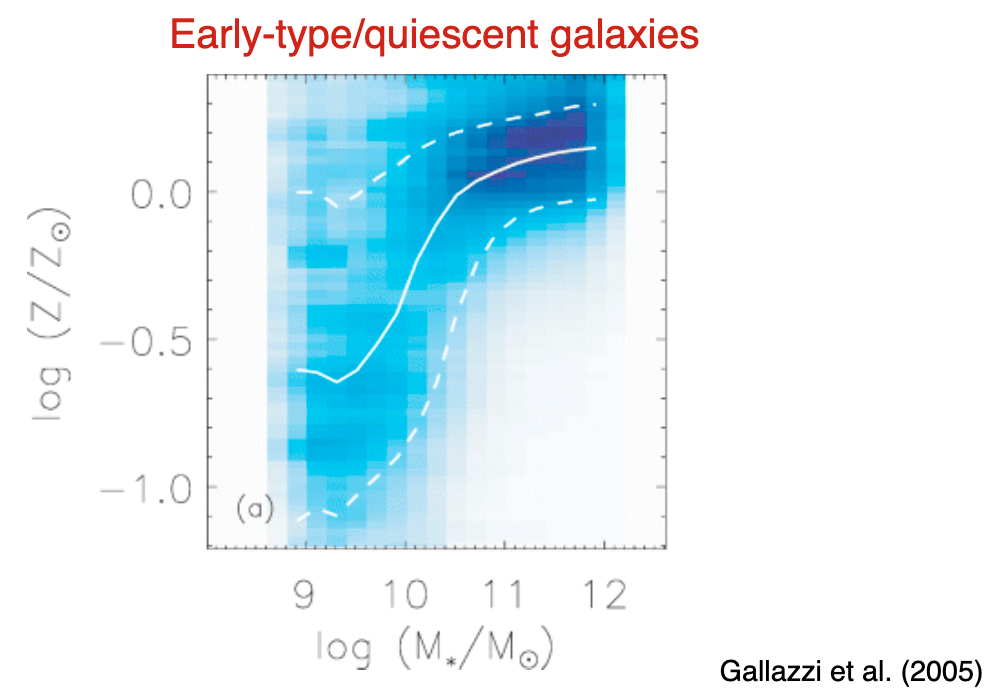
\includegraphics[width=0.66\textwidth]{figs/Screen Shot 2021-09-02 at 9.43.55 AM.png}
    \caption{Stellar metallicity-mass relation for early-type galaxies.}
    \label{fig:z_m_relation}
\end{figure}

For \textbf{late type galaxies}, this is more complicated but gives a similar trend. 

\begin{figure}
    \centering
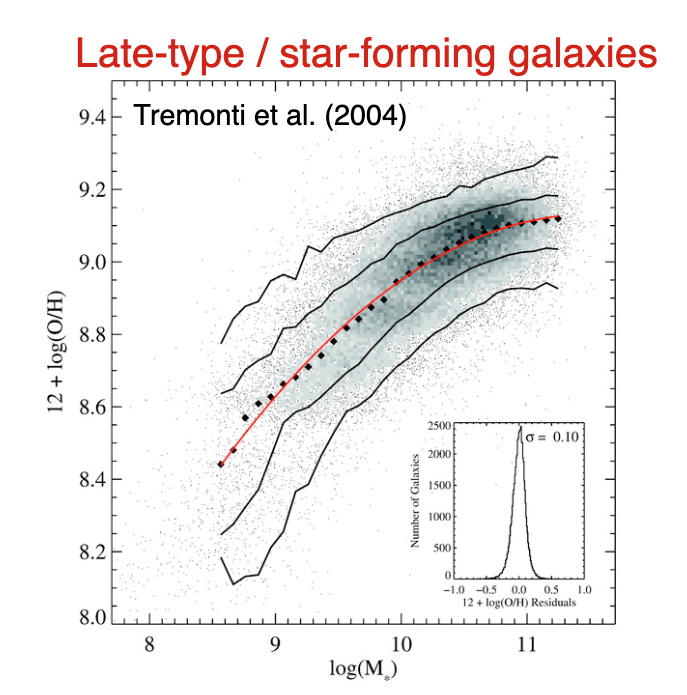
\includegraphics[width=0.66\textwidth]{figs/Screen Shot 2021-09-02 at 9.44.18 AM.png}
    \caption{Stellar metallicity-mass relation for late-type galaxies.}
    \label{fig:z_m_relation_late}
\end{figure}

How do you make a measurement like this? Ionized HII regions emit oxygen lines in late-type galaxies. This doesn't happen in early type galaxies! 

We will continue next time with the late-type slope in the color-mass plot! 

\section{September 3, 2021: Global properties, galaxy correlations, and statistics}

\subsection{Measuring gas-phase metallicity}

What is going on with the fiber versus total spectra in the SDSS data? SDSS is a fiber fed system, with each fiber being really tiny. As a result, only the central regions are getting spectra! 

We are thus assuming that in the central region, oxygen emission comes only from star formation. It turns out that AGN also create emission line patterns which complicate things! 

In our problem set, we are asked for gas-phase metallicity for our galaxies, so what do we do? For our homework, use total fluxes and not fiber fluxes! 
\subsection{Brief Review of Last Time: Color Sequences, }

Remember the $u-r$ color slope is primarily drive by the metallicity (mass-metallicity relation) for early type galaxies. 

Late-type galaxies are driven by star-formation properties. The way we can see this most clearly is the star formation rate-stellar mass relation (Samir et al, 2007):

\begin{figure}
    \centering
    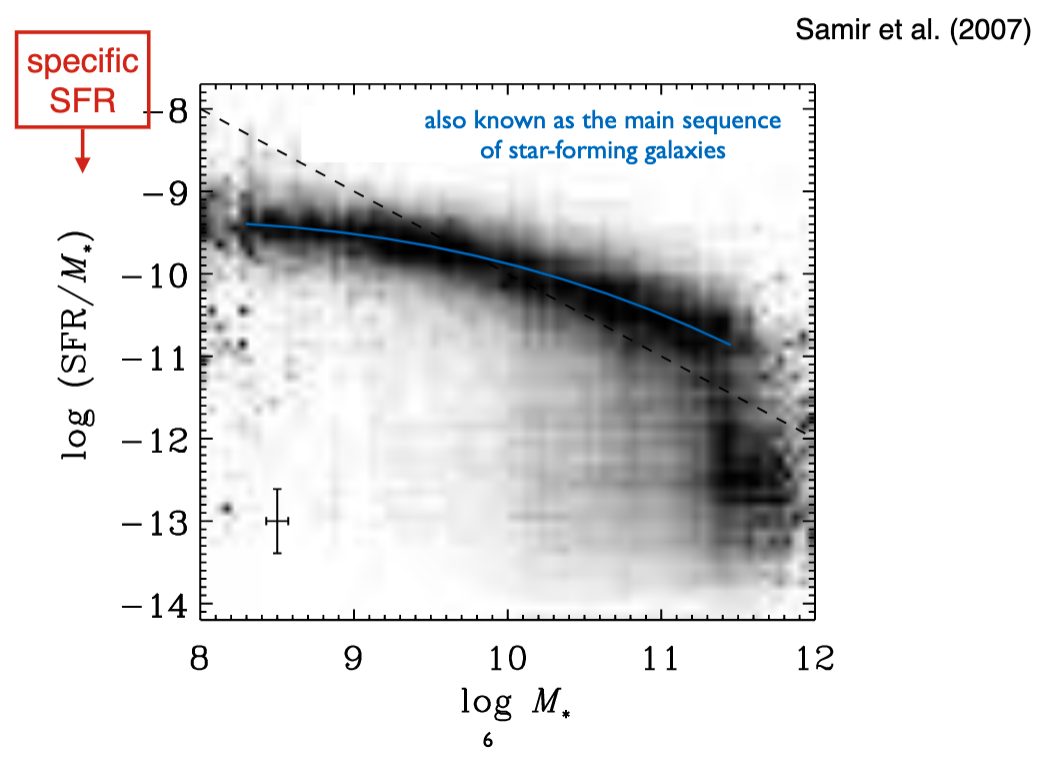
\includegraphics[width=0.75\textwidth]{figs/Screen Shot 2021-09-03 at 11.28.46 AM.png}
    \caption{sSFR-stellar mass relation. }
    \label{fig:ssfr_sm}
\end{figure}

This isn't the most obvious thing to plot, however. It'd be more obvious to plot star formation rate versus the stellar mass (star-forming main sequence). The shape changes when we plot the specific star formation rate. So what does this tell us/what is the interpretation?

As we go to higher masses, the \textbf{star formation rate per unit mass is lower because it's less efficient}. One way to think about this (since the previous statement is pretty empty): low mass galaxies have younger populations which have formed more recently (and thus have no converted mass into stars yet because the potential is shallower). Another explanation is that larger galaxies have had time to spread mass out over the whole halo (where gas density is too low to form stars). 

\subsection{Stellar mass-halo mass relation}

\begin{figure}
    \centering
    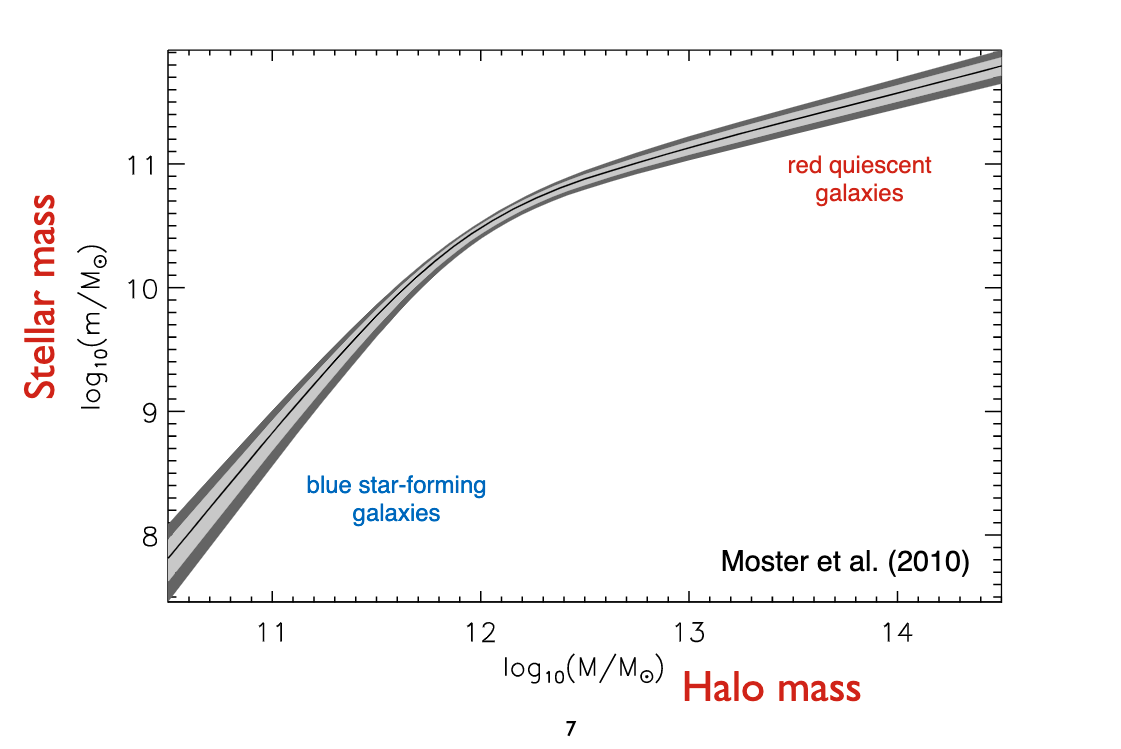
\includegraphics[width=0.75\textwidth]{figs/Screen Shot 2021-09-03 at 11.29.07 AM.png}
    \caption{Stellar mass-halo mass relation (Moster 2010). }
    \label{fig:smhm_relation}
\end{figure}

One of the ideas in galaxy formation is that the dark matter halo drives galaxy formation moreso than anything else. The halo mass should thus determine the evolution of the galaxy as a whole. It sets the potential, temperatures of gas (kinematic temperature), accretion rate (mass inflow rate), etc. \textbf{The problem is that measuring halo masses is really difficult!}

We can assign galaxies to halos with \textbf{abundance matching}, shown in Figure~\ref{fig:smhm_relation}, giving rise to the stellar-mass halo-mass relation (SMHM, SMH relation). The most massive stellar and dark galaxies are red, quiescient galaxies. At the low end, there are blue star-forming galaxies. 

This leads to one of the most important plots in the course:

\begin{figure}
    \centering
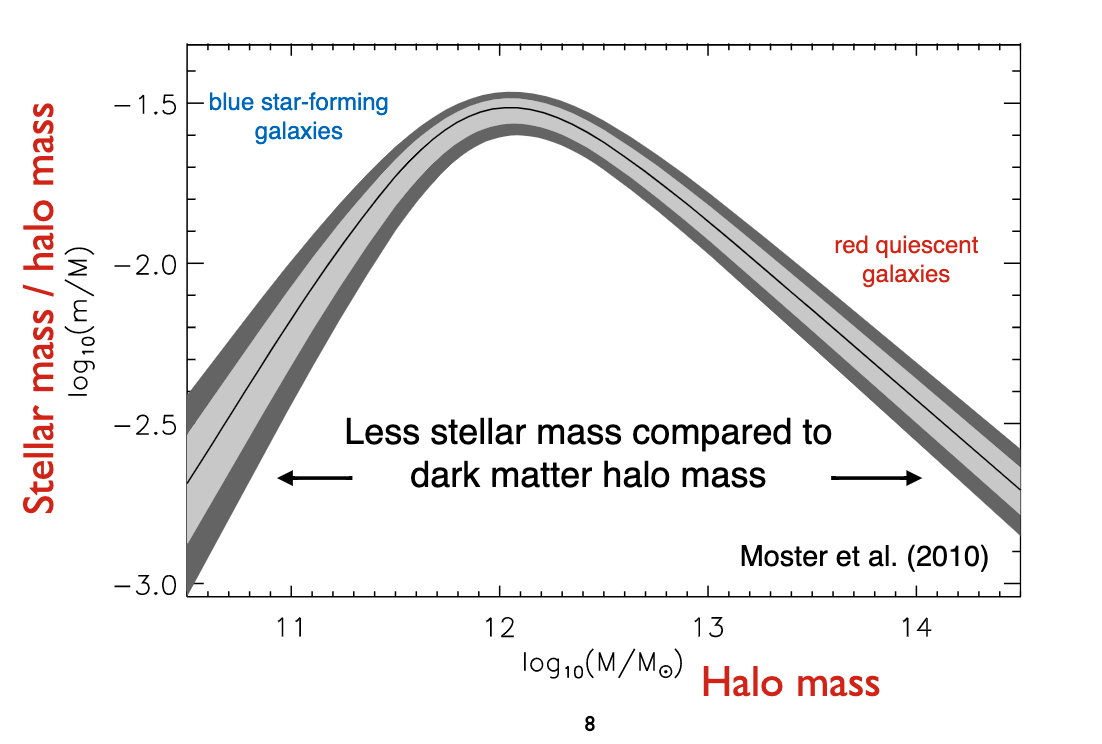
\includegraphics[width=0.75\textwidth]{figs/Screen Shot 2021-09-03 at 11.29.23 AM.png}
    \caption{Stellar mass-halo mass ratio vs. halo mass. This is saying that, as you go to really low or high mass haloes, there is less stellar mass! \textbf{Per unit halo mass, really massive and really low-mass galaxies are inefficient at star formation.} The peak is where star formation in the most efficient!}
    \label{fig:smhm_ratio}
\end{figure}


\subsection{Galaxy Sizes}
\subsubsection{Sersic (1968) Profiles}

The generalized version is:

\begin{equation}
    I(R) = I_0 e^{-\beta_n\left(R/R_e\right)^{1/n}} = I_e e^{-\beta_n\left(\left (R/R_e\right)^{1/n}-1\right)}
\end{equation}

Here, $I_0$ is the central intensity, $\beta_n$ is a scale factor, $n$ is the Sersic index, $R_e = R_{1/2}$ is the effective radius or the half-light radius. 

You often see this written in terms of surface brightness, which is just the magnitude form. 

There are \textbf{two specific cases of the Sersic profile}. For \textbf{early type galaxies}, we have \textbf{deVaucouleur's Law}:

\begin{equation}
    I(R) = I_e e^{-7.7\left[\left(R/R_e\right)^{1/4} - 1\right]}
\end{equation}

This is a Sersic with $n = 4$ and $\beta_n = -7.7$. If we plot $\mu$ versus $r^{1/4}$, this is a straight line:

% \begin{figure}
%     \centering
%     \includegraphics{figs/}
%     \caption{Mu versus r making a straight line. }
%     \label{fig:mu_r}
% \end{figure}

Late-type galaxies are even more difficult to fit. For late-type galaxies, we have:

\begin{equation}
    I(r) = I_0 e^{-r/h}
\end{equation}

where $I_0$ is the central surface brightness, $h$ is the scale length ($1e$ folding of light). In this case, plotting $\mu$ versus $r$ alone gives the straight line. 

\subsection{Stellar mass-size relation (Shen et al., 2003)}

\begin{figure}
    \centering
    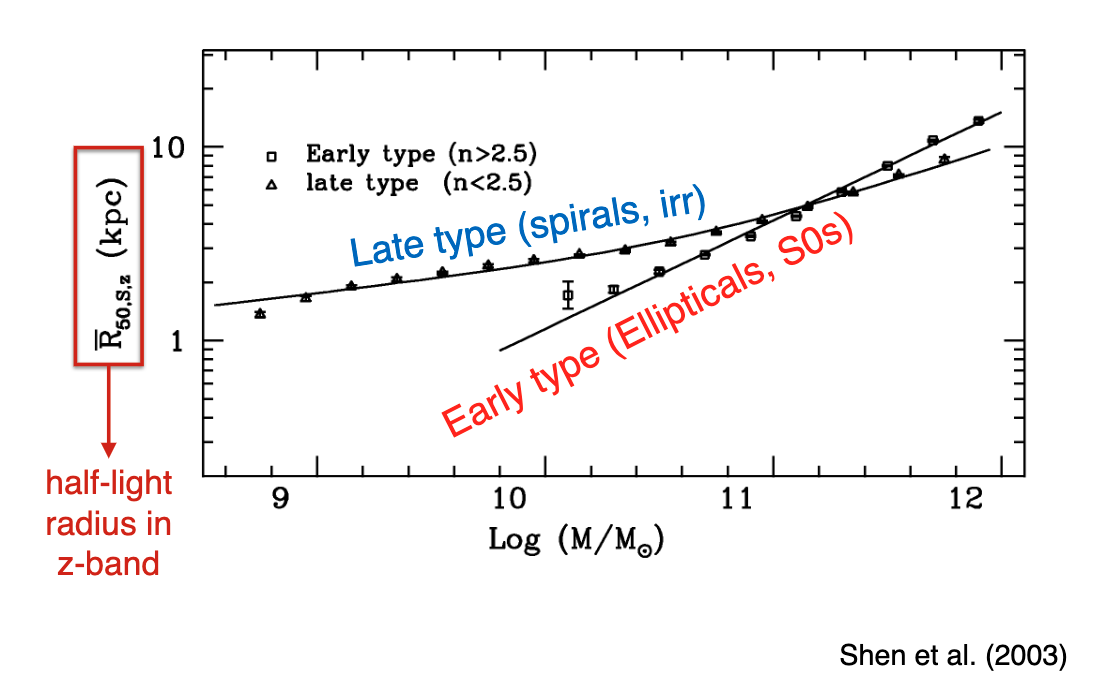
\includegraphics[width=0.75\textwidth]{figs/Screen Shot 2021-09-03 at 11.29.54 AM.png}
    \caption{Stellar mass-size relation. }
    \label{fig:smsr}
\end{figure}

\subsection{Measuring galaxy sizes and Sersic indices}

Large sersic indices are peaky toward the middle (ETGs), smaller values (late-type) are toward the outskirts. 

\subsection{Galaxy sizes over cosmic time}

Good to know that sizes are not constant over time, and we will come back to this. 

\subsection{Relation with Environment}

\begin{figure}
    \centering
    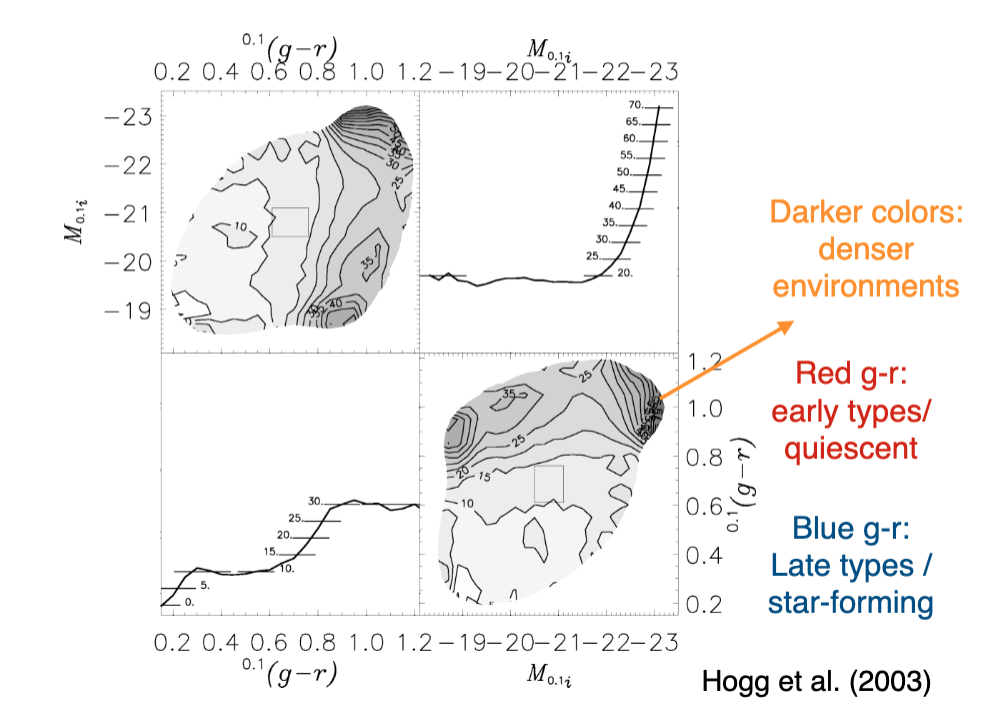
\includegraphics[width=0.75\textwidth]{figs/Screen Shot 2021-09-03 at 11.30.25 AM.png}
    \caption{Rleation with environment. Bottom right: Contours are density, with darker colors being denser environments (number per volume). In higher density environments, you find early type galaxies. }
    \label{fig:env}
\end{figure}

\begin{figure}
    \centering
    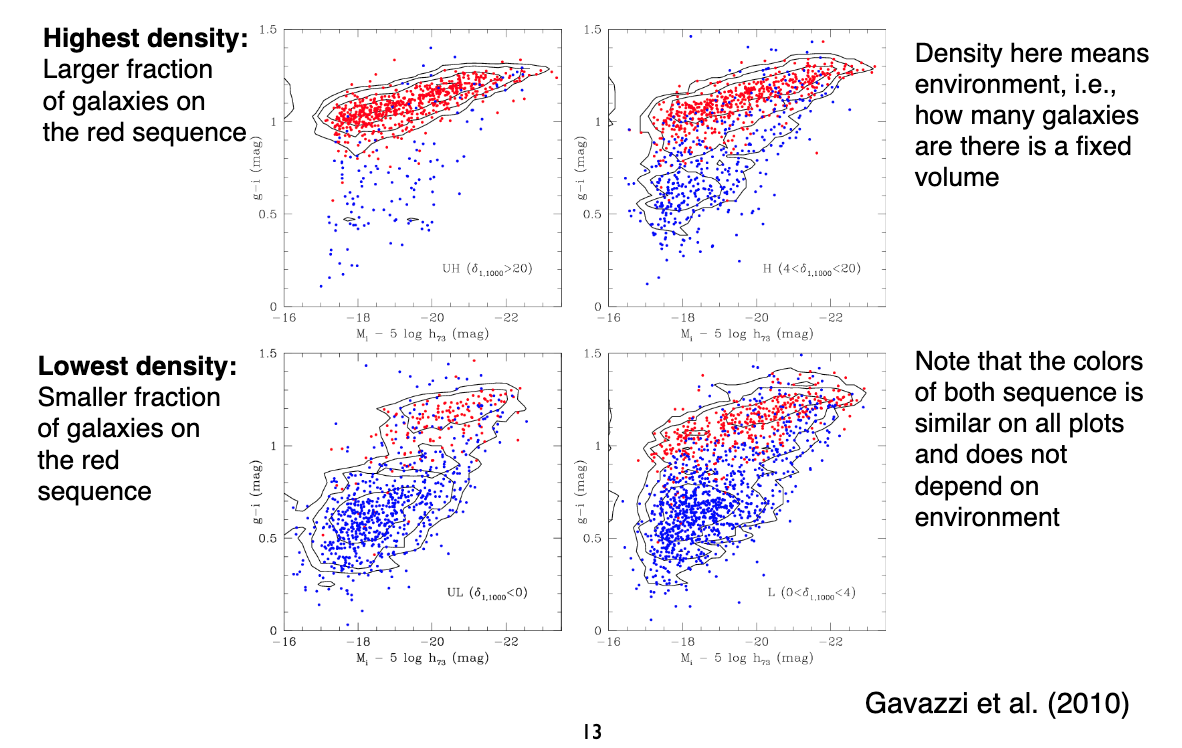
\includegraphics[width=0.75\textwidth]{figs/Screen Shot 2021-09-03 at 11.30.48 AM.png}
    \caption{Color-magnitude diagrams in different environments (Gavazzi et al. (2010).  }
    \label{fig:cmd_env}
\end{figure}

\subsection{Disentangling environment, mass, morphological type, and Sersic parameter (van der Wel 2008. }

Left hand column x-axis is number per volume. 

\subsection{Staistical properties of the galaxy population}

Look at the M87 field. We can start to plot the number of galaxies as a function of luminosity bin since they are all at the same (rough) distance. Our theories can make predictions on this!

\subsection{The luminosity function of galaxies}

First posited by Schechter (1975), we have the Schechter luminosity function. For better or worse, there are no physical bases for this even though it works really well!

\begin{equation}
    \Phi(L) \,\mathrm{d}L = \Phi_* \left(\frac{L}{L_*}\right)^{\alpha} e^{-L/L_*} \, \mathrm{d}\left(\frac{L}{L_*}\right)
\end{equation}

$L_*$ is the inflection point in the luminosity function, $\alpha$ is the ``faint-end slope'', $\Phi_*$ is a normalization. Note that the units of $\Phi$ are number/volume. Sometimes this is further divided into magnitude bins. 

When $L \ll L_*$, we have power law behavior with $\alpha$ dominating. For $L \gg L_*$, we have exponential decline dominating. In the local universe, the Milky Way is approximately an $L_*$ galaxy. In physical units, we have:

\begin{equation}
    L_\text{B-band}^\text{MW} \sim 10^{10} L_\odot
\end{equation}

\subsection{Peculiar Motions}

To get a luminosity, we first need a distance! Occasionally, you see a \textbf{huge} scatter in the relationship because of peculiar velocities of things like the Virgo cluster. 

This introduces the concept of \textbf{Malmquist bias}. You can see brighter objects farther away:

\begin{figure}
    \centering
    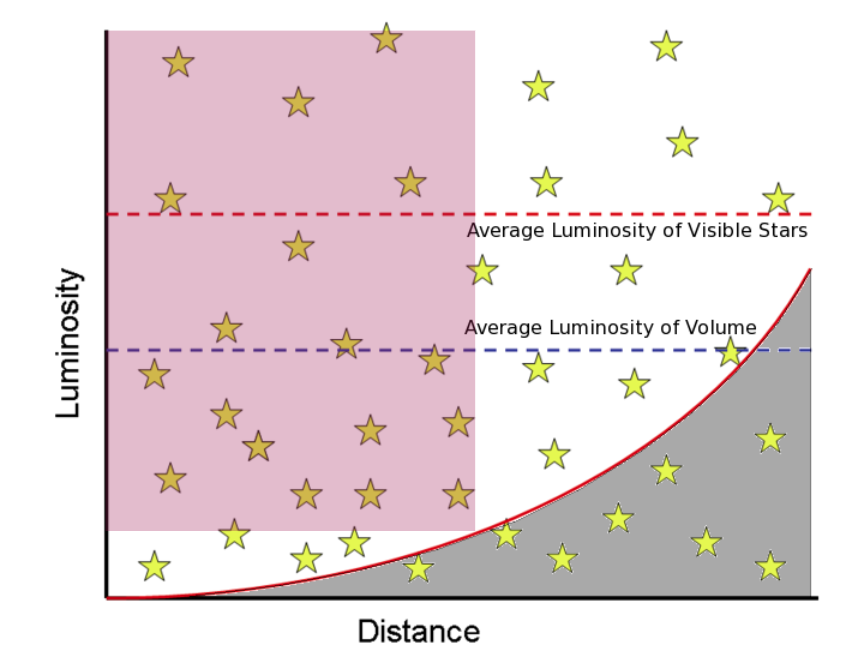
\includegraphics[width=0.75\textwidth]{figs/Screen Shot 2021-09-03 at 11.31.27 AM.png}
    \caption{Malmquist bias. }
    \label{fig:malm}
\end{figure}

Perhaps most obvious fix is a luminosity cutoff, but this has disadvantages in that you impose a distance cutoff and also you're throwing out data. The better solution is a $1/V_{max}$ correction:

\begin{figure}
    \centering
    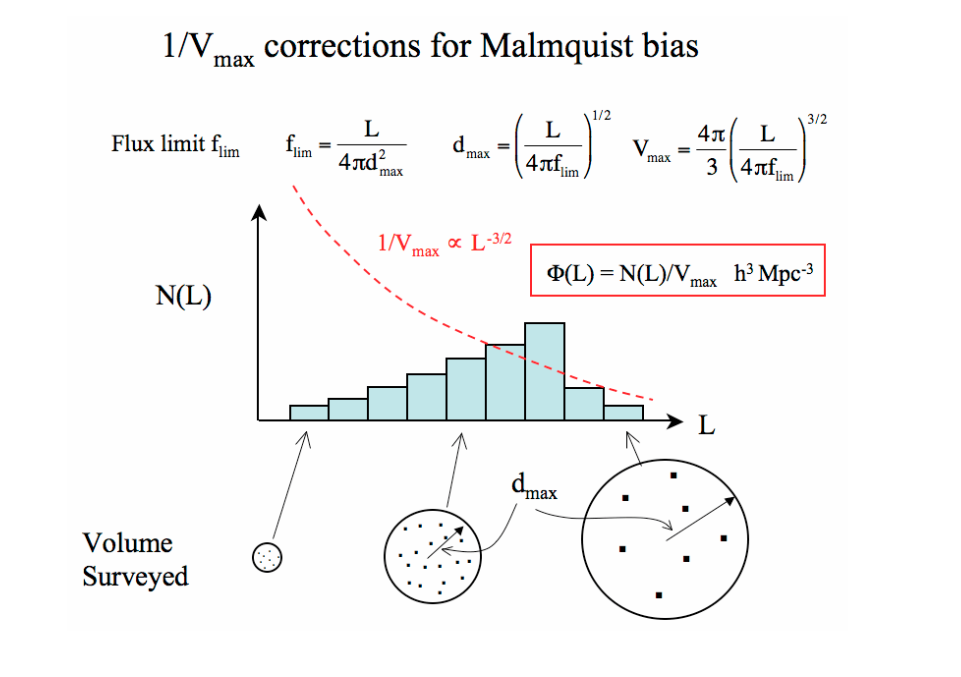
\includegraphics[width=0.75\textwidth]{figs/Screen Shot 2021-09-03 at 11.31.42 AM.png}
    \caption{Malmquist bias solution as a $1/V_{max}$ correction. }
    \label{fig:malm_fix}
\end{figure}

\section{September 8, 2021: Finish galaxy statistics; stellar populations; stellar evolution review}

\subsection{Luminosity Function for Different Hubble Types}

Why does the Schechter function work? See Binggeli (1998). The composite of individual galaxy functions form a Schechter function, but each individual function does not! Is this accurate? Maybe not...are these complete at the faint end? To first order, yes. Bot nothing is first order.

\subsubsection{Challenges}

\begin{itemize}
    \item Need to know distances; redshifts for low-z galaxies reflect distance and peculiar motion
    \item Low surface brightness galaxies are hard to detect.
    \item Malquist bias: brighter galaxies can be traced to larger distances than fainter galaxies. We can correct by only considering range of luminosity and distance; or you can apply volume corrections for each luminosity. 
\end{itemize}

\subsubsection{Vmax Correction, Revisited}

\subsection{Luminosity Functions as a function of color (Blanton 2001)}

Red galaxies dominate the bright end of the luminosity function -- the biggest are the brightest! The blue galaxies dominate the faint end. This is not totally a surprise! Remember the stellar mass versus color diagram! 

\subsection{Luminosity Function as a function of environment (Christlein 2000)}

There are more galaxies in denser environments. Also, the faint end slope gets steeper in low density environments. There are man more low mass galaxies in dense environments. 

\subsection{Luminosity and Mass Functions (Yang et al. 2009)}

Redder galaxies have higher mass-to-light ratios $\Upsilon$, and thus the red function moves to the right compared to the blue function when going from luminosity to mass. Working in mass function space \textbf{is much better} than in luminosity space, but you need way more data to get masses. 

\subsection{Physical Origin of the Luminosity Function}

Ratio of these two lines give us the plot from last time of the halo mass versus stellar mass per halo mass plot (with peak efficiency near the MW). 

\subsection{Evolution of the Mass Function (with redshift) [Muzzin et al 2013]}

The normalization shifts, for sure, but you also start to see other patterns emerge. At high redshift ($z\sim2$), the functions are more or less on top of each other. We can see changes in galaxy populations!

\textbf{The mass function can be used to trace the build up of stellar mass in both star-forming and quiescent galaxies over cosmic time.}

\subsection{Evolution of the UV Luminosity Function (Bouwens et al 2000)}

UV Luminosity functions (UVLF) can be used to trace the evolution of the SFR density over cosmic time. At high redshift, we have low number densities of galaxies because galaxies have not formed yet! We can also look at the confidence intervals for the Schecter fit parameters, and we see the evolution!


\subsection{Star formation history of the Universe}

Inferred by integrating the UV luminosity function. This is basically the star formation rate per unit volume as a function of redshift. Going back in time, cosmic SFR peakrs around $z\sim2-3$, and declines steeply to high redshift. The peak epoch was around $2-3$ billion years after the Big Bang.

To make these measurements, we get a UVLF at a redshift, fit a Schechter function, integrate to some limit (giving total UV luminosity at that redshift), use a stellar population model which gives a number of stars and masses, and then get star formation rate. 

The blue line above is the integrated UV luminosity. The red shows what happens when we dust correct. No dust was really present at a redshift of $z>6$. Dustiest galaxies are near $z\sim 2-3$. Early galaxies were low metallicity and thus couldn't enrich with dust until SFR kicked in (with other chemical evolution). 

\subsection{Quiz!}

\begin{itemize}
    \item The specific star formation rate is slightly lower though for more massive star-forming galaxies on the star forming main sequence, and thus these galaxies are slightly more evolved and redder. Also think about the color-mass relation -- smaller mass has lower $u-r$ and thus is bluer. 
\end{itemize}

\section{September 10, 2021: Stellar Evolution and Stellar Populations}

\subsection{Background}

\begin{itemize}
    \item Stellar spectra and spectral types
    \item Stellar evolution
    \item Stellar initial mass function
    \item Dust attenuation and emission
    \item Star formation histories
    \item Stellar population synthesis modeling
\end{itemize}

\subsection{A quick thing about Problem 3e: Photon and Energy Counting Detectors}

Here's the issue. We wrote down an equation:

\begin{equation}
    \int_0^\infty S_\lambda F_\lambda \mathrm{d}\lambda
\end{equation}

This equation is ambiguous. It's not specific enough. This $F_\lambda$ and $S_\lambda$ have different units, actually. There are actually units attached to $S_\lambda$ that are ignored, typically. The units don't make sense because $S_\lambda$ is kind of like a ``fraction of photons,'' and thus we have to convert to number of photons instead of the energy of photons. 

Apparently, here is the solution -- don't derive from first principles, but think dimensionally. Take $F_\lambda$ and go from energy to number. We do this by:

\begin{equation}
    F_\lambda \rightarrow \frac{F_\lambda}{E} = \frac{\lambda F_\lambda}{hc}
\end{equation}

This is a \textbf{photon counting detector}, not an \textbf{energy counting detector}. In that case, it's more complicated, and we have $\lambda^2 F_\lambda S_\lambda \mathrm{d}\lambda$.

\subsection{Stellar Evolution}

\subsubsection{HR Diagrams: Main Sequence}

\begin{figure}
    \centering
    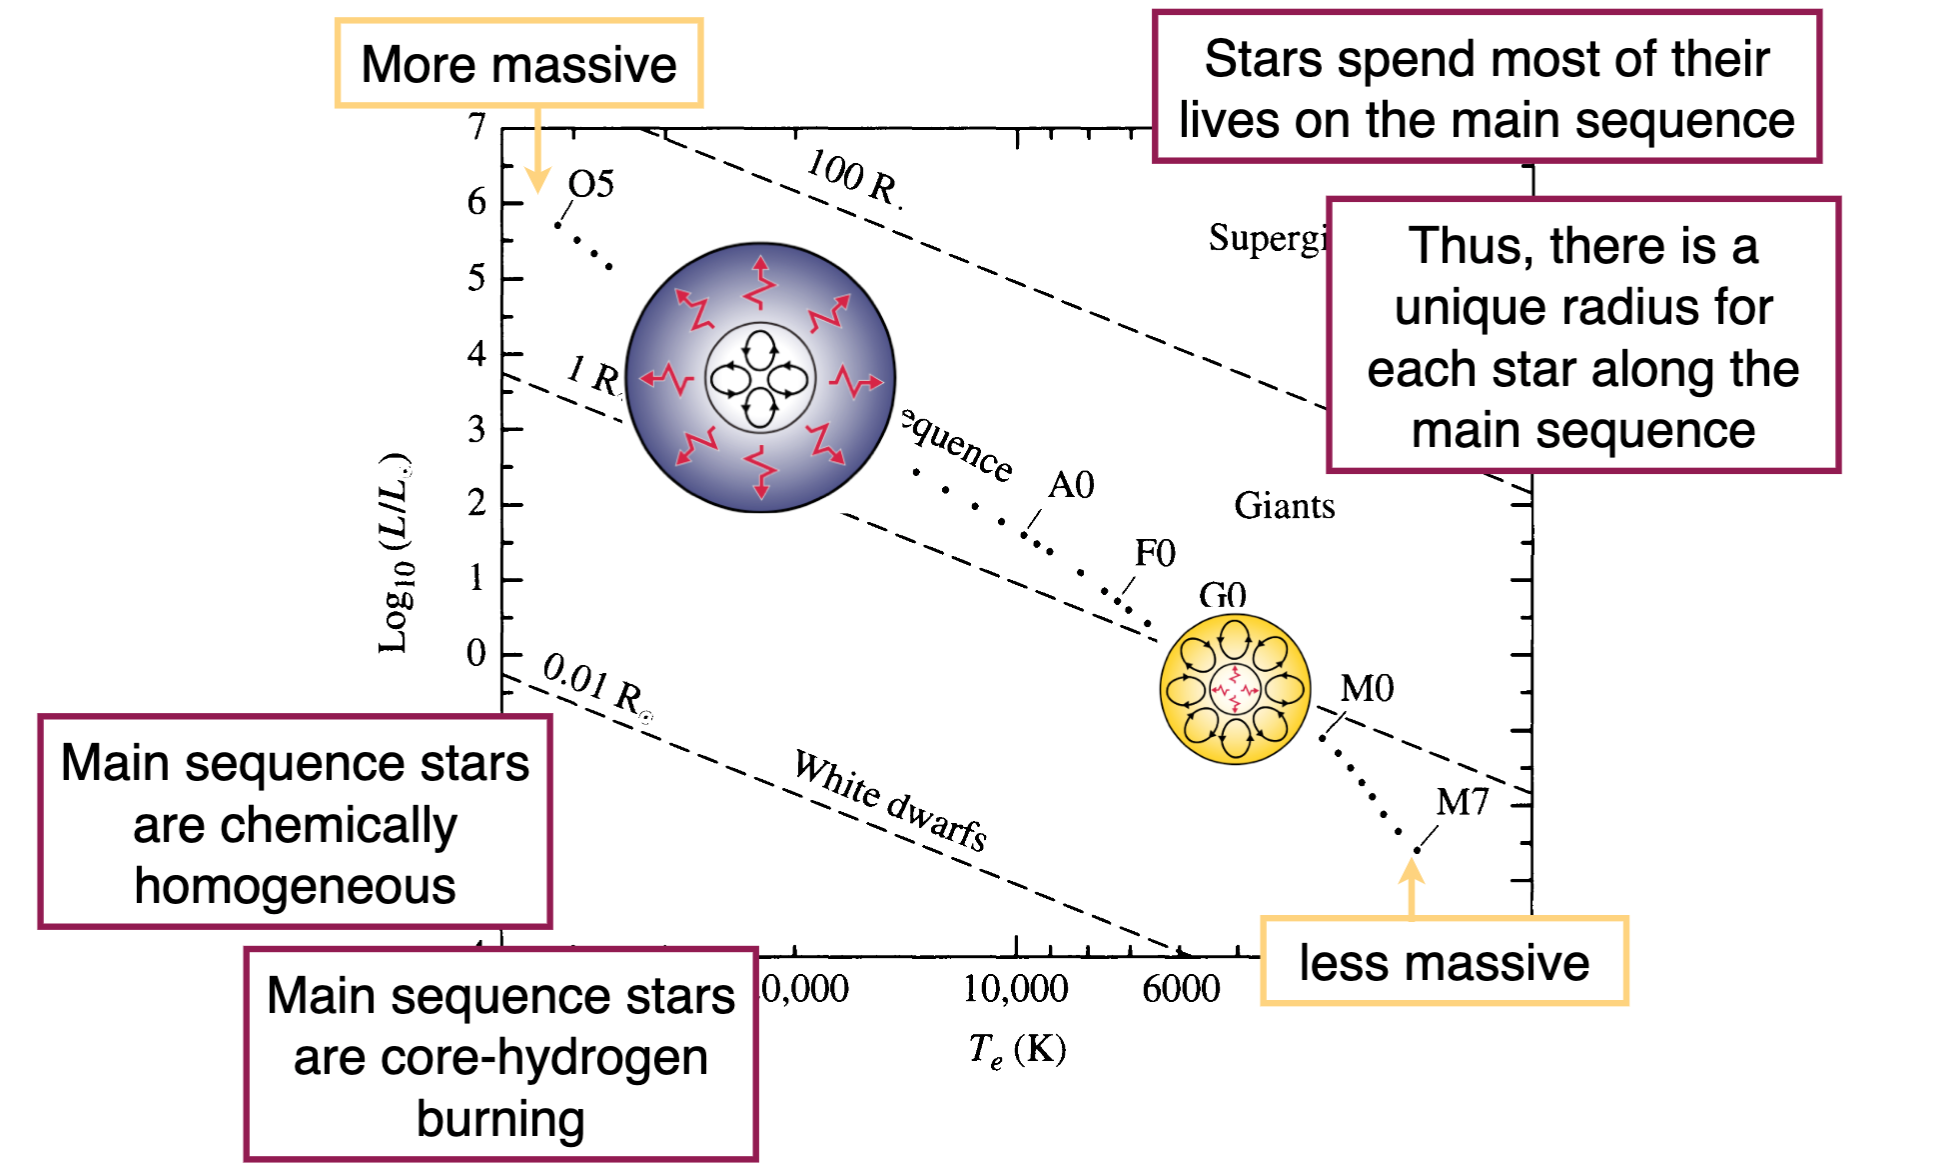
\includegraphics[width=0.66\textwidth]{figs/Screen Shot 2021-09-15 at 9.04.35 AM.png}
    \caption{HR Diagram.}
    \label{fig:HR}
\end{figure}

\begin{itemize}
    \item Stars spend most of their life on the main sequence, defined as core hydrogen burning. 
    \item Thus, there is a unique radius for each star along the main sequence. We infer a radius with the Stefan-Boltzmann law (derived from blackbodies, good for stars). We measure a luminosity $L = 4\pi Fd^2$ and temperature from spectra or colors:
    \begin{equation}
        L = 4\pi R^2 \sigma T^4
    \end{equation}
    \item More massive stars in the top left; less massive in the bottom right. 
    \item Main sequence stars are chemically homogeneous
    \begin{itemize}
        \item Main sequence stars are in hydrostatic equilibrium.
    \end{itemize}
    \item Low mass stars and high mass stars differ in energy transport. Low mass has convection exterior; high mass stars have convection in the core. Determined by adiabatic temperature gradients. If the temperature gradient is super adiabatic, you have convection. 
\end{itemize}

\subsubsection{Difference in Chemical Composition}
\begin{figure}
    \centering
    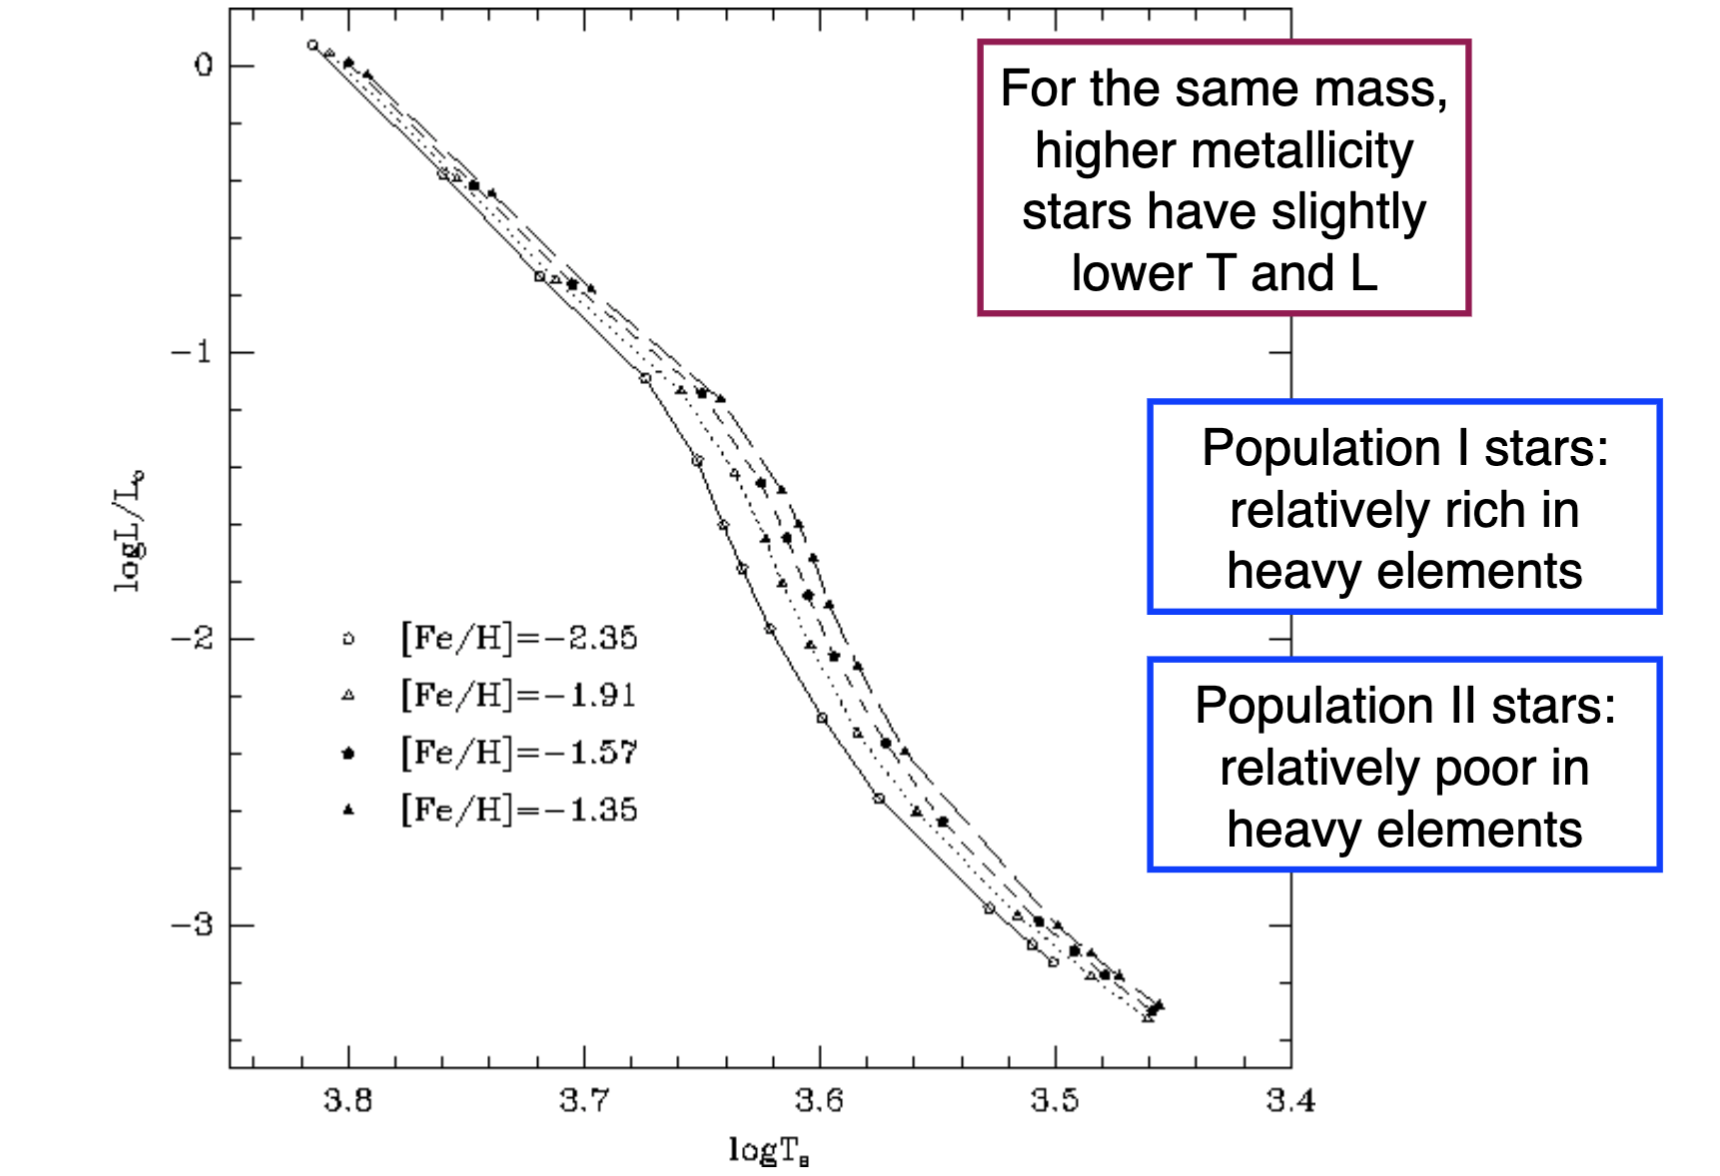
\includegraphics[width=0.66\textwidth]{figs/Screen Shot 2021-09-15 at 9.04.48 AM.png}
    \caption{Differences in chemical composition.}
    \label{fig:zcomp}
\end{figure}

\begin{itemize}
    \item [Fe/H] is the amount of iron-content of a star relative to the sun. The more negative, the more metal poor. 
    \item For the same mass, high metallicity is cooler and less luminous. 
    \begin{itemize}
        \item Pop I: Relatively rich in heavy elements
        \item Pop II: Relative poor in heavy elements
        \item Pop III: Metal free stars. 
    \end{itemize}
\end{itemize}

\subsubsection{Relation between luminosity and mass}

Over the entire main sequence, it's almost $L\sim M^{3.5}$. 

\begin{figure}
    \centering
    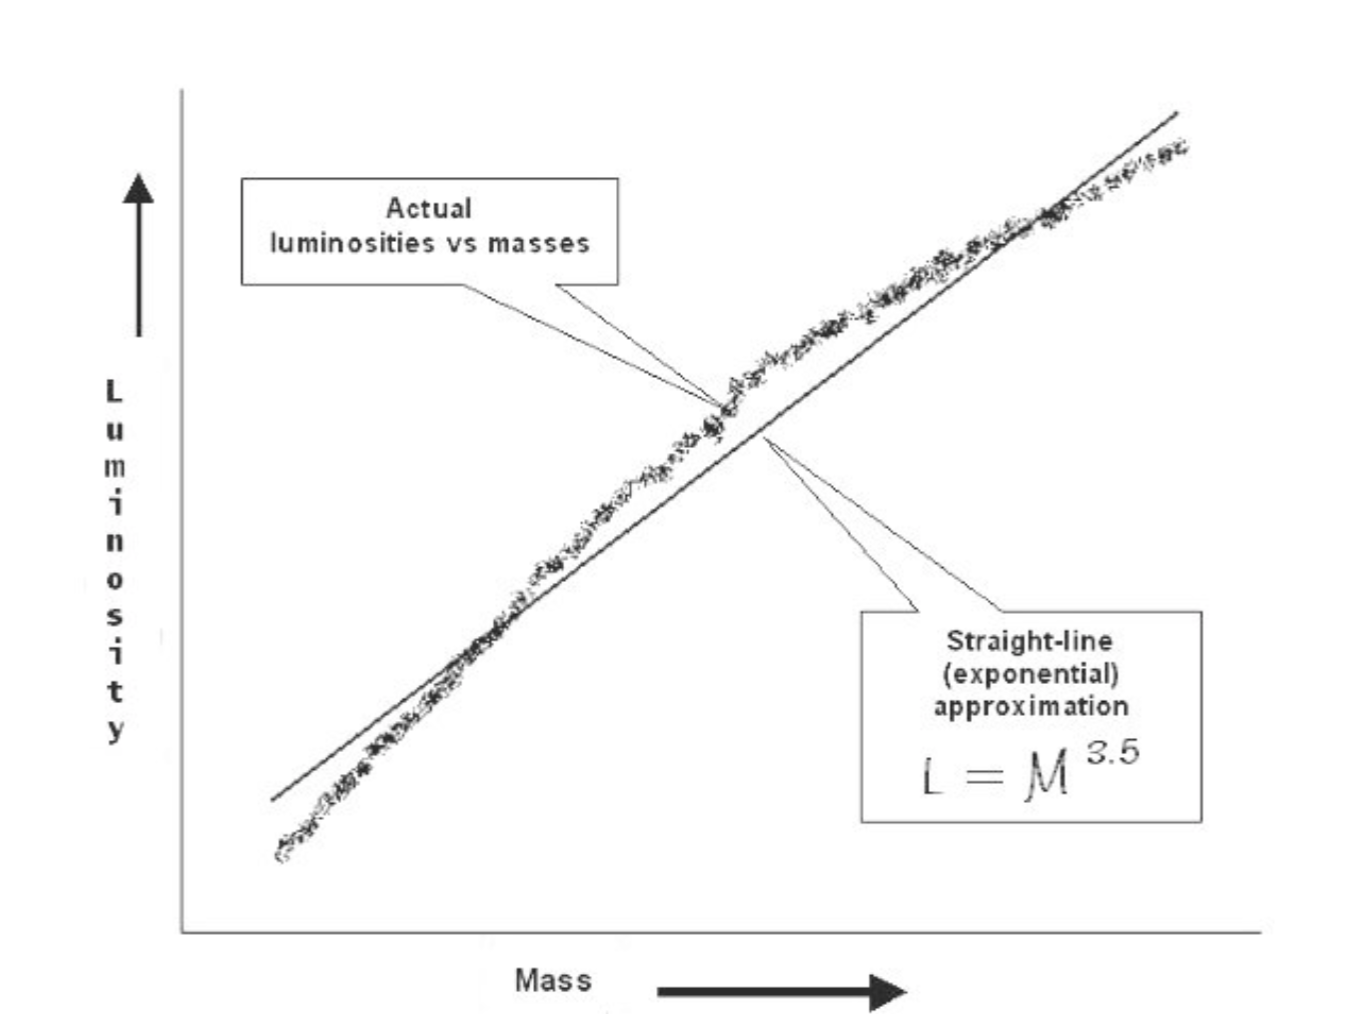
\includegraphics[width=0.66\textwidth]{figs/Screen Shot 2021-09-15 at 9.04.57 AM.png}
    \caption{Proportionality. }
    \label{fig:prop_approx}
\end{figure}

\subsubsection{Post MS Evolution}

Stars spend about $90\%$ of their time on the MS. After the core is exhausted of hydrogen, we enter the \textbf{sub-giant branch}. The core contracts and heats. Hydrogen burning shell gets formed around the Helium core. Energy release from H-envelope leads to expansion of intermediate layers, and thus a drop in temperature $T$. 

\begin{figure}
    \centering
    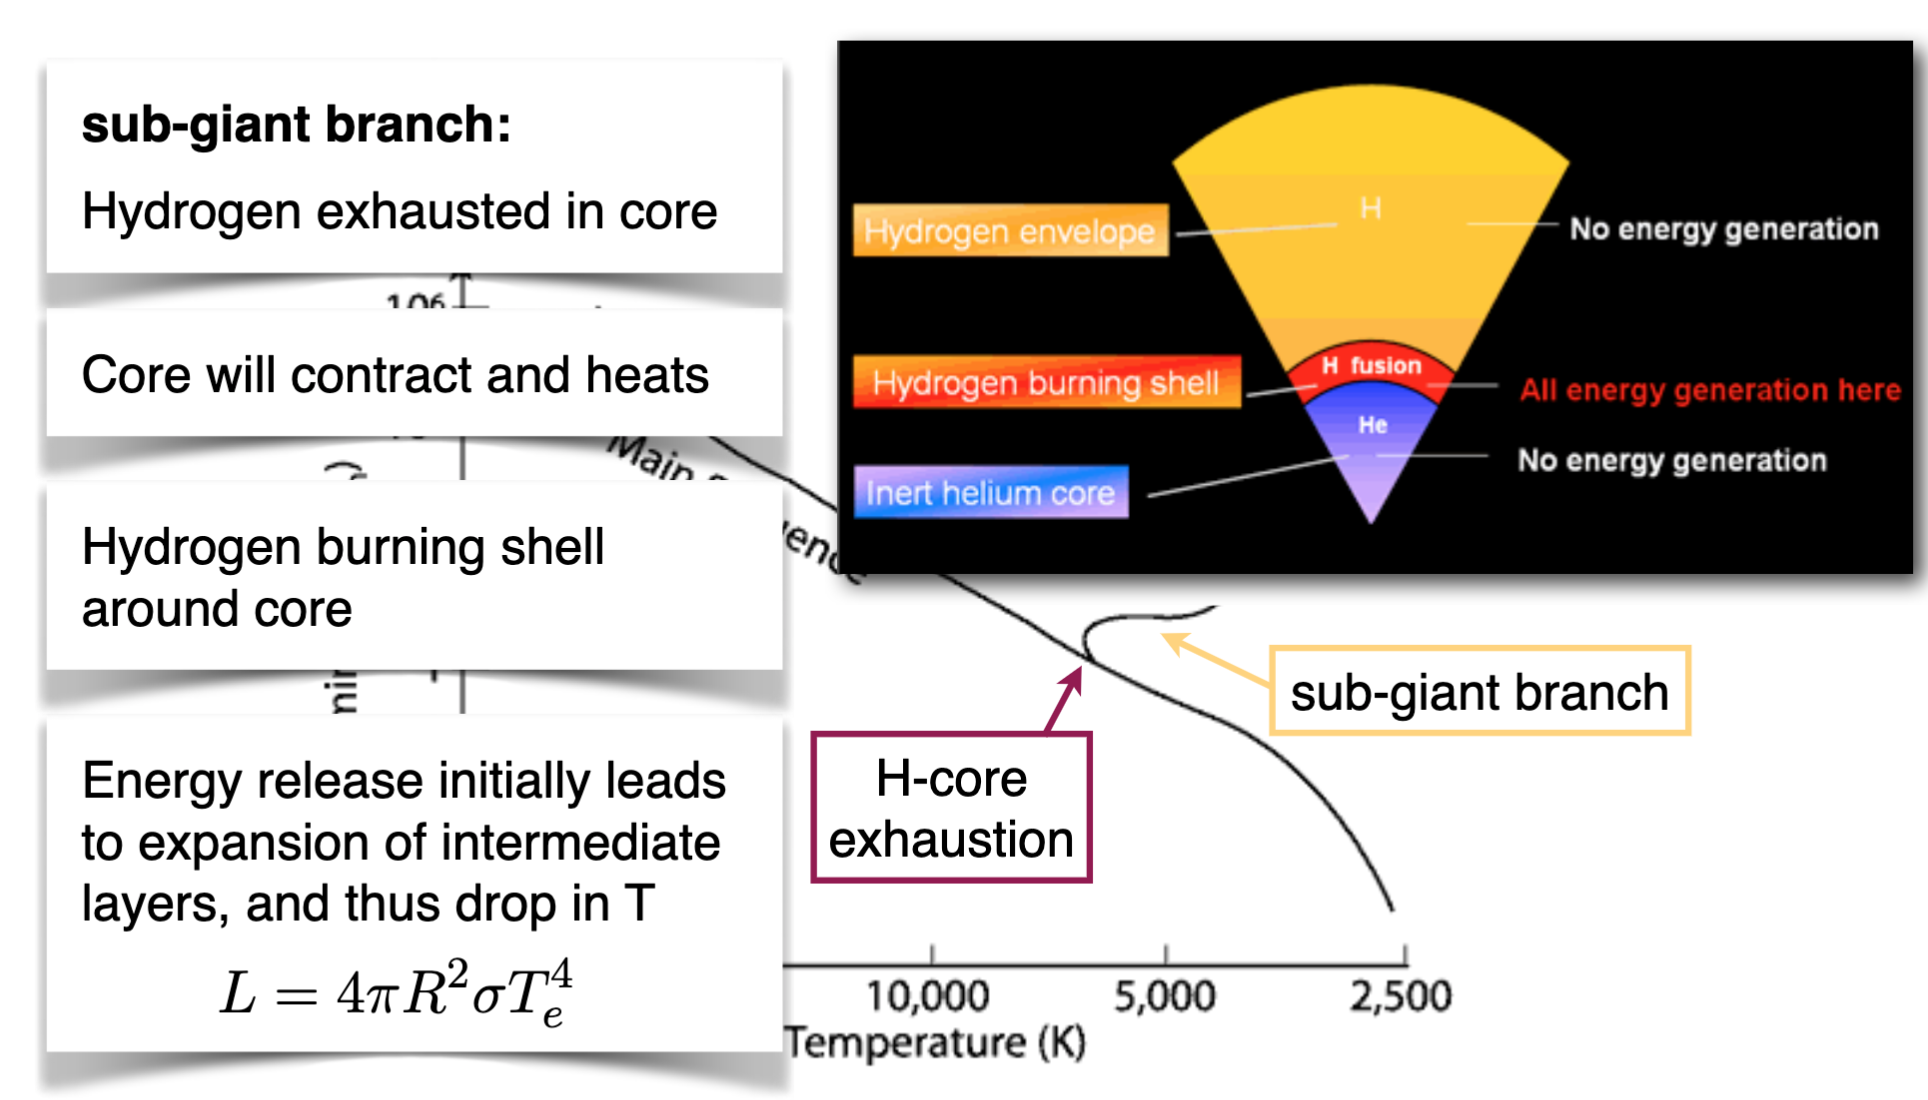
\includegraphics[width=0.66\textwidth]{figs/Screen Shot 2021-09-15 at 9.06.26 AM.png}
    \caption{Sub-giant branch.}
    \label{fig:subgiant}
\end{figure}

Then, we have vertical evolution on the HR diagram called the \textbf{red giant branch}. There is an ascent phase during which the core is contracting and hydrogen in burning in shells ferociously. The luminosity increases rapidly. You have mass loss because it's non-stable phase of evolution, shedding some of the outer envelopes (not much compared to the total mass of the star). The core continues to contract as material is dumped on the core. 

\begin{figure}
    \centering
    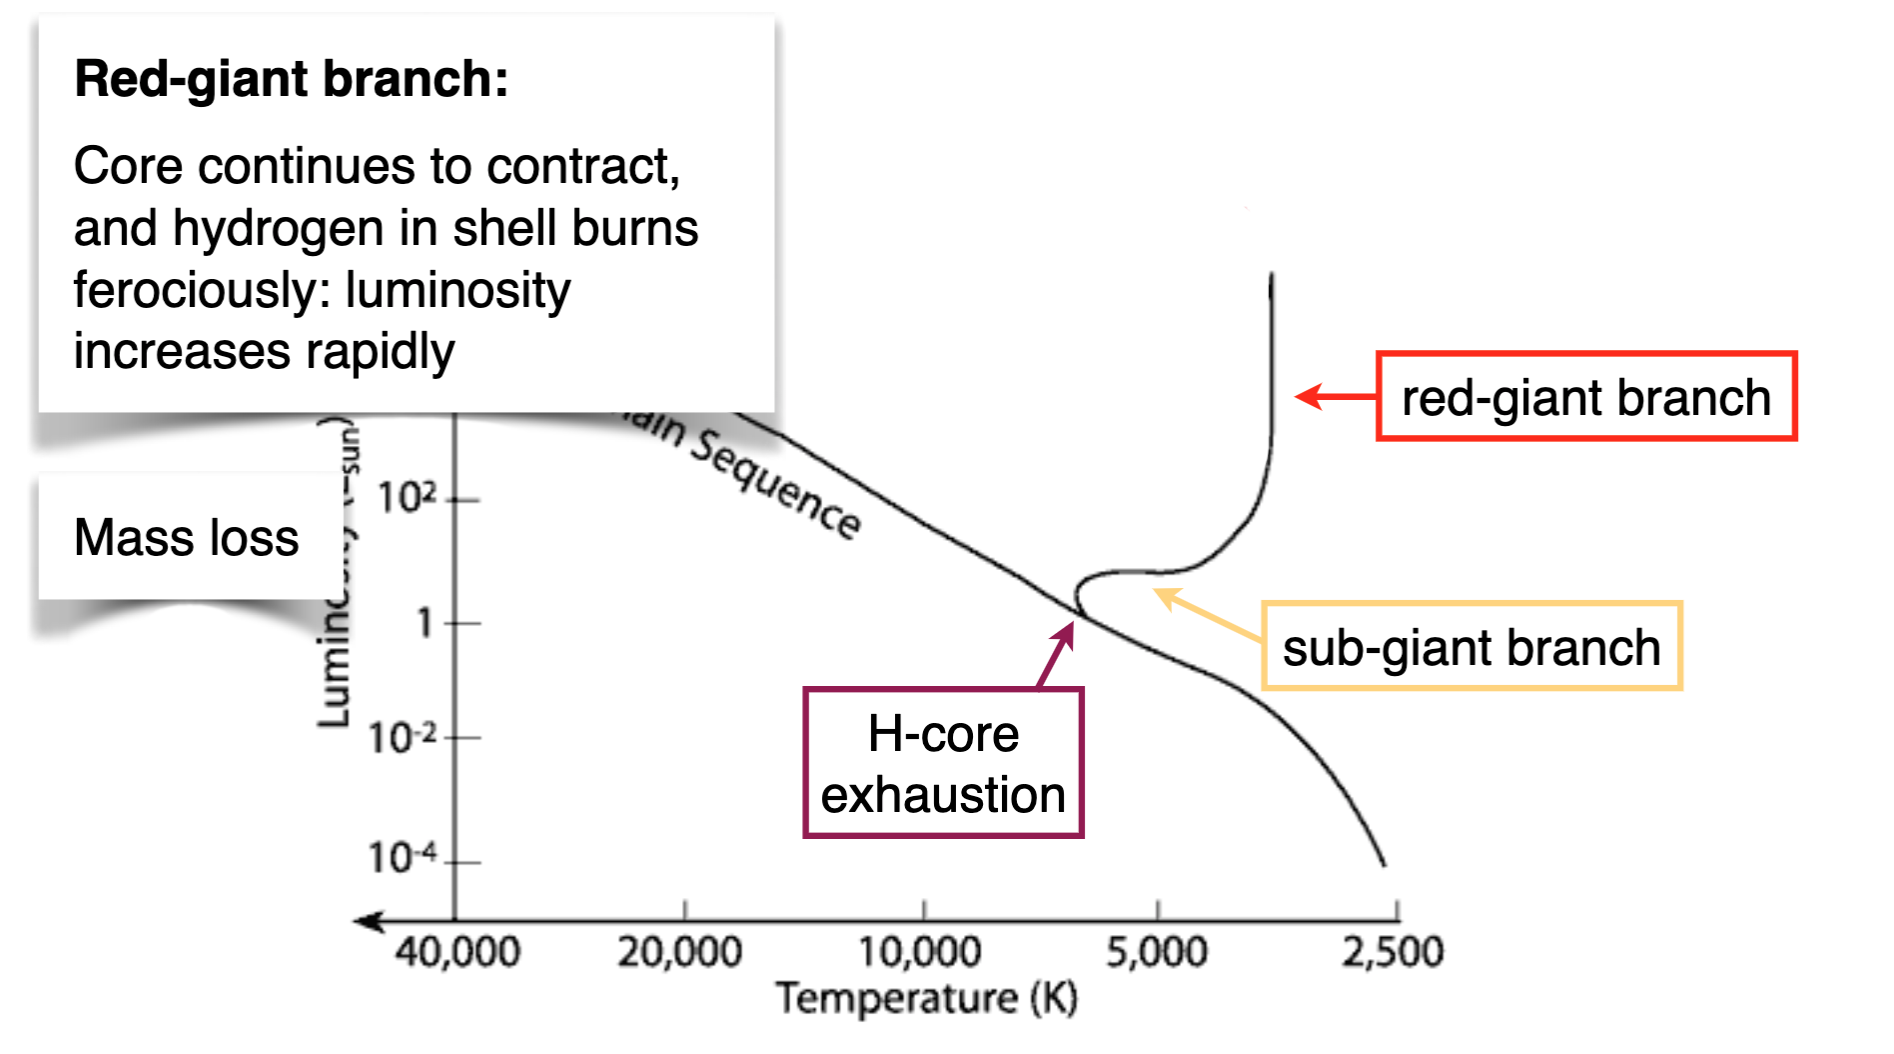
\includegraphics[width=0.66\textwidth]{figs/Screen Shot 2021-09-15 at 9.07.02 AM.png}
    \caption{Red-giant branch.}
    \label{fig:red}
\end{figure}

\begin{figure}
    \centering
    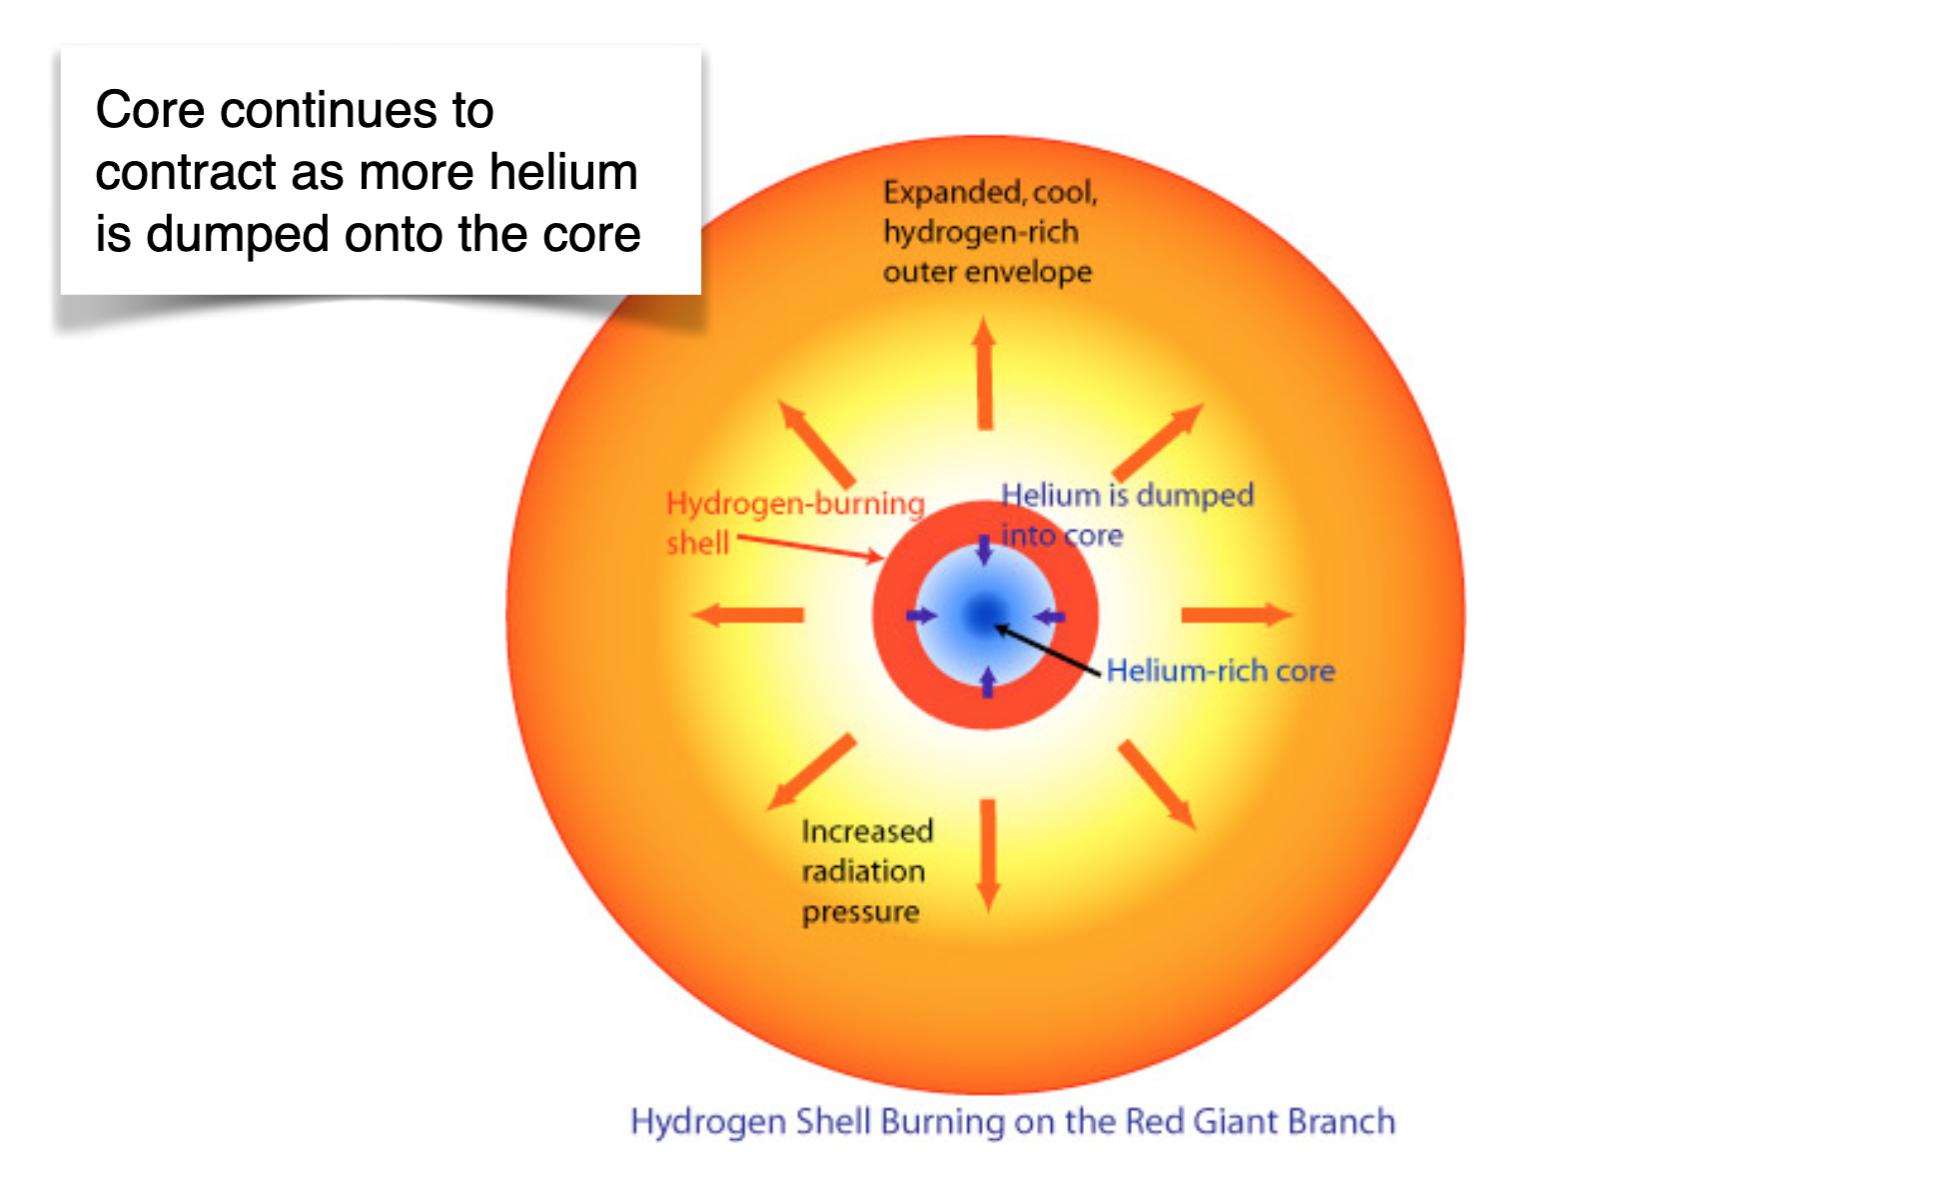
\includegraphics[width=0.66\textwidth]{figs/Screen Shot 2021-09-15 at 9.07.30 AM.png}
    \caption{Red-giant branch 2.}
    \label{fig:red2}
\end{figure}

We then hit the \textbf{helium flash}. This is when the core temperature gets to about $T\sim 10^8$ K. This is so high that helium starts to burn. The core is no longer in free-fall contraction. Boom, we have a burst of energy! The core expands, gravity weakens, and energy production rate goes down. The evolution is to higher temperature and lower luminosity. This is the \textbf{horizontal branch}.

\begin{figure}
    \centering
    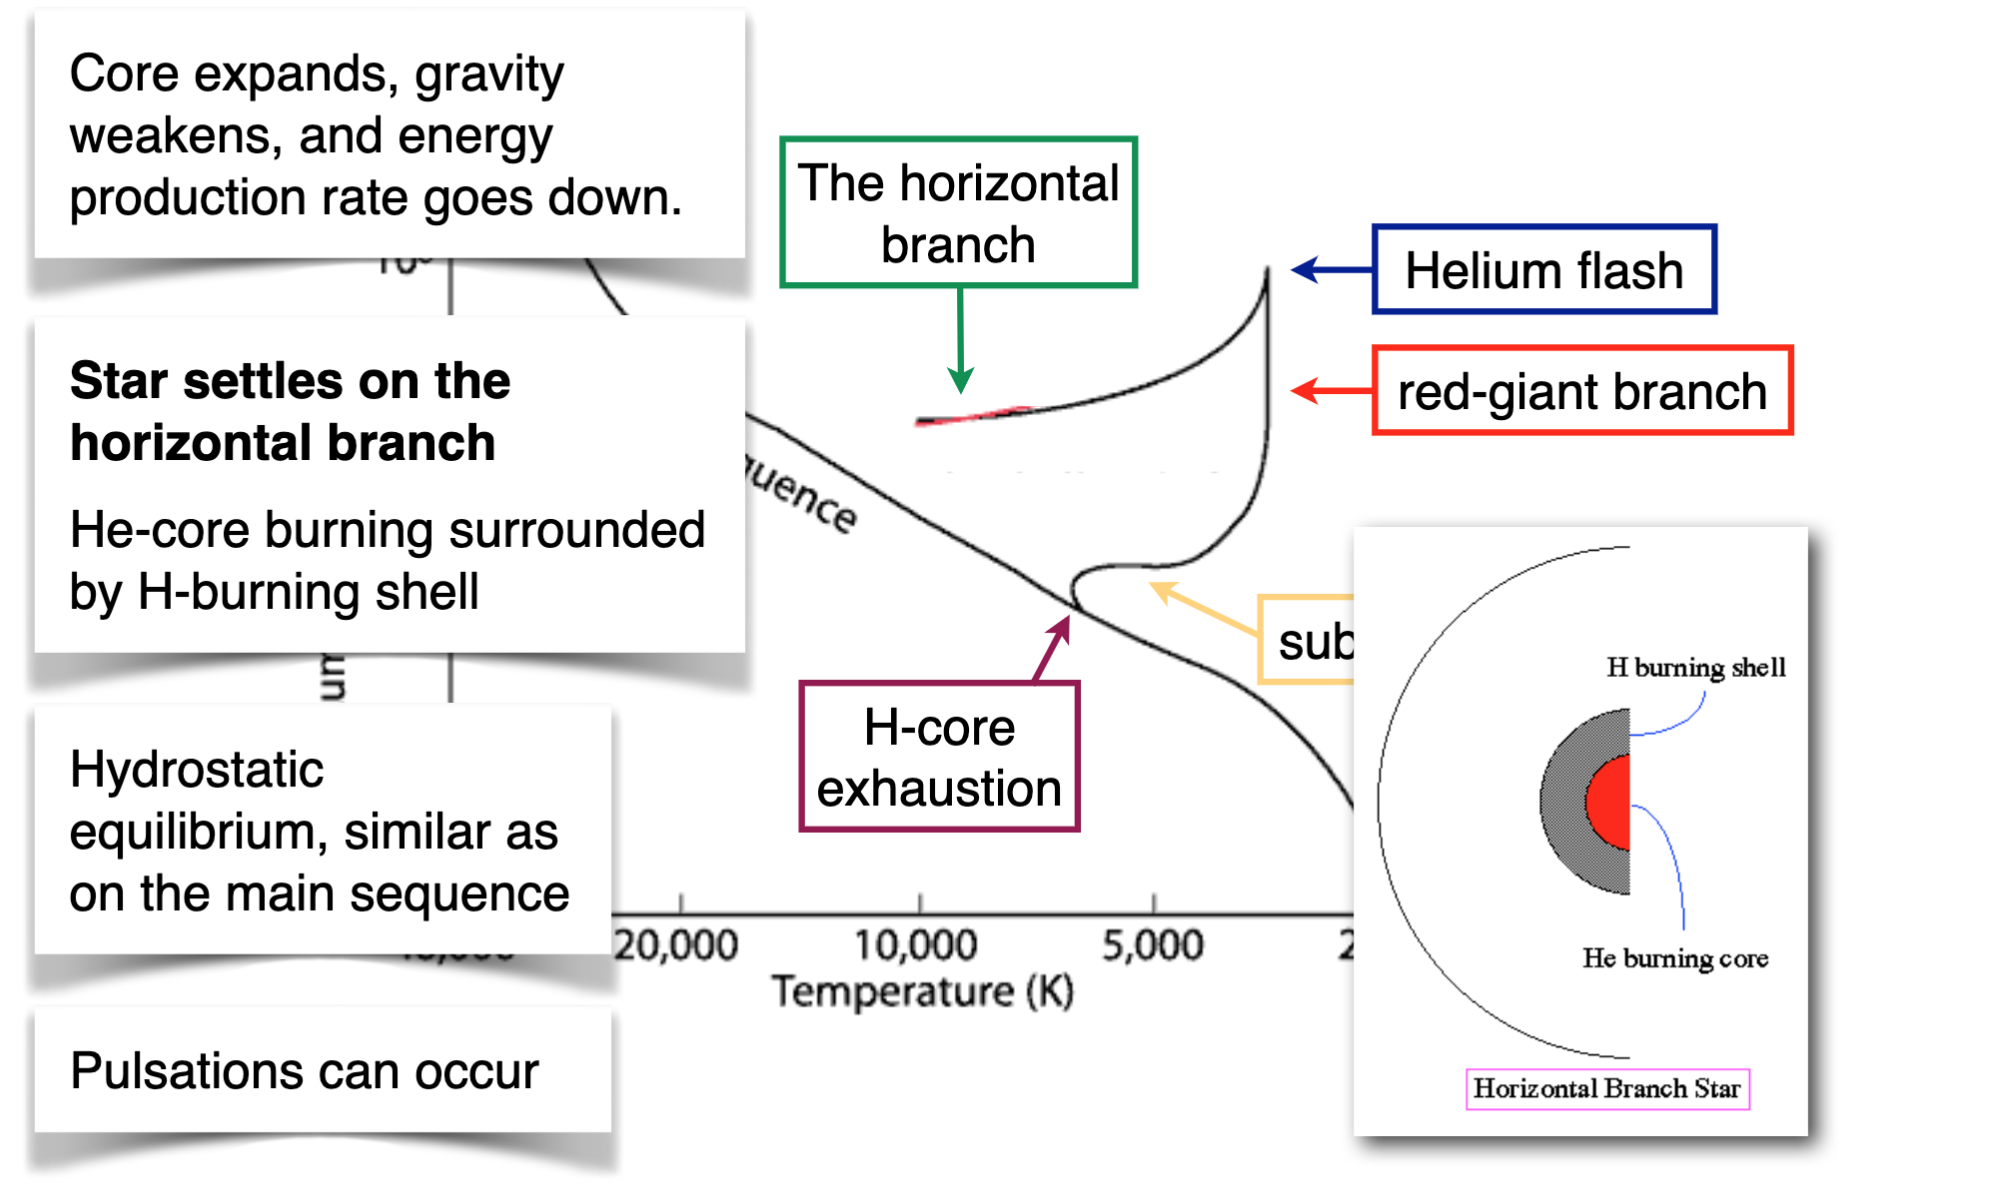
\includegraphics[width=0.66\textwidth]{figs/Screen Shot 2021-09-15 at 9.08.04 AM.png}
    \caption{Horizontal branch.}
    \label{fig:horizontal}
\end{figure}

\textbf{The horizontal branch} is characterized by core helium burning with a surrounding H-burning shell. Tons of details go here, and we don't really fully understand it. This is in hydrostatic equilibrium, however (getting us in the ballpark, sparing the details). This is when pulsations can occur! RR Lyrae are horizontal branch stars. Think of a pot of water with a top on and the pot-top is shaking, allowing for these pulsations. 

\subsubsection{Production of Carbon and Oxygen}

We know how H turns into He. We fuse He with the triple alpha process (helium nucleus is an alpha particle). We basically have:

\begin{equation}
    He_2^4 + He_2^4  \rightarrow Be_4^8 + He_2^4 \rightarrow \gamma + C_6^{12} \rightarrow C_6^{12} + He_2^4 \rightarrow O_8^{16}
\end{equation}

This is what is happening in horizontal branch stars! As you hit the end of the horizontal branch (i.e., not hot enough to fuse helium to carbon and oxygen). Carbon-oxygen core is not burning; the helium burning stars in a shell and the core mass increases. The star mass increases and we are now on the \textbf{asymptotic giant branch}. There is \textbf{a lot} of mass loss here. This is also the \textbf{double shell} burning phase, by the way. 

\subsubsection{Stellar Evolution Tracks}

\begin{figure}
    \centering
    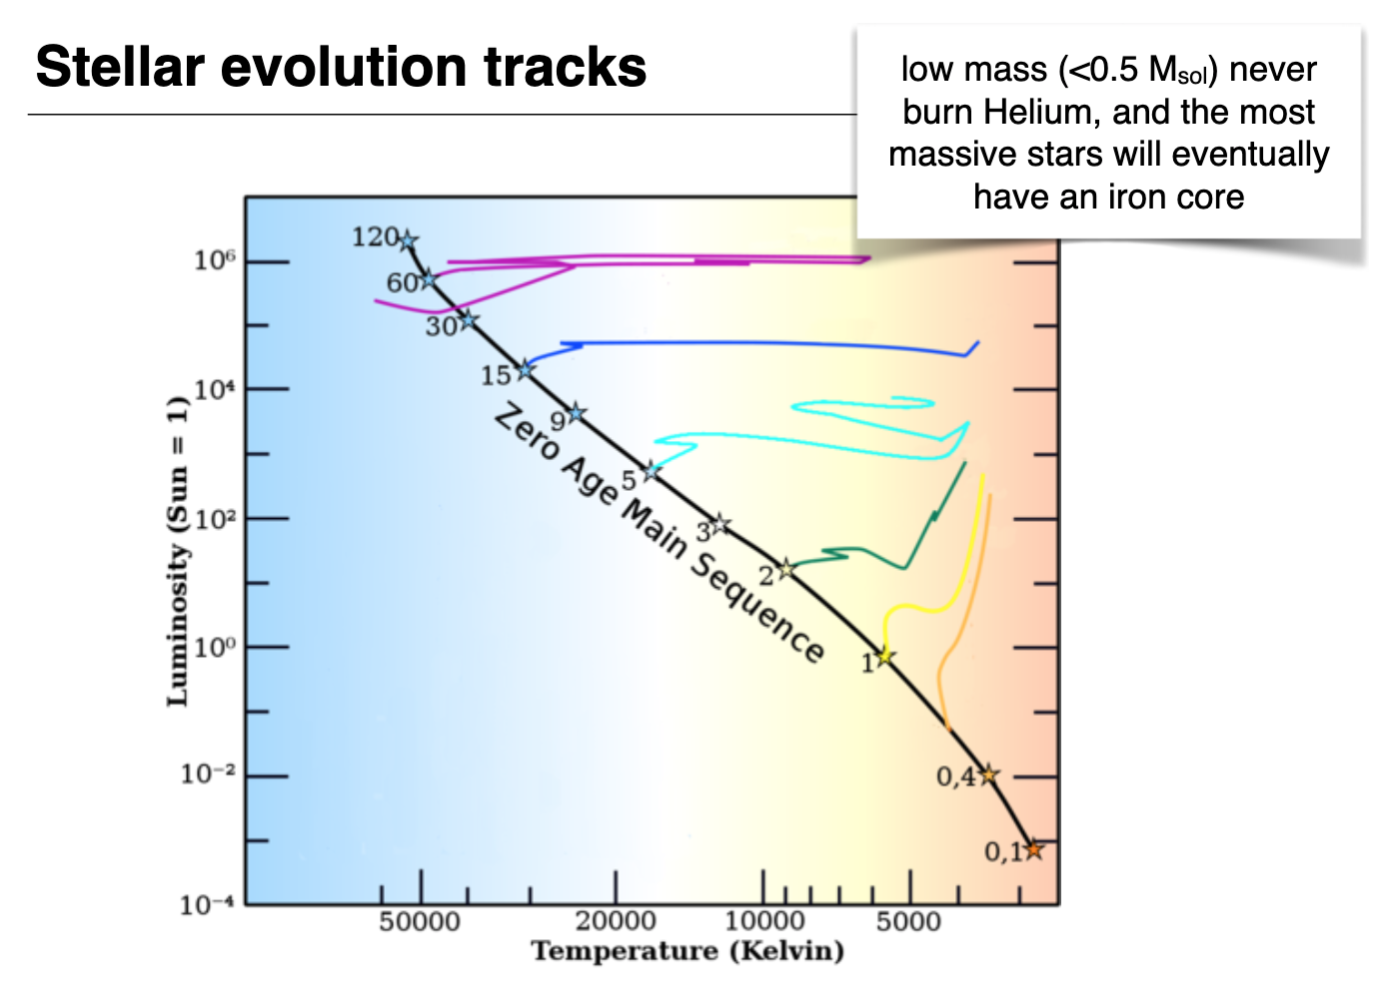
\includegraphics[width=0.66\textwidth]{figs/Screen Shot 2021-09-15 at 9.09.16 AM.png}
    \caption{Stellar evolution tracks.}
    \label{fig:Tracks}
\end{figure}

Evolution of a star at fixed initial mass is a ``track.'' The evolution of high mass stars is crazy! Low mass go mostly vertical, high mass stars bounce around horizontally. 
\subsubsection{Massive Stars}

This is a crazy onion with tons of shells. They burn unbelievably fast, on the order of a few million years. The reactions are really complicated as well. The temperatures are ridiculous high, approaching $T > 10^{9}$ K in order to burn some of the elements. 

\subsubsection{Binding energy per nucleon}

$A$ is the number of nucleons. Less than Fe, energy is liberated via fusion. These reactions are exothermic and energy can be liberated with fusion. Elements heavier than Fe, energy is released with fission and these processes are exothermic.

Iron is most tightly bound and thus cannot fuse. 

\subsubsection{Evolution of a solar mass star}

Eventually becomes a white dwarf which is supported by electron degeneracy pressure. White dwarfs are about the size of the Earth and about a solar mass. 

\subsubsection{Stellar remnants}

Low-to-average mass ends in a white dwarf (up to 7 solar masses or so). Larger stars (between about 7 and 20 [roughly] solar masses) become neutron stars. They are a few solar masses and the size on Manhattan. They are supported by neutron degeneracy pressure. Lastly, the most massive stars become black holes. 

\section{September 15, 2021: Stellar Populations}

\subsection{Ingredients}

\begin{itemize}
    \item \textbf{Initial mass function:} How many stars of a certain mass $M$ are born in a birth cloud $N(M)$? See below for the initial mass function discussion. This gives $N(m)$.
    
    \item \textbf{Isochrones}: Gives the luminosity $L$ and temperature $T$ of a star as a function of mass $M$, age $t$ and metallicity $Z$ of a star. This gives $L(M,t,Z)$ and $T(M,t,Z)$. 
    
    \item \textbf{Spectral library}: Assigns a spectrum to each star using its luminosity $L$, temperature $T$, and metallicity $Z$. This gives $f_\nu(L,T,Z)=f_\nu(M,t,Z)$.
\end{itemize}

\textbf{Simple stellar populations} combine the IMF, isochrones, and stellar spectra to make $\boxed{f_{\nu,ssp}(t,Z)}$.  

\subsection{Initial Mass Function}

\begin{figure}
    \centering
    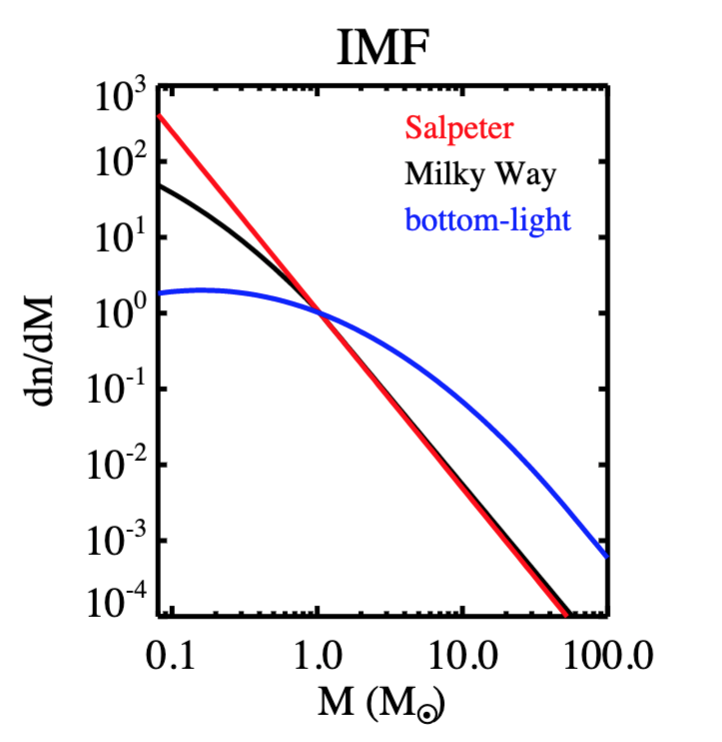
\includegraphics{figs/Screen Shot 2021-09-17 at 9.20.04 AM.png}
    \caption{IMF}
    \label{fig:imf_imf}
\end{figure}

\begin{figure}
    \centering
    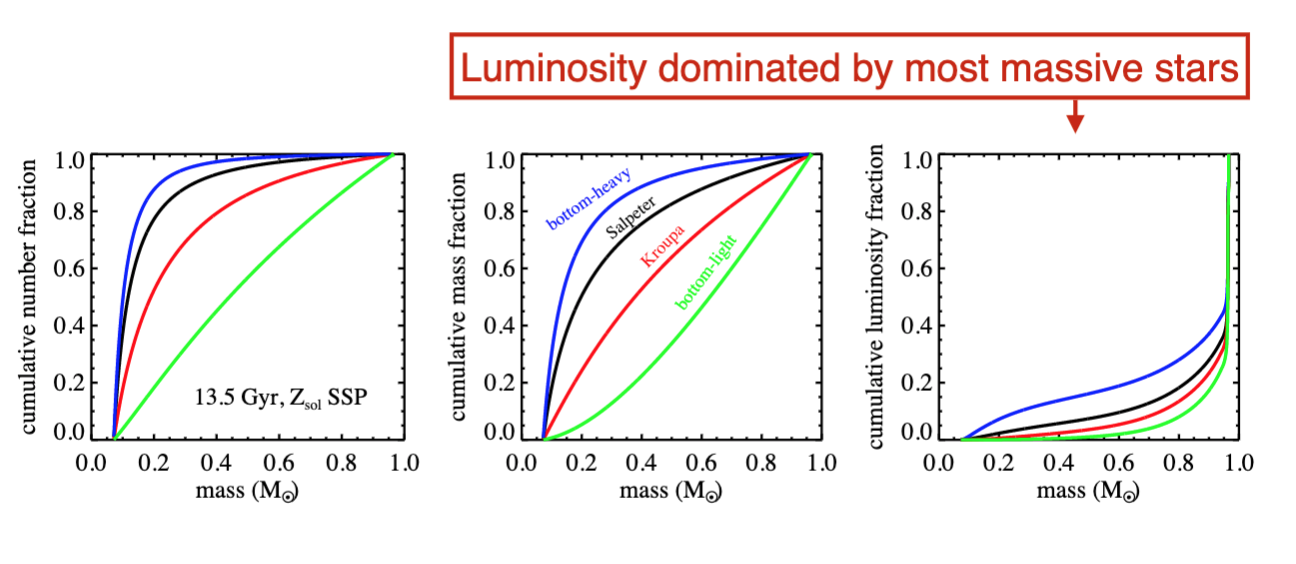
\includegraphics{figs/Screen Shot 2021-09-17 at 9.20.58 AM.png}
    \caption{IMF cont.}
    \label{fig:imfcont}
\end{figure}

This is the distribution of mass \textbf{at birth}, which makes it really difficult to measure. Qualitatively, the Salpeter IMF is a straight line in log-log space:

\begin{equation}
    \xi(m) = \xi_0 M^{-\alpha} \text{, where }\alpha = 2.35
\end{equation}

Sometimes we will see
\begin{equation}
    \xi(m) = \xi_0 M^{-(1+\Gamma)} \text{, where }\Gamma = 1.35
\end{equation}

The $\xi_0$ is a normalization. One question we might have: how many stars exist between two masses?

\begin{equation}
    N = \int_{m_1}^{m_2} \xi(m) \, \mathrm{d} m
\end{equation}

For the Salpeter, we have:

\begin{equation}
    N = \frac{\xi_0}{1.35} \left[\frac{1}{m_1^{1.35}} - \frac{1}{m_2^{1.35}}\right]
\end{equation}

Sometimes you see:

\begin{equation}
    \frac{\mathrm{d}n}{\mathrm{d}m} \propto m^{-2.35}
\end{equation}

\textbf{Note that we are assuming a universal IMF which we will take to be true. This is not necessarily the case.}

\subsection{Evolving a simple stellar population}

\textbf{A galaxy spectrum is dominated by the most massive stars still alive. The galaxy becomes redder and fainter over time, as massive stars die.}

\subsection{Evolution of Color and Mass-to-Light Ratio}

Galaxies become redder in time, and the mass-to-light ration increases in time.

\begin{figure}
    \centering
    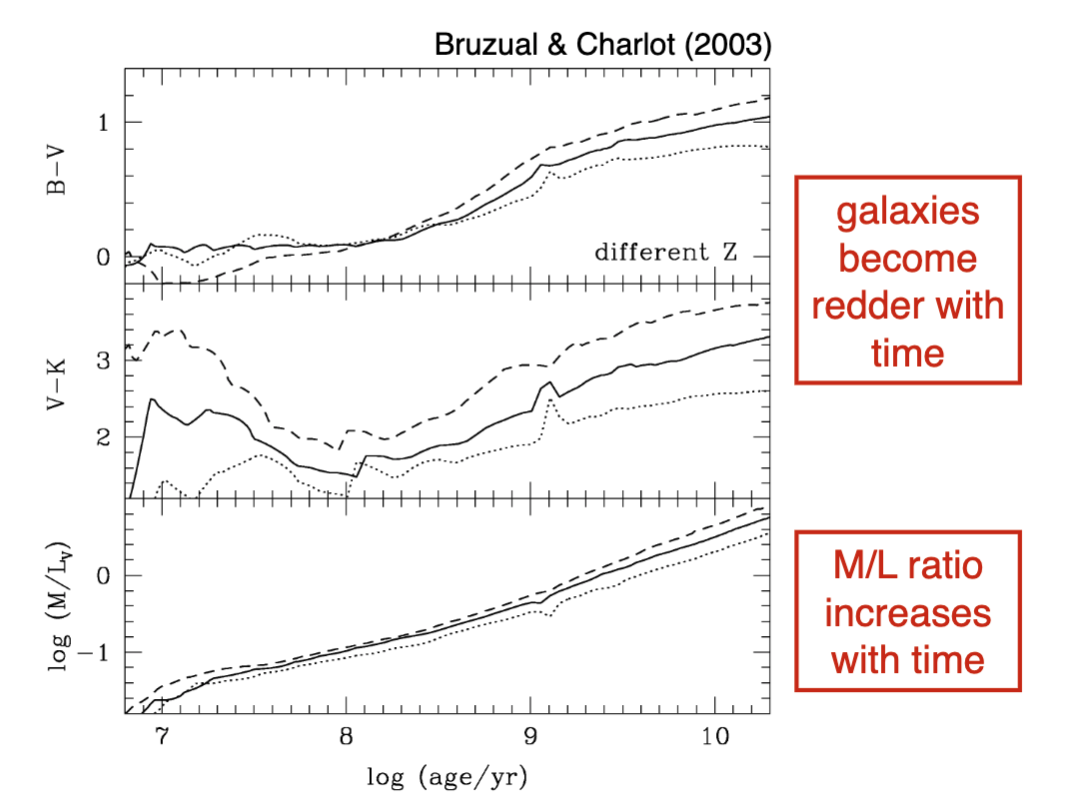
\includegraphics{figs/Screen Shot 2021-09-17 at 9.21.29 AM.png}
    \caption{Evolution of color and M/L ratio.}
    \label{fig:imf}
\end{figure}

\subsection{Dust Attenuation Law}

You typically see $A(\lambda)/A(V)$. This shows that the cross-section/optical depth at bluer wavelengths is larger than at redder wavelengths. In effect, you are losing blue light. 

\textbf{Attenuation} is the net effect of the removal of light. There are many causes, however:
\begin{itemize}
    \item Extinction (how much light is scattered out of the line of sight)
    \item Geometry (what's the geometry of a dust particle, what's the geometry of the galaxy relative to you)
    \item Radiative transfer 
\end{itemize}

We typically describe attenuation with $A_\lambda$:

\begin{equation}
    A_\lambda = \Delta m_\lambda = \left(m - m_0\right)_\lambda
\end{equation}

This is really a magnitude difference (flux ratio) and can also be written as:

\begin{equation}
    F_\lambda = F_{\lambda,0} 10^{-0.4A_\lambda}  = F_{\lambda,0} e^{-\tau_\lambda} \rightarrow A_\lambda = 1.086 \tau_\lambda
\end{equation}

It is also commonly to talk in tewrms of color excess $E(B-V)$:

\begin{equation}
    E(B-V) = A_B - A_V
\end{equation}

\subsection{Dust Attenuation Curve}

\begin{figure}
    \centering
    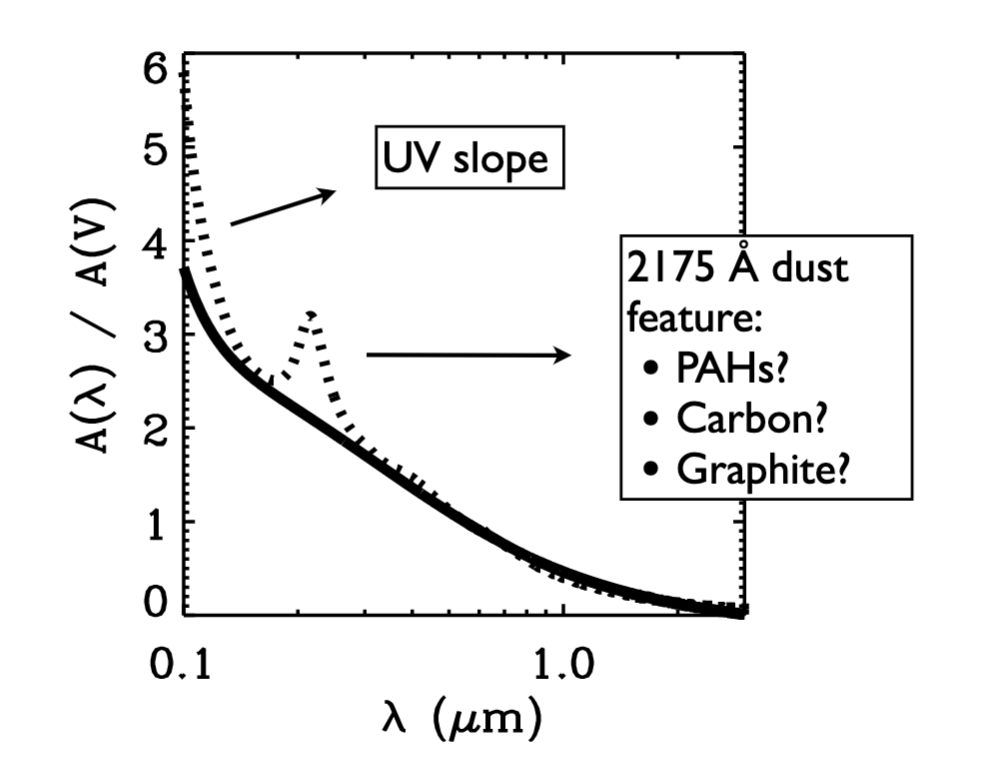
\includegraphics{figs/Screen Shot 2021-09-17 at 9.22.20 AM.png}
    \caption{Dust attenuation law for starburst (solid) and MW. }
    \label{fig:dust_atten}
\end{figure}

You typically see $A(\lambda)/A(V)$ where the center of $V$ is $5500\AA$. We also have the ``attenuation law'' which is:

\begin{equation}
    R_\lambda = \frac{A_\lambda}{E(B-\lambda)}
\end{equation}

Here, $R_\lambda$ is the slope of the attenuation curve. For the MW, this is $R_V = 3.1$. Note that often we assumed a grey atmosphere/slab of material. 

\begin{figure}
    \centering
    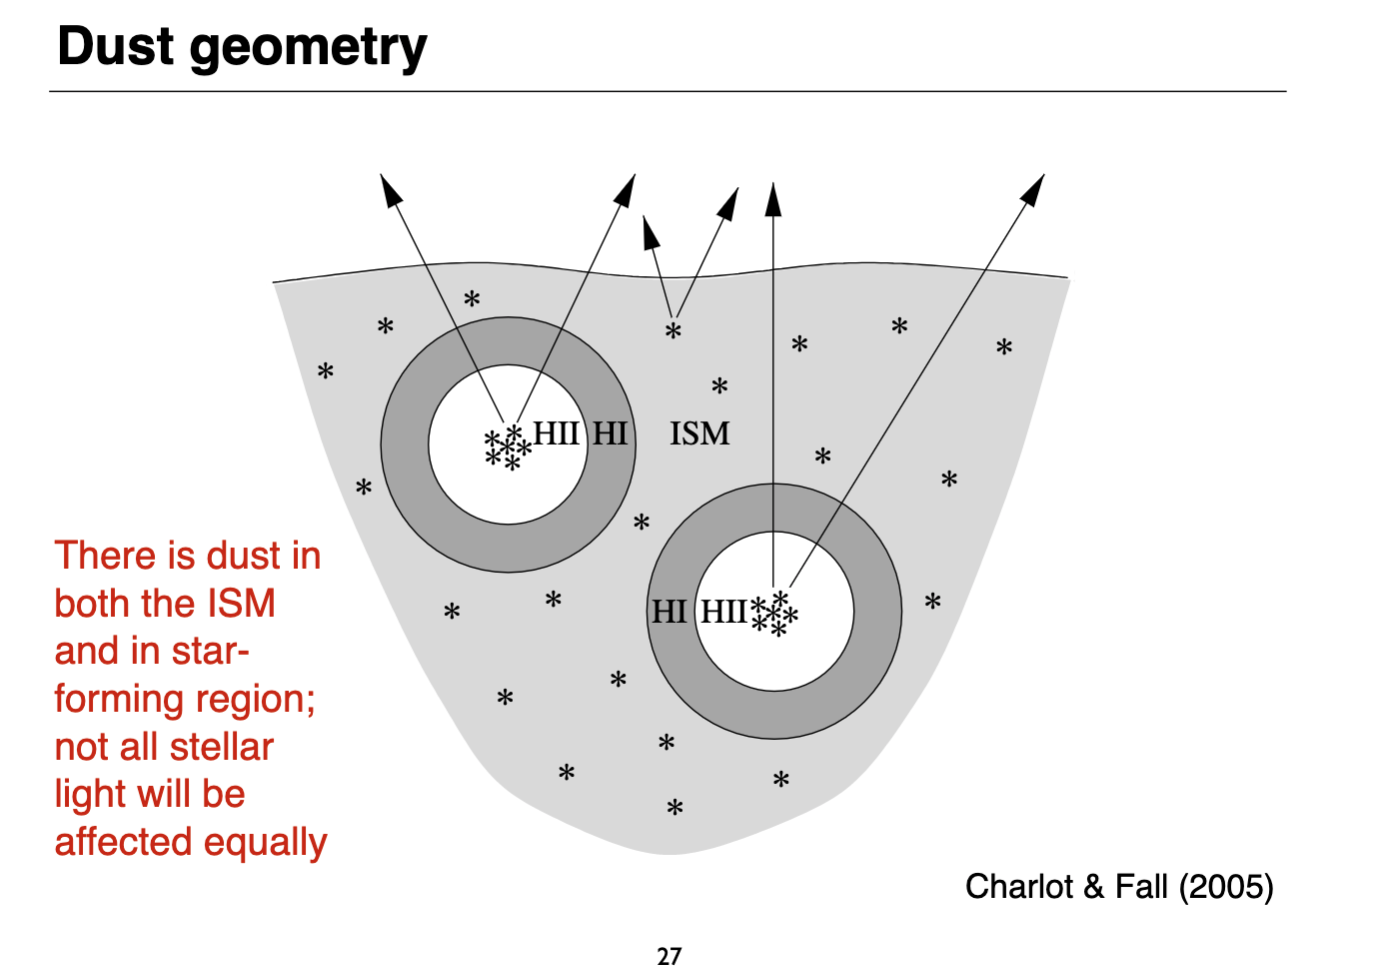
\includegraphics{figs/Screen Shot 2021-09-17 at 9.23.43 AM.png}
    \caption{Dust geometry implications.}
    \label{fig:dust}
\end{figure}

\subsection{Calzetti Law}

Not all attenuation laws are the same. The Calzetti law is popular for starburst galaxies, where the maximum of the attenuation is $3.5$ as opposed to $6$ for the MW. Notice, too, that the MW has the $2175\AA$ bump, which might be caused by:
\begin{itemize}
    \item PAHs
    \item Graphite
    \item Carbon
\end{itemize}

\begin{figure}
    \centering
    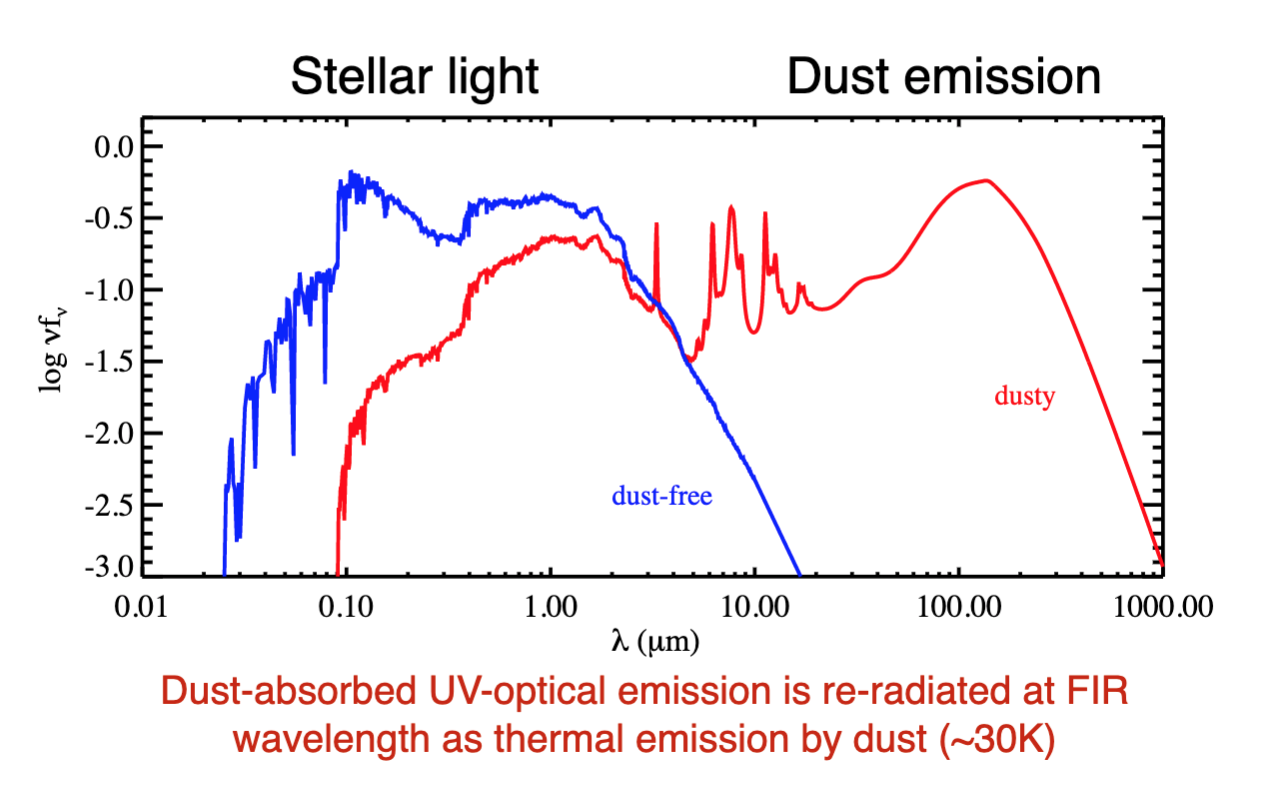
\includegraphics{figs/Screen Shot 2021-09-17 at 9.23.09 AM.png}
    \caption{Sample Galaxy SED. Dust re-radiated at 30K which is warm dust. }
    \label{fig:sedDDD}
\end{figure}

\section{September 17, 2021: Stellar Populations continued}

\subsection{An error from last time...}

Last time, we had used a base $e$ instead of a base $10$ somewhere. Just correcting that. 

\begin{equation}
    A_\lambda = \Delta m_\lambda = \left(m-m_0\right)_\lambda = -2.5\log_{10}\left(\frac{F_\lambda}{F_{\lambda,0}}\right)
\end{equation}

\subsection{Dust Emission Models (Draine and Li, 2007)}

\begin{figure}
    \centering
    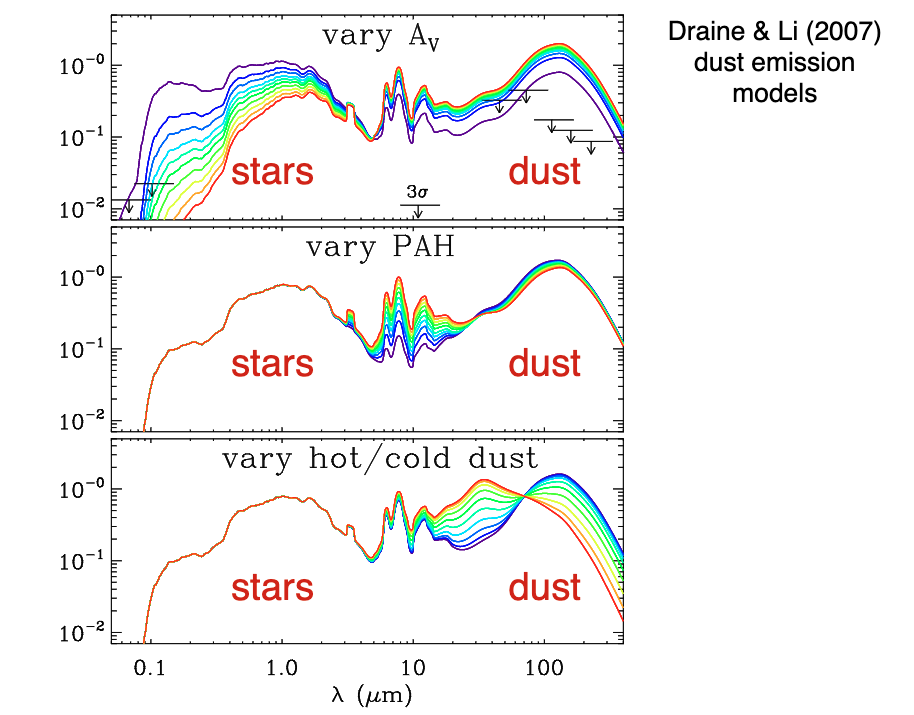
\includegraphics[width=0.66\textwidth]{figs/Screen Shot 2021-09-24 at 9.29.29 AM.png}
    \caption{Varying $A_V$ (increasing) dims starlight and increases dust light. Varying PAHs (increasing PAHs) peak near a few microns and cause many features there. Varying dust temperature (increasing temperature) peaks to smaller wavelengths. Note that varying PAH and temperature does not affect the stars that much. }
    \label{fig:dust_emission_variance}
\end{figure}

\subsection{Negative k-correction}

For higher redshifts, the dust peak becomes fainter and shifts to longer wavelengths. However, the flux density at 1mm stays approximately constant and thus is independent of redshift. Because the spectrum won't fade/shift down, the $k$ correction will be negative. 

\begin{figure}
    \centering
    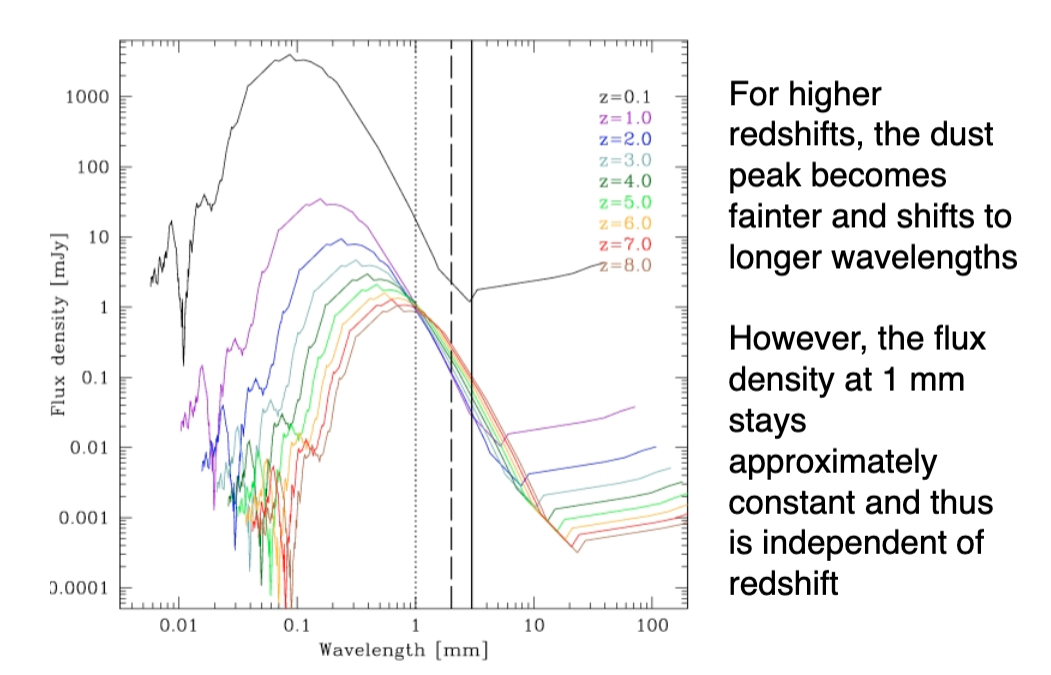
\includegraphics[width=0.66\textwidth]{figs/Screen Shot 2021-09-24 at 9.29.50 AM.png}
    \caption{Negative K-correction}
    \label{fig:negK}
\end{figure}

\subsection{Simple Stellar Populations}

For an SSP, we can write down the flux:

\begin{equation}
    f_{SSP}(t,Z) = \underbrace{\int_{M=m_{lo}}^{M=m_{up}(t)}}_\text{integrate over masses} \underbrace{f_\text{star}\left[T_{eff},\log g(M), t, Z\right]}_\text{flux of a star}\underbrace{\Phi(M)}_\text{IMF}\, \mathrm{d}M
\end{equation}

What are those integration limits? Well $m_{lo}$ is the lowest mass star possible (about $0.08$ solar masses). Higher mass stars die off and thus it is a function of time. Also notice that we are assuming the IMF is a function of mass alone. This is \textbf{controversial}.

\subsection{Star formation history of a simulated galaxy}

\begin{figure}
    \centering
    \includegraphics[width=0.66\textwidth]{figs/Screen Shot 2021-09-24 at 9.31.17 AM.png}
    \caption{SFR of arbitrary galaxy.}
    \label{fig:galsfrarb}
\end{figure}

Broadly, star formation rises rapidly, reaches a peak near $z\sim1$, and then declines toward the present. There are wiggles over time, too, which might be bursty events. 

Instead, we typicall adopt a simplified ``parametrized'' star-formation rates (histories). It is usually parametrized by a smooth function. First, we have a \textbf{falling star formation history/exponential decay}:

\begin{equation}
    SFR \propto e^{-t/\text{0.1 Gyr}} 
\end{equation}

This is popular because it's a one-parameter model! This is also called a $\tau$ model.

Next, we have the \textbf{delayed exponential}:

\begin{equation}
    SFR \propto te^{-t/\tau}
\end{equation}

There is one other parametrization, called a \textbf{rising star formation history}:

\begin{equation}
    SFR \propto t
\end{equation}

And a rising-tau model:

\begin{equation}
    SFR \propto e^{t/\tau}
\end{equation}

\subsection{Star formation and enrichment history}

The increase in metallicity over time depends on the star formation history.

\begin{figure}
    \centering
    \includegraphics[width=0.66\textwidth]{figs/Screen Shot 2021-09-24 at 9.31.57 AM.png}
    \caption{Caption}
    \label{fig:sfr_Z}
\end{figure}

\subsection{Fractional contribution to the total flux}

\begin{figure}
    \centering
    \includegraphics[width=0.66\textwidth]{figs/Screen Shot 2021-09-24 at 9.32.16 AM.png}
    \caption{Fractional contribution to the total flux question.}
    \label{fig:frac}
\end{figure}

Which one has a rising and a falling star formation history?

In a star forming galaxy, the main sequence always dominates. In a rising history, it's \textbf{always} dominated by young luminous stars. This makes the right side rising.

The left side shows that the other weird blue stars dominate instead of blue main sequence stars. This means that larger fractional contributions from post-MS evolution for a falling history. 

\textbf{This plot is important!}

\subsection{Fractional contribution to the total flux for a star forming galaxy}

\begin{figure}
    \centering
    \includegraphics[width=0.66\textwidth]{figs/Screen Shot 2021-09-24 at 9.32.53 AM.png}
    \caption{Fractional contribution 2.}
    \label{fig:frac2}
\end{figure}

Even though $60 M_\odot$ stars are luminous, they are RARE. Thus, star forming galaxies are really characterized by $\sim 10-20 M_\odot$ stars and not \textbf{super-massive} stars. 

\subsection{Light-weighted age as a function of wavelength}

\begin{figure}
    \centering
    \includegraphics[width=0.66\textwidth]{figs/Screen Shot 2021-09-24 at 9.33.28 AM.png}
    \caption{Light-weighted age as a fucntion of wavelenght.}
    \label{fig:lam_age}
\end{figure}

The age that we measure is dependent on our wavelength, since everything if light-weighted. In the infrared, we are sensitive to older populations and thus get closer and closer to the real mass-weighted age. This \textbf{shows the importance of multi-wavelength observations}. It also shows how bad UV obsevrations are at predicting galaxy ages. Also note that the light-weighted age only asymptotes to the mass-weighted age. 

\subsection{Nebular Emission}

One thing we have totally neglected is the effect of nebular emission, which is one of the main ways that we see star-formation in young galaxies. 

\subsection{Complex Stellar Population}

\begin{equation}
    f_{csp}(t) = \int_{t^\prime=0}^{t}\int_{Z=0}^{Z_{max}} \left[SFR(t-t^\prime) P(Z,t-t^\prime) f_{ssp}(t^\prime,Z) e^{-\tau(t^\prime)} + Af_{dust}(t^\prime,Z)\right] \, \mathrm{d}t^\prime \, \mathrm{d} Z
\end{equation}

where $t^\prime$ is the age of the population, $P$ is the metallicity distribution function, $f_{ssp}$ is the integral we had before, $e^{-\tau(t)}$ is an extinction term from dust, and the last term $Af_{dust}$ represents dust emission (with $A$ being a normalization to ensure energy conservation).

Computationally, this is a very annoying calculation to do. 

\subsection{Fitting broadband photometry}

\begin{figure}
    \centering
    \includegraphics[width=0.66\textwidth]{figs/Screen Shot 2021-09-24 at 9.34.14 AM.png}
    \caption{Need full SED to break degeneracies.}
    \label{fig:Z_degen}
\end{figure}

\begin{figure}
    \centering
    \includegraphics[width=0.66\textwidth]{figs/Screen Shot 2021-09-24 at 9.34.40 AM.png}
    \caption{Full spectrum SED.}
    \label{fig:fullsed}
\end{figure}

\subsection{Fitting Spectra without parametrizing the SFH}

\subsection{Uncertainties in the stellar population modeling}

\subsection{Thermally pulsing AGB phase}

These molecular features are imparted because of the AGB star. These are super bright and thus dominate the spectrum. The timescales over which they change their spectra can be short, too (days)! 

\subsection{Challenges of SPS Modeling}

\begin{itemize}
    \item Degeneracies between age and metallicity
    \item SPS models are not perfect; various stages of stellar evolution are poorly understood (AGB, HB, Wolf-Rayet stars, binary evolution, convection, rotation, etc)
    \item Dust law, initial mass function, and star formation history usually assumed
    \item Massive stars with low $M/L$ will dominate the spectra
    \item Etc. 
\end{itemize}

\begin{figure}
    \centering
    \includegraphics[width=0.66\textwidth]{figs/Screen Shot 2021-09-24 at 9.35.27 AM.png}
    \caption{Challenges.}
    \label{fig:Challenges}
\end{figure}


\section{September 22, 2021: Gas and Star Formation}

\subsection{IMF Completion}

We had forgotten a few things. The total mass from an IMF is given by:

\begin{equation}
    M_\star = \int_{m_1}^{m_2} m \xi(m) \,\mathrm{d}m
\end{equation}

An equivalent expression for luminosity:

\begin{equation}
    L_\star = \int_{m_1}^{m_2} L(m) \xi(m) \,\mathrm{d}m
\end{equation}

One other thing, related to the stars...what about the lifetime on the main sequence?

\begin{equation}
    \tau \propto \frac{M}{L} \rightarrow \tau = 10^{10} \frac{M}{L}
\end{equation}

Let's explicitly state something about star formation rates, too. Mathematically, a star formation rate is defined as:

\begin{equation}
    \text{SFR} = \frac{\mathrm{d}M}{\mathrm{d}t} = \dot{M}
\end{equation}

For example, a $\tau$ model is:

\begin{equation}
    \frac{\mathrm{d}M}{\mathrm{d}t} = Ce^{-t/\tau}
\end{equation}

\subsection{Star formation in the nearby Universe}

\begin{figure}
    \centering
    \includegraphics[width=0.66\textwidth]{figs/Screen Shot 2021-09-24 at 3.31.02 PM.png}
    \caption{Starbursts vs. Normal Galaxy}
    \label{fig:starbs}
\end{figure}

At local $z$, roughly $3/4$ of the star formation happen in normal spiral galaxies. The rates range from 0 to a few solar masses per year.

The other quarter of star formation is taking place in star burst galaxies. These have SFRs from a few to $\sim1000$ solar masses per year. 

Stars form in giant molecular clouds (GMCs). They are roughly $10^5$ to $10^6$ solar masses. They extend over a few tens of parsecs, and they have temperatures near $10$ Kelvin. 

We eventually get cold enough that molecules form. Thus the outsides of clouds are less dense than the insides. Outside of the cloud, hot stars pound the surface with radiation (lots of \textbf{self-shielding} interior). There's molecular hydrogen, too, which protects from dissociation of molecules. Eventually gravity takes over, and you form a star!

\begin{figure}
    \centering
    \includegraphics[width=0.66\textwidth]{figs/Screen Shot 2021-09-24 at 3.32.28 PM.png}
    \caption{GMCs}
    \label{fig:GMCs}
\end{figure}



\subsection{Mass function of dense cores in GMCs (Alves+2007)}



Star formation is very inefficient. For a couple of solar masses of stars, you need a TON of gas to make that happen. 

\begin{figure}
    \centering
    \includegraphics[width=0.66\textwidth]{figs/Screen Shot 2021-09-24 at 3.33.05 PM.png}
    \caption{GMC mass function.}
    \label{fig:gmcmass}
\end{figure}

\subsection{Jeans Mass and Cloud Fragmentation}

If you balance gravity against the ideal gas law, you can get the Jeans mass!

The \textbf{Jeans mass}:

\begin{equation}
    M_J \propto \frac{T^{3/2}}{\rho^{1/2}}
\end{equation}

The cloud collapses if the mass of the cloud is greater than the Jeans mass:

\begin{equation}
    M_{CLOUD} > M_J \rightarrow \text{COLLAPSE!}
\end{equation}

In details:

\begin{equation}
    \underbrace{\rho a}_\text{accel.} = \underbrace{-\frac{dP}{dr}}_\text{pressure force per volume} - \underbrace{\frac{GM_r}{r^2}\rho}_\text{gravity per volume}
\end{equation}

There are two phases, roughly. This is summarized in the figure and lists. \textbf{In phase one...}:

\begin{itemize}
    \item Photons can easily escape
    \item $T\sim$ constant (isothermal)
    \item Gravity force / volume $\propto \frac{M^2}{R^5}$
    \item Pressure force / volume $\propto \frac{MT}{R^4}$
    \item For constant $T$, gravity wins: keeps collapsing
\end{itemize}

\textbf{In phase two...}:

\begin{itemize}
    \item Clouds become too dense for photons to escape
    \item Adiabatic: $T\propto \frac{M^{2/3}}{R^2}$
    \item Pressure force increases $\propto \frac{M^{5/3}}{R^6}$
    \item Hydrostatic equilibrium
    \item Further collpase using Kelvin-Helmholtz contraction
\end{itemize}

Note that this is all pre main sequence, so KH contraction really is powering at this point. Then, fusion takes over. 

Another useful thing to keep in mind is the \textbf{freefall timescale} which is generally shorter by a few orders of magnitude than the KH timescale:

\begin{equation}
    t_{ff} \propto \frac{1}{\sqrt{G\rho}}
\end{equation}

\begin{figure}
    \centering
    \includegraphics[width=0.66\textwidth]{figs/Screen Shot 2021-09-24 at 3.34.04 PM.png}
    \caption{Cloud collapse.}
    \label{fig:cloud_collapse}
\end{figure}

\subsection{Star formation rate indicators (recipes)}

\begin{figure}
    \centering
    \includegraphics[width=0.66\textwidth]{figs/Screen Shot 2021-09-24 at 3.35.38 PM.png}
    \caption{SFR Indicators.}
    \label{fig:sfr_indicators}
\end{figure}

\textbf{Fundamental question}: My galaxy has massive stars that we cannot necessarily observe. Can we find another indicator that there is recent or ongoing star formation?

Note that none of this works if we don't have O and B type stars since they have UV emission. 

Let's step through SFR indicators.

\subsection{UV Emission}

The UV is really great to see \textbf{massive stars greater than $3\msun$, or so} (main sequence stars with $T \gtrsim 10^{4}$ K with lifetimes of $10-200$ million years. We can use this emission (corrected for dust with $\beta$ slope) can be used to estimate the SFR of a galaxy. 
\begin{figure}
    \centering
    \includegraphics[width=0.66\textwidth]{figs/Screen Shot 2021-09-24 at 3.36.55 PM.png}
    \caption{Correction with $\beta$ slope.}
    \label{fig:beta_slope}
\end{figure}

Also note that $A_{UV} \sim 8 E(B-V)$ so dust can be really damaging. In practice, we use a \textbf{beta index} which is the slope between a far-UV and near-UV channel. The slope is $\beta$. You can assume that $F_\lambda \propto \lambda^\beta$ to correct for the dust. 

We are measuring the very high mass end of the IMF, and then extrapolating to lower and lower masses. This is part of the reason the IMF is so important. 

\textbf{Assumptions}:
\begin{itemize}
    \item Dust assumption for $\beta$ correction.
    \item Need to assume an IMF.
\end{itemize}

If you take the SPS model, correct for dust, and assume an IMF, you get the \textbf{Kennicutt SFR (98)} relations:

\begin{equation}
    \text{SFR} = 1.4\times10^{-28} L_\nu \frac{\text{ergs}}{\text{s}\cdot \text{Hz}}
\end{equation}

where $L_\nu$ is typically over $\lambda = [1500, 2800] \AA$.

\subsubsection{Correction UV Emission using Beta Slope (Meurer+1999)}

The slope in the UV gives you a crude dust correction (at 1600 Angstrom). This is all that is available at high $z$. Lower $z$ has things like more SED points. 

\subsection{Recombination Lines}

\begin{figure}
    \centering
    \includegraphics[width=0.66\textwidth]{figs/Screen Shot 2021-09-24 at 3.37.34 PM.png}
    \caption{Recombination lines as SFR indicator.}
    \label{fig:recomb_lines}
\end{figure}

Balmer emission lines (lower state $n=2$) originate from HII regions and the underlying absorption lines from stellar atmospheres. Only the most massive stars ($\gtrsim 15 \msun$) can ionize the surrounding medium. Thus, UV emission (corrected for dust with $\beta$ slope) can be used to estimate the SFR of the galaxy. 

The continuum is set by all the stars, and the emission lines are due to the most massive stars ionizing the environment. Let's first look at H$\alpha$.

Let's focus on stars with $M>15 M_\odot$, $T \gtrsim 3\times 10^4$ K, and thus only O-type and B0-type stars. 

If you can measure both H$\alpha$ and H$\beta$, we know that H$\alpha$/H$\beta$ = 2.8. If this is different, we need to correct for the dust changing this ratio.

There is an equivalent \textbf{Kennicutt Recipe (98)}:

\begin{equation}
    \text{SFR} = \frac{L(H\alpha)}{1.26\times 10^{41} \frac{\text{erg}}{\text{s}}}
\end{equation}

Note that this is only sensitive to the most massive stars and thus we are incredibly sensitive to the IMF. 

Here are some of the assumptions:

\begin{itemize}
    \item Assume a metallicity.
    \item Dust correction.
    \item IMF is good since we are measuring only the most massive. 
    \item Binary stars can effect this.
    \item Others.
\end{itemize}

\subsection{FIR Emission}

\begin{figure}
    \centering
    \includegraphics[width=0.66\textwidth]{figs/Screen Shot 2021-09-24 at 3.38.29 PM.png}
    \caption{FIR emission as SFR indicator.}
    \label{fig:fir_sfr}
\end{figure}

FIR emission mostly originates from attenuated UV light from massive stars, i.e., it serves as an SFR indicator. In order to catch both the unobscured and obscured star formation acitivity, we need to combined UV and FIR SFRs. 

There's a \textbf{Kennicutt relation}:

\begin{equation}
    \text{SFR} = \frac{L_{FIR}}{2.2\times 10^{43} \frac{\text{ergs}}{\text{s}}}
\end{equation}

One strength of this is that we can probe regions of high extinction.

\subsection{X-ray emission (Menou et al 2012)}

\begin{figure}
    \centering
    \includegraphics[width=0.66\textwidth]{figs/Screen Shot 2021-09-24 at 3.38.58 PM.png}
    \caption{X-ray emission as SFR.}
    \label{fig:xray_Sfr}
\end{figure}

High-mass X-ray binaries have a very short lifetime ($\sim 20$ Myr) and thus their X-ray luminosity also serves as a SFR indicator. 

X-ray observations are hard to get, and thus this is not used that often. 

\subsection{Radio Emission}

\begin{figure}
    \centering
    \includegraphics[width=0.66\textwidth]{figs/Screen Shot 2021-09-24 at 3.39.38 PM.png}
    \caption{Free-free emission window where it is dominant. }
    \label{fig:FreeFree}
\end{figure}

Synchrotron, thermal free-free emission. There is a small, small window where free-free emission dominates. The wavelengths are really long and thus not affected by dust. There are very few radio telescopes measuring near $30$ GHz, and thus this is hard.

If you could do it, this would be the gold standard since there's no dust and coming from HII regions. 

\subsection{Measuring gas surface densities}

HI is diffuse cold case, CO traces stars forming.

We have two phases of gas -- atomic hyodrogen and molecular CO. The total gass surface density is thus $\Sigma_{gas} = \Sigma_{HI} + \sigma_{H_2}$. $H_2$ is really hard to observe, so we end up measuring:

\begin{equation}
    \Sigma_{gas} = \Sigma_{HI} + \alpha_{CO} I_{CO}
\end{equation}

where $\alpha_{CO}$ takes us from $CO$ to $H_2$. 

The total gas content of $HI + CO$ turns out to be a good tracer of dust. Thus, $\alpha$ is calibrated locally and extrapolated outward. 

This is \textbf{metallicity dependent} since clouds are less-shielded.

\subsection{Kennicutt-Schmidt Law (1998)}

There is a really tight correlation between gas surface density and star formation rate. Often written as the \textbf{KS Relation}:

\begin{equation}
    \Sigma_{SFR} \propto \Sigma_{gas}^n, \text{ where } n = 1.4
\end{equation}




\section{September 24, 2021: Gas and star formation, chemical evolution}

\subsection{Group Exercise}

\begin{figure}
    \centering
    \includegraphics[width=0.66\textwidth]{figs/Screen Shot 2021-09-24 at 9.35.27 AM.png}
    \caption{Group exercise.}
    \label{fig:group}
\end{figure}

Imagine we take two measurements in the UV at $1500\AA$ and $2500\AA$ (far and near UV). The SFR is given by:

\begin{equation}
    \dot{m} = C \times L_{UV}
\end{equation}

Well, we first need \textbf{distance} to go from magnitude to a flux. We also need an estimate of the \textbf{dust correction}. This gives us $L_{UV}$. 

The constant comes from theory. How do we get that? We need to assume an \textbf{IMF}, first of all. We also need a \textbf{metallicity} and assumed \textbf{star formation history}. We need a mass-luminosity relation to get an observable, which we can get from isochrones (more generally, stellar evolution model). One last really subtle thing (not as important for the UV), but it's the \textbf{escape fraction} (fraction of photons coming from star). 

This comes down to basically assuming a Salpeter IMF, one metallicity (solar), a constant star formation history, picking a stellar evolution model, and then an escape fraction of $1$. 

If we saw this edge on, we need to trust our dust correction EVEN MORE!

If you could pick one more wavelength to observe, what would you pick and why? It might be best to get FIR measurements so that we can improve our measurement of $\beta$ by seeing how much light is obscured. 

We might also instead measure high mass X-ray binaries. Thus we have an independent handle (aside from O and B stars). Thus we have two different measurements of $\dot{M}$. 

Another common SFR tracer is H$\alpha$. If we wanted to measure the H$\alpha$ SFR of this galaxy, what do we do? We can go to a telescope and put a narrow band filter on our data and sum the entire image. The UV is produced from $M>3M_\odot$, whereas H$\alpha$ is dominated by $M>15M_\odot$ stars. \textbf{Do we expect that the SFRs agree between the X-ray and UV?} In an ideal world, yes they should be the same. However, if we plot the ratio SFR in H$\alpha$ to SFR in UV, we find that the data is a function of stellar mass at low mass galaxies. This tells us that some assumption is being violated, and this is an active part of research. \textbf{Discrepency in H$\alpha$ and UV SFR tracers is huge!}

We can also take observations at the \textbf{free-free} part of the radio spectrum (where synchrotron is small and free-free dominates). This would be a dust-free measurement of the SFR. 

\subsection{Gas components of a galaxy}

The easiest gas component of a galaxy to measure is HI from the $21$ cm line. HI doesn't get dense enough on its own, so stars really form from $H_2$ (molecule hydrogen). This can get colder and thus denser (because pressure decreases due to temperature). $H_2$ only has a quadrupole moment because it's symmetric. This is \textbf{really weak}, and happens around $\lambda \sim 30 \mu m$. Observing $H_2$ directly is really, really difficult. Instead, we observe CO, which is easily observed. We observe CO near $\lambda \sim 2.6$ mm. We want to know:

\begin{equation}
    \Sigma_{gas} = \Sigma_{H_2} + \Sigma_{H_I} 
\end{equation}

This is also written as:

\begin{equation}
    \Sigma_{gas} = \alpha_{CO} I_{CO} + \Sigma_{H_I}
\end{equation}

Really, we can measure $I_{CO}$ from the telescope and make assumptions on what $\alpha_{CO}$ is. Often, you do not really get a clean measurement.

Instead, you infer the gas content from the dust content. The dust traces the gas, so sometimes this is written as:

\begin{equation}
    \Sigma_{gas} = \underbrace{\delta_{GDR}}_\text{gas-to-dust ratio} \Sigma_{dust} = \alpha_{CO} I_{CO} + \Sigma_{HI}
\end{equation}

We can infer $\delta_{GDR}$ to infer a value of $\alpha_{CO} I_{CO}$.

\begin{figure}
    \centering
    \includegraphics[width=0.66\textwidth]{figs/Screen Shot 2021-09-24 at 9.35.27 AM.png}
    \caption{Looking at HI only, we don't see strong correlation. If we have CO only, the same is true. However, $HI+CO$ is very nicely correlated with gas surface density. }
    \label{fig:coHI_rel}
\end{figure}

\subsection{CO to H2 Conversions}

\begin{figure}
    \centering
    \includegraphics[width=0.66\textwidth]{figs/Screen Shot 2021-09-24 at 9.35.27 AM.png}
    \caption{This has a metallicity dependence because at low metallicity, we expect less dust. }
    \label{fig:alpha_co_z_dependence}
\end{figure}

\subsection{Kennicutt-Schmidt Law}

\begin{equation}
    \Sigma_{SFR} \propto \left(\Sigma_{gas}\right)^n, \text{ where } n =1.4
\end{equation}


\begin{figure}
    \centering
    \includegraphics[width=0.66\textwidth]{figs/Screen Shot 2021-09-24 at 9.35.27 AM.png}
    \caption{Kennicutt-Schmidt relation. Extremely famous.  Relates star formation rate to gas density. What is going on in nature to tell us this correlation?}
    \label{fig:KSR}
\end{figure}

\subsection{KS Law Explanations}

One of the things we discussed was the gas consumption timescale (efficiency factor between gas conversion to stars). It turns out efficiency varies galaxy-to-galaxy. There are three theories.

\begin{itemize}
    \item Efficiency should be constant (wrong). 
    \item \textbf{Theory 1: Free Fall Collapse}: Star formation rate is proportional to gas density and free-fall time: $SFR \propto \frac{\rho}{t_{ff}} \propto \rho \sqrt{G\rho} \propto \rho^{3/2} \propto n^{1.5}$. This is close to Kennicutt-Schmidt! This was first posited in $92$ by Larsen. 
    \item \textbf{Theory 2: Orbital Argument}: Maybe the star formation rate scales with the dynamical (orbital time) of a galaxy. The result is $\Sigma_{SFR} = 0.017 \Sigma_{g} \Omega_{g}$. Paper is 1997 from Elmegreen and Silk. 
    \item \textbf{Theory 3: Molecular Gas Formation is Tough}: Maybe what varies is the ability to \textbf{make} gas. Maybe really $\Sigma_{SFR} \propto \Sigma_{H_2}$, and then we need to figure out how a galaxy can produce $\Sigma_{H2}$ and with what efficiency. Paper by Krumholz (with review in 2014). The corollary of this is that really low metallicity galaxies don't have CO, but they have stars! \textbf{At low metallicity, CO formation is not good and thus our story falls apart! Everyone has molecular hydrogen. $\Sigma_{H2}$ is probably just varying a lot! Lots of theories for why.}
\end{itemize}

\begin{figure}
    \centering
    \includegraphics[width=0.66\textwidth]{figs/Screen Shot 2021-09-24 at 9.35.27 AM.png}
    \caption{Efficiency is more complicated. There is no one efficiency in galaxies. }
    \label{fig:efficiency_epxl}
\end{figure}


\subsection{The star formation law in atomic and molecular gas}

THINGS team finds:

\begin{equation}
    \Sigma_{SFR} = 10^{-2.1} \Sigma_{H2}{1.0}
\end{equation}

\begin{figure}
    \centering
    \includegraphics[width=0.66\textwidth]{figs/Screen Shot 2021-09-24 at 9.35.27 AM.png}
    \caption{Data from THINGS team.  We get the Kennicutt-Schmidt relation really well!}
    \label{fig:THINGS_data}
\end{figure}

\begin{figure}
    \centering
    \includegraphics[width=0.66\textwidth]{figs/Screen Shot 2021-09-24 at 9.35.27 AM.png}
    \caption{More dta}
    \label{fig:krumholz}
\end{figure}

\subsection{Molecular Fraction vs. Gas Surface Density}

Really low surface densities have almost \textbf{NO} $H_2$. Less molecular gas is less star formation. Very tips of spiral arms is not as strong and thus less star formation. Same in dwarf galaxies (cannot pull gas in!). 

\begin{figure}
    \centering
    \includegraphics[width=0.66\textwidth]{figs/Screen Shot 2021-09-24 at 9.35.27 AM.png}
    \caption{Molecular gas fraction and surface density of gas.}
    \label{fig:MORE}
\end{figure}

\subsection{Summary of Today}

\begin{figure}
    \centering
    \includegraphics[width=0.66\textwidth]{figs/Screen Shot 2021-09-24 at 9.35.27 AM.png}
    \caption{SUMMARY of today.}
    \label{fig:summmmm}
\end{figure}




\section{September 29, 2021: The Circumgalactic Medium}


This probably won't be on the final, nor will there be homework on this! 

The first paper; 1956, ApJ, 124, 20S. Lyman Spitzer speculates ``the possibility of a galactic corona.'' The idea was that there must be a medium that supports the gas cloud showing absorption lines far out in the Galaxy! This corona should be really hot, near $10^4 - 10^6$ K. See reviews by \textbf{Putman, Peek, Joung (2012)} and \textbf{Tumlinson, Peeples, Werk, 2017}.

If a galaxy is the size of a dime, the CGM is the size of the DM halo (about the size of a basketball).

Metals in stars can get recycled to the ISM (and observed with gas phase metallicity), \textit{or} with inflows and outflows to the CGM, with recycling. This mixes everything together in the galaxy! 
\subsection{History of CGM}

\begin{itemize}
    \item 1950s to 1960s: Concept of a galactic corona, disovery of NaI and CaII lines in hot star spectra.
    \item 1980s - 2000s: Emerging effort ot study the CGM and IGM with QSO absorption lines out to $z\sim3$. The CGM/IGM gives rise to strong Ly$\alpha$, metal absorption lines and x-rays. 
    \item 2010s: The installation of Cosmic Origins Spectrograph on HST.
\end{itemize}

\subsection{The Missing Baryons \& Where Are They}

See: Persic and Salucci (1992), Fukugita (1998), Fukugita and Peebles (2004), Shull 2003, Bregman 2007, and Behroozi 2010.

\begin{equation}
    f_b = \frac{M(\text{stars, gas, dust})}{M_b}
\end{equation}

\begin{equation}
    M_b = \frac{\Omega_{b}}{\Omega_{m}} M_{DM}
\end{equation}

\begin{equation}
    \Omega_{b} = 0.0486, \text{ and } \Omega_{m} = 0.308 \text{ (from Planck 2015)}
\end{equation}

It turns out, we are missing a lot of baryons that we expect from $\Lambda$CDM. Turns out we are missing a lot of metals, too! The CGM can help explain this, maybe?

\subsection{General GCM Properties}

The CGM is incredibly diffuse, havivng number densities around $n \in [6\times 10^{-7}, 0.6] \text{cm}^{-3}$. We can plot this as a function of temperature in a  \textbf{phase diagram}.

\subsection{Top 10 Observationally Derived Properties of the CGM (Jessica Werk)}

\begin{itemize}
    \item Large covering fraction of multi-phase ions (We can relate the column density to equivalent width through the curve-of-growth.)
    \item Observations strongly hint that CGM gas is bound to the galaxy halo.
    \item \textbf{The CGM gas contains a substantial fraction of baryons and metals, and its content is somehow modified by whatever process shuts down and fuels star formation in galaxies. The CGM phase structure and dominant physical processes are far from being solved, yet data support a complex shocking and mixing of gas within a galaxy virial radius and dominant processes that vary as a function of halo mass. }
\end{itemize}

\subsection{Curve of Growth}

Relates column density to equivalent width, which have three parts. 

\begin{itemize}
    \item Linear regime with $\tau < 1$
    \item Flat regime where width is insensitive, near $10 < \tau < \tau_{damp}$
    \item Very steep regime where $N\propto W^2$ for larger than $\tau_{damp}$
\end{itemize}

\section{October 6, 2021: Chemical Evolution}

\subsection{Chemical Evolution Outline}

\begin{itemize}
    \item Metallicity definition
    \item Sources of heavy elements
    \item Measuring metals
    \item Chemical evolution models
\end{itemize}

\subsection{Terminology and Things}

In most work, we see something like [X/H]. This means ``the number of atoms in X relative to the number of atoms in hydrogen, with the brackets mean relative to the sun. The most common example is [Fe/H]. This is:

\begin{equation}
    \text{[Fe/H]} = \log_{10} \left(\frac{N(Fe)}{N(H)}\right)_\star - \log_{10}\left(\frac{N(Fe)}{N(H)}\right)_\odot
\end{equation}

There are quantities called mass fractions, $X$, $Y$, and $Z$. $X$ is the mass fraction of hydrogen, $Y$ is the mass fraction of helium, and $Z$ is the mass fraction of metals. What this really means is:

\begin{equation}
    X = \frac{m_{hydrogen}}{m_{total}} = \frac{\rho_{hydrogen}}{\rho_{total}}
\end{equation}

By construction, $X+Y+Z = 1$. 

Another example:

\begin{equation}
    \text{[M/H]} = \log_{10} \left(\frac{N(\text{metals})}{N(H)}\right)_\star - \log_{10}\left(\frac{N(Fe)}{N(H)}\right)_\odot
\end{equation}

We can re-write this:

\begin{equation}
    \text{[M/H]} = \log_{10} \left(\frac{n_m}{n_H}_\star / \frac{n_m}{n_H}_\odot\right) = \log_{10}\left(\frac{(Z/X)_\star}{(Z/X)_\odot}\right)
\end{equation}


In the Sun, we have:

\begin{itemize}
    \item $X_\odot$ = 0.734
    \item $Y_\odot$ = 0.25
    \item $Z_\odot$ = 0.016 (controversial -- helioseismology tension!)
\end{itemize}

\subsection{Solar Abundance Pattern}

\begin{figure}
    \centering
    \includegraphics[width=0.66\textwidth]{figs/Screen Shot 2021-10-06 at 10.01.16 AM.png}
    \caption{Solar abundance pattern. This is what you should think about when you talk about abundance patterns, but this is not constant for stars!}
    \label{fig:solar_abundance}
\end{figure}

\subsection{Sources of Heavy Elements}

Hydrogen, helium, and lithium are BBN elements.

Stars return substaional fractions of their initial masses to the ISM at the end of their lifetimes through stellar winds and supernovae.

\begin{itemize}
    \item \textbf{Low mass stars} ($M<8M_\odot$): He, C, N, O ejected during AGB phase
    \item \textbf{Massive stars} ($M>8M_\odot$): Produce more O and Mg compared to Fe. Enrich ISM via stellar winds and final explosions as core collapse (Type II) supernovae
    \item Type Ia supernova: C/O white dwarf accretes material from a close companion and explodes once it reaches the Chandresekhar limiting mass. Produces mostly Fe and little O. 
\end{itemize}

Side note: Hydrogen burning stops, contracts, and inert helium core. Then you have hydrogen shell burning as it ascends RGB. Then helium flash stars the horizontal branch, burning helium in the core burning to C, O. Around the core, you have H burning shells. Then you run out of helium, the core is contracting but not burning. This is the AGB. Everytime its stable, you have same luminosity. Unstable is increasing luminosity. Temperature gradients are really steep and thus you have convection. Dredges up carbon and oxygen into the atmosphere, with winds kicking it off. It then becomes a white dwarf.

\subsection{Neutron Capture Elements}

Most heavy nuclei $(A>56)$ are formed by neutron addition onto Fe-peak elements, followed by beta decay. Beta is an electron or a positron. The neutron capture regime is $n > 10^{20}$ neutrons per centimeter cubed. Low density regime is $n < 10^{8}$. Anything between depends on other factors. Rapid process takes place in SN explosions, colliding neutron stars, BH/neutron star mergers, etc. S process mostly occurs in AGB stars and in massive stars in the He burning core and convective C-burning shell, just prior to SN explosion. 

\begin{figure}
    \centering
    \includegraphics[width=0.66\textwidth]{figs/Screen Shot 2021-10-06 at 10.20.30 AM.png}
    \caption{R and S process. Rapid process takes place in SN explosions, colliding neutron stars, BH/neutron star mergers, etc. S process mostly occurs in AGB stars and in massive stars in the He burning core and convective C-burning shell, just prior to SN explosion. S process is responsible for about half of elements larger than iron. Decay timescale is about 15 minutes. }
    \label{fig:R_S}
\end{figure}

\subsection{R vs. S Process Elements}

\begin{figure}
    \centering
    \includegraphics[width=0.66\textwidth]{figs/Screen Shot 2021-10-06 at 10.24.20 AM.png}
    \caption{}
    \label{fig:rs_stability}
\end{figure}

\subsection{Metallicities of galaxies}

You need high resolution spectra to resolve individual lines. Can also measure the temperature, gravity, and metallicity all at the same time. Can you do the same thing for an integrated population of stars? You can get a value, sure, but it will be luminosity weighted and thus dominated by the brightest stars.

Also, doppler broadening in galaxies makes individual measurements impossible. 

\begin{figure}
    \centering
    \includegraphics[width=0.66\textwidth]{figs/Screen Shot 2021-10-06 at 10.30.19 AM.png}
    \caption{For a star forming galaxy, you measure metallicity from an HII region (equivalent width of emission lines, mostly)! This is a tracer of current metallicity. For quiescent galaxies, we have to measure \textbf{stellar metallicities}, not \textbf{gas-phase metallicities}. Generally measure Mg and Fe abundance. \textbf{Reflects ISM metalicities at times the stars were formed. }}
    \label{fig:metallicities_of_galaxies}
\end{figure}

\subsection{Gas-phase metallicities, direct T method}

You have an optically-thin plasma in a high temperature HII region. The takeaway of the below figure, is: In HII regions, the OIII and NII lines are banged on by other elements. This collisionally excites the plasma, which is great because that's temperature! Thus measuring the temperature gives us the oxygen atoms, and then we can get the metallicity.

How do we get temperature? For OIII specifically, if we can measure ratios of transitions (aka Boltzmann distribution measurements) at specific places, there are places sensitive only to temperature. In practice, many of these lines are weak and hard to measurem (like the 4360 line compared to the 5007 line). 

Instead, you measure the 5007 line, and then something else like H$\beta$, giving:

\begin{equation}
    OIII / H\beta \propto n(O) / n(H) \times T^{0.5} \exp{(-28764/T_e)}
\end{equation}

which is unfortuantely dependent on density, which we must assume! This figure shows this phenomenon:

\begin{figure}
    \centering
    \includegraphics[width=0.66\textwidth]{figs/Screen Shot 2021-10-06 at 10.50.13 AM.png}
    \caption{See above.}
    \label{fig:see}
\end{figure}

We get around this with the \textbf{strong line method}:

\begin{figure}
    \centering
    \includegraphics[width=0.66\textwidth]{figs/Screen Shot 2021-10-06 at 10.50.51 AM.png}
    \caption{Combination of strong lines correlated with oxygen abundance and can be used. Really dangerous though because calibration has lots of scatter. }
    \label{fig:strong_Line_method}
\end{figure}

\begin{figure}
    \centering
    \includegraphics[width=0.66\textwidth]{figs/Screen Shot 2021-10-06 at 10.53.21 AM.png}
    \caption{Direct and indirect method comparison. }
    \label{fig:direct_v_indirect}
\end{figure}

\subsection{Quasar Absorption Line Studies}

Light travels through the medium at many different redshifts, and thus we can measure metallicities of gas patches. This is what Lyman-alpha systems (damped) are:

\begin{figure}
    \centering
    \includegraphics[width=0.66\textwidth]{figs/Screen Shot 2021-10-06 at 10.55.26 AM.png}
    \caption{QSO damped lyman-alpha system. The amount of damping is due to the metal in the gas. Then do photo-ionization modeling. }
    \label{fig:lyman_alpha}
\end{figure}

We can also get metals, too:

\begin{figure}
    \centering
    \includegraphics[width=0.66\textwidth]{figs/Screen Shot 2021-10-06 at 10.59.32 AM.png}
    \caption{We can model other lines which are much weaker, but we know redshift from lyman-alpha.}
    \label{fig:lyman_alpha_systems_metals}
\end{figure}


\section{October 8, 2021: Chemical Evolution Continued}

\subsection{Damped Lyman Alpha Systems}

It might be called this because of radiation damping OR because of the shape of the wings. 

\subsection{Chemical Evolution Models, ingredients}

\begin{itemize}
    \item Initial conditions
    \begin{itemize}
        \item Pre-enriched or primordial
        \item Closed box or open system
    \end{itemize}
    \item Birthrate function $B(M,t) = \psi(t) \xi(M)$
    \begin{itemize}
        \item Star formation rate history: $\psi(t) \propto \sigma^{n}$ (KS relation)
        \item Stellar initial mass function $\xi(m)$
    \end{itemize}
    \item Stellar yields
    \begin{itemize}
        \item Core collapse SN yields depend on stellar mass and metallicity
    \end{itemize}
\end{itemize}

\subsection{Closed Box Model Chemical Evolution}

Let's first define some variables. We have:

\begin{itemize}
    \item $\psi(t)$: SFR in solar masses per year
    \item $M_{g}(t)$ : gas mass at time $t$
    \item $M_s(t)$: Stellar mass at time $t$
    \item $M_t(t) = M_g(t) + M_s(t)$: Total mass at time $t$ which is constant
    \item $Z(t)$: fraction of metals in the gas
\end{itemize}

Now, let's discuss initial conditions:

\begin{itemize}
    \item At $t=0$, $M_t(0) = M_g(0)$ \textbf{and} $Z(0) = 0$.
\end{itemize}

We have a few other assumptions:

\begin{itemize}
    \item No gas flow in or out of the system: $\frac{\mathrm{d}M_t}{\mathrm{d}t} = 0$.
    \item Instantaneous recycling approximation -- no delay time between enrichment and recycling to gas reservoir. 
    \item We basically have an IMF with two mass bins: low mass stars keep stellar mass locked up, high mass stars return the mass to the system. (Recycling of material comes \textbf{only} from high mass stars. Low mass stars retain the mass).
\end{itemize}

We can calculate the stellar mass at time $t$:

\begin{equation}
    M_s(t) = \int_0^t \alpha \psi(t^\prime)\mathrm{d}t^\prime
\end{equation}

where $\alpha$ defines the fraction of mass in long-lived stars. Another way to write this same equation:

\begin{equation}
    \frac{\mathrm{d}M_t}{\mathrm{d}t} = \alpha \psi
\end{equation}


We can write down:

\begin{equation}
    \frac{\mathrm{d}\left(M_g Z\right)}{\mathrm{d}t} = \underbrace{-Z \psi}_\text{removal of metals from system} + \underbrace{\left(1-\alpha\right) Z\psi}_\text{contribution to metals from high mass stars (enrichment)} + \underbrace{q \psi}_\text{}
\end{equation}

where $q \equiv \frac{\text{metals returned}}{\text{total mass}}$ ratio of mass in metals returned to that of the total mass at a given time. In other words, at some time $t$ massive stars are returning metals to the system, which has some total mass at time $t$.

We can re-write the left hand side of the equation above:

\begin{equation}
    \frac{\mathrm{d}\left(M_g Z\right)}{\mathrm{d}t} = q\psi - \alpha Z\psi = \psi\left(q-\alpha Z\right)
\end{equation}

Now, we are going to use a little black magic to expand this...

Let's start with \textbf{Equation 1}:

\begin{equation}
    \frac{\mathrm{d}\left(M_g Z\right)}{\mathrm{d}M_s} = \frac{\mathrm{d}\left(M_g Z\right)}{\mathrm{d}t} \frac{\mathrm{d}t}{\mathrm{d}M_{s}} = \psi(q-\alpha Z)\frac{1}{\alpha \psi} = \frac{q}{\alpha} - Z = y-Z
\end{equation}

Here, we define $y\equiv \frac{q}{\alpha}$. We can now define \textbf{Equation 2}, noting that $\mathrm{d}M_g = - \mathrm{d}M_s$:

\begin{equation}
    \frac{\mathrm{d}\left(M_g Z\right)}{\mathrm{d}M_s} = M_g \frac{\mathrm{d} Z}{\mathrm{d} M_{s}} + Z \frac{\mathrm{d}M_{g}}{\mathrm{d}M_s} = -M_g \frac{\mathrm{d}Z}{\mathrm{d}M_g} - Z = - \frac{\mathrm{d}Z}{\mathrm{d}\ln{M_g}} - Z
\end{equation}


Let's equate \textbf{Equation 1} and \textbf{Equation 2}:

\begin{equation}
    y-Z = - \frac{\mathrm{d}Z}{\mathrm{d}\ln{M_g}} - Z
\end{equation}

Let's simplify:

\begin{equation}
    y = - \frac{\mathrm{d}Z}{\mathrm{d}\ln{M_g}}
\end{equation}

Integrate:

\begin{equation}
    \int_0^t \mathrm{d} Z = -y \int_0^t \mathrm{d}\ln{M_g}
\end{equation}

\begin{equation}
    Z(t) - Z(0) = -y\left(\ln{M_g(t)} - \ln{M_g(0)}\right)
\end{equation}

\begin{equation}
    \boxed{Z(t) = -y \ln{\frac{M_g(t)}{M_t}} = - y \ln{F_g(t)}}
\end{equation}

where $F_g$ is the gas fraction at time $t$. 

We end up wanting to observe the metallicity distribution $\frac{\mathrm{d}N}{\mathrm{d}Z}$. 

\subsection{The G-Dwarf Problem: THIS IS PRE-LIM PRIME}

See Dauphas+2005. G-dwarf dominates the solar neighborhood (because they are easy to observe, by number it's actually the M-dwarfs). The crux of the problem is the low metallicity tail that is totally unfit! So, what's the solution to the closed box model?

The main issue is that we are not in a closed box! The big reason it fails is that we have multiple yields, we have recycling (not instantaneous), and inflow/outflow more broadly speaking and not immediately recycling back into the disk. \textbf{The closed box model needs inflows and outflows, as well as non-instantaneous timescales}.

\begin{figure}
    \centering
    \includegraphics[width=0.66\textwidth]{figs/Screen Shot 2021-10-08 at 10.26.28 AM.png}
    \caption{CB model does not reproduce what is observed!}
    \label{fig:g_dwarf_problem}
\end{figure}

\subsection{Mass-metallicity relation}

We can also look at the mass-metallicity relation. The closed box model fails at reproducing the observed trend. The trend is because, as we change galaxy mass, outflow and inflow are different as a function of mass. 

\begin{figure}
    \centering
    \includegraphics[width=0.66\textwidth]{figs/Screen Shot 2021-10-08 at 10.34.28 AM.png}
    \caption{CB model does not reproduce what is observed for mass-metallicity relation as well!}
    \label{fig:mm_cb}
\end{figure}

\subsection{Leaky Box model}

Modifying the instantaneous recycling approximation, as well as adding in inflows and outflows, and we better fit the data. 

\begin{figure}
    \centering
    \includegraphics[width=0.66\textwidth]{figs/Screen Shot 2021-10-08 at 10.42.51 AM.png}
    \caption{Leaky box better fits the data!}
    \label{fig:leaky_box_model}
\end{figure}

\subsection{Gas Accretion over Time}

\begin{figure}
    \centering
    \includegraphics[width=0.66\textwidth]{figs/Screen Shot 2021-10-08 at 10.46.59 AM.png}
    \caption{Gas accretion slows in the nearby Universe. }
    \label{fig:gasacc}
\end{figure}

\begin{figure}
    \centering
    \includegraphics[width=0.66\textwidth]{figs/Screen Shot 2021-10-08 at 10.49.31 AM.png}
    \caption{Cold mode accretion.}
    \label{fig:cold_mode_acc}
\end{figure}

\begin{figure}
    \centering
    \includegraphics[width=0.66\textwidth]{figs/Screen Shot 2021-10-08 at 10.52.12 AM.png}
    \caption{Hot mode accretion goes down with low halo masses.}
    \label{fig:coldvshot_accre}
\end{figure}

\subsection{Observational Constraints on Infall}

\begin{figure}
    \centering
    \includegraphics[width=0.66\textwidth]{figs/Screen Shot 2021-10-08 at 10.54.33 AM.png}
    \caption{Densities are low, temperatures are low, and thus we have a hard time observing inflows. }
    \label{fig:inflow_constraints}
\end{figure}

\subsection{Lyman Alpha Blobs}

\begin{figure}
    \centering
    \includegraphics[width=0.66\textwidth]{figs/Screen Shot 2021-10-08 at 10.58.30 AM.png}
    \caption{La blobs. Best evidence for inflow.}
    \label{fig:Lymanalpha_blobs}
\end{figure}

\subsection{Milky Way Clouds?}

\begin{figure}
    \centering
    \includegraphics[width=0.66\textwidth]{figs/Screen Shot 2021-10-08 at 11.00.55 AM.png}
    \caption{What the heck are these high velocity clouds?}
    \label{fig:hv_clouds}
\end{figure}


\section{October 13, 2021: Chemical Evolution and DM Halos}

\subsection{CC SN Stellar Yields Depend on the Stellar Mass}

\begin{figure}
    \centering
    \includegraphics[width=0.66\textwidth]{figs/Screen Shot 2021-10-13 at 9.45.24 AM.png}
    \caption{CC SN.}
    \label{fig:CCSn}
\end{figure}

\subsection{CC SN Stellar Yields Depend on the Stellar Metallicity}

\begin{figure}
    \centering
    \includegraphics[width=0.66\textwidth]{figs/Screen Shot 2021-10-13 at 9.47.32 AM.png}
    \caption{Nomoto models are common.}
    \label{fig:Nomoto}
\end{figure}

\subsection{Type Ia Supernvoa Delay Time Distribution}

How many go off as a function of when the star formation episode happened. 

\begin{figure}
    \centering
    \includegraphics[width=0.66\textwidth]{figs/Screen Shot 2021-10-13 at 9.49.40 AM.png}
    \caption{Delay time distributions.}
    \label{fig:DTD}
\end{figure}

\subsection{R-process Elements}

\begin{figure}
    \centering
    \includegraphics[width=0.66\textwidth]{figs/Screen Shot 2021-10-13 at 9.51.39 AM.png}
    \caption{These were thought to track Ia SN. Eu tracks more closely with Mg, which we did not predict. \textbf{We don't know the delay time distribution of neutron star mergers at all which give uncertainty}.}
    \label{fig:Rprocesselements}
\end{figure}

\subsection{PRELIMMABLE: Core-Collapse vs. Type Ia Supernovae Enrichment}

\begin{figure}
    \centering
    \includegraphics[width=0.66\textwidth]{figs/Screen Shot 2021-10-13 at 9.54.53 AM.png}
    \caption{Type II SN go off and produce alpha elements (Mg, Oxygen, Carbon, etc) and not Fe. If you look at a star formation episode shortly after it happens, you find a high alpha sequence (enrichment relative to iron). This is because the Ia's have no happened yet and thus have not produced iron. The first Ia goes off a few hundred million years later, and we enrich the ISM with iron. Effectively, this brings down the alpha-to-iron ratio. }
    \label{fig:FeAlphaEnrichment}
\end{figure}

\begin{figure}
    \centering
    \includegraphics[width=0.66\textwidth]{figs/Screen Shot 2021-10-13 at 9.57.30 AM.png}
    \caption{Initial plateau: ``high-alpha sequence.'' Turnover: ``knee.'' Secondary plateau. This is a diagram that basically traces the various enrichments for Type Ia vs. Type II SN. To get high alpha sequence, we need CCSN. This creates a high alpha population into the ISM. At some time, ISM gets enriched with iron and we have a drop-off in the ratio. Then, we settle in equilibrium. Various aspects of this diagram are sensitive to various SPS parameters. More high mass stars means more CC SN and thus high plateau. The exact shape and slope, location, etc., are set by the balance of star formation rate and inflow/outflow.  }
    \label{fig:AlphaFeAbundanceEnrichment}
\end{figure}

\subsection{Examples - Effect of IMF on Alpha-Fe and Fe-H Diagram}

\begin{figure}
    \centering
    \includegraphics[width=0.66\textwidth]{figs/Screen Shot 2021-10-13 at 10.03.33 AM.png}
    \caption{Cyan is more supernova because more high-mass stars.  }
    \label{fig:Examples1}
\end{figure}

\subsection{Examples - Effect of Star Formation on Alpha-Fe and Fe-H Diagram}

\begin{figure}
    \centering
    \includegraphics[width=0.66\textwidth]{figs/Screen Shot 2021-10-13 at 10.04.44 AM.png}
    \caption{Outflows create spread at the down-turn.   }
    \label{fig:Examples2}
\end{figure}

\subsection{Examples - Effect of Inflow and Outflow on Alpha-Fe and Fe-H Diagram}

\begin{figure}
    \centering
    \includegraphics[width=0.66\textwidth]{figs/Screen Shot 2021-10-13 at 10.07.32 AM.png}
    \caption{Effects of inflows and outflows. }
    \label{fig:Examples23}
\end{figure}

\subsection{The Dark Matter Rap}

\subsection{Cold, Warm DM Power Spectrum}

\begin{figure}
    \centering
    \includegraphics[width=0.66\textwidth]{figs/Screen Shot 2021-10-13 at 10.21.42 AM.png}
    \caption{Characteristic distance scale (x) vs power (y) on sky. Solid line is power spectrum for cold dark matter. We mean by ``cold'': no thermal component. It is just a gravitationally interacting point mass, more or less. The energies corresponding to intrinsic kinetic energy. Warm dark matter has a turnover in the power structure, and you lose small scale structure. }
    \label{fig:DarkMatterPowerSpectrum}
\end{figure}

\subsection{Rotation Curves}

\begin{figure}
    \centering
\includegraphics[width=0.66\textwidth]{figs/Screen Shot 2021-10-13 at 10.25.07 AM.png}
    \caption{Vera Rubin!}
    \label{fig:Vera}
\end{figure}

\subsection{Probes for Dark Matter Halos and Halo Shapes}

\begin{figure}
    \centering
\includegraphics[width=0.66\textwidth]{figs/Screen Shot 2021-10-13 at 10.27.20 AM.png}
    \caption{Prolate and oblate haloes. Things tend to be a bit more prolate, by the way. Typical shape: a : b : c = 1 : 0.8 : 0.65}
    \label{fig:DM_halo_shapes}
\end{figure}

\subsection{Dark Matter Halo: A universal density profile}

The NFW Profile is given by:

\begin{equation}
    \rho(r) = \frac{\rho_s}{\frac{r}{r_s}\left(1 + \frac{r}{r_2}\right)^2}
\end{equation}

where $r_s$ is the scale radius of the halo and $\rho_s$ is the density at $r_s$. 

\begin{figure}
    \centering
\includegraphics[width=0.66\textwidth]{figs/Screen Shot 2021-10-13 at 10.28.42 AM.png}
    \caption{NFW Profile.}
    \label{fig:NFW}
\end{figure}

In practice, however, most people talk about the virial radius. This is the effective radius if the halo were a sphere. If we define $r_{vir}$ and $c_{vir} = \frac{r_{vir}}{r_s}$ is the concentration parameter:

\begin{equation}
    \rho_s = \rho_c \delta_{c} \text{, where } \rho_c = \frac{3 H^2(z)}{8\pi G}
\end{equation}

and where $\delta_c$ is the characteristic overdensity. Typically we pick something like $200$ or $500$ times the overdensity. 

\subsection{Halos which form earlier are more concentrated}

\begin{figure}
    \centering
\includegraphics[width=0.66\textwidth]{figs/Screen Shot 2021-10-13 at 10.38.12 AM.png}
    \caption{Late halos are less dense, as a result of looking at simulations. The characteristic overdensity scales well with the formation epoch. The more concentrated ones tend to be less massive. More massive galaxies have lower dark matter concentration parameters. }
    \label{fig:NFW_Over_Time}
\end{figure}


\subsection{Mergers of Dark Matter Halos}

\begin{figure}
    \centering
\includegraphics[width=0.66\textwidth]{figs/Screen Shot 2021-10-13 at 10.40.32 AM.png}
    \caption{Merger trees. Read from bottom to top moving backward in time. }
    \label{fig:Merger_Trees}
\end{figure}

\subsection{Halo growth; mass accretion histories}

\begin{figure}
    \centering
\includegraphics[width=0.66\textwidth]{figs/Screen Shot 2021-10-13 at 10.43.20 AM.png}
    \caption{Assembling more DM over time. More massive haloes form later than low mass halos. }
    \label{fig:masses_}
\end{figure}

\subsection{Halo growth; concentration paramater histories}

\begin{figure}
    \centering
\includegraphics[width=0.66\textwidth]{figs/Screen Shot 2021-10-13 at 10.44.54 AM.png}
    \caption{Same thing can be said for concentration index.  THis has to do with the fact that they accrete more stuff. Low mass are more simple and thus have simple merging histories.}
    \label{fig:c_parmas}
\end{figure}

\subsection{Dark Matter Halo Mergers: A Universal Fitting Form}

\begin{figure}
    \centering
\includegraphics[width=0.66\textwidth]{figs/Screen Shot 2021-10-13 at 10.47.49 AM.png}
    \caption{Immensely important. }
    \label{fig:chungpeimakesanappearance}
\end{figure}

\begin{figure}
    \centering
\includegraphics[width=0.66\textwidth]{figs/Screen Shot 2021-10-13 at 10.48.23 AM.png}
    \caption{Immensely important. More!}
    \label{fig:chungpeimakesanappearance_2}
\end{figure}

\begin{figure}
    \centering
\includegraphics[width=0.66\textwidth]{figs/Screen Shot 2021-10-13 at 10.49.08 AM.png}
    \caption{Immensely important. More!}
    \label{fig:chungpeimakesanappearance_3}
\end{figure}

\begin{figure}
    \centering
\includegraphics[width=0.66\textwidth]{figs/Screen Shot 2021-10-13 at 10.49.36 AM.png}
    \caption{Barley changes.}
    \label{fig:chungpeimakesanappearance_4}
\end{figure}

\subsection{Problems with Cold Dark Matter}

\begin{itemize}
    \item The missing satellite problem
    \item Cusp-core problem
    \item Halos are triaxial, why don't we see evidence for that?
    \item Why are there so many pure disk galaxies?
    \item Too few galaxies in voids?
\end{itemize}

\subsection{Missing Satellites Problem}

There are tons of tiny little halos that are predicted. Where are they?

\begin{figure}
    \centering
\includegraphics[width=0.66\textwidth]{figs/Screen Shot 2021-10-13 at 10.52.27 AM.png}
    \caption{Where the hell are the satellites?}
    \label{fig:missing_satellites}
\end{figure}

Maybe dark matter isn't cold?

\begin{figure}
    \centering
\includegraphics[width=0.66\textwidth]{figs/Screen Shot 2021-10-13 at 10.54.20 AM.png}
    \caption{Maybe the turnover is due to a warm dark matter turn over? Warm models predict different small DM halos. Probably least likely solution.}
    \label{fig:warmdm}
\end{figure}

\subsection{Core vs. Cusp Problem}

\begin{figure}
    \centering
\includegraphics[width=0.66\textwidth]{figs/Screen Shot 2021-10-13 at 10.55.50 AM.png}
    \caption{NFW is universal, but we observe central regions of nearly constant mass density. This has been used against universal mass profiles. Data appeared to have issues, but problem still exists. }
    \label{fig:core_cusp1}
\end{figure}

\begin{figure}
    \centering
\includegraphics[width=0.66\textwidth]{figs/Screen Shot 2021-10-13 at 10.56.13 AM.png}
    \caption{Proposed solution: baryonic effects (primarily SN feedback) can alter the density profile of law-mass dark matter halos. This is called ``unbinding.'' Probably the best explanation right now.  }
    \label{fig:core_cusp2}
\end{figure}

\subsection{Summary of DM Halos }

\begin{figure}
    \centering
\includegraphics[width=0.66\textwidth]{figs/Screen Shot 2021-10-13 at 11.00.43 AM.png}
    \caption{Summary of DM Halos!  }
    \label{fig:DM_summary}
\end{figure}


\section{October 15, 2021: Elliptical Galaxies}

\subsection{Things to Cover}

\begin{itemize}
    \item Profiles
    \item Scaling relations
    \item Shapes
    \item Stellar dynamics
    \item Formation and evolution
\end{itemize}

\subsection{Brightness Profiles}

Remember deVaucouleur's law:

\begin{equation}
    \log_{10}\left(I/I_0\right) = -3.33\left(\left(\frac{r}{r_0}\right)^{1/4}-1\right)
\end{equation}

\subsection{Sersic Profile}

\begin{equation}
    \mu_{ser} = \mu_0 \exp{-\left(r/r_0\right)^{1/4}}
\end{equation}

For $n=1$, we have an exponential. For $n=4$, we get deVaucouleur's law. 

\begin{figure}
    \centering
\includegraphics[width=0.66\textwidth]{figs/Screen Shot 2021-10-15 at 9.59.34 AM.png}
    \caption{Sersic and Exponential Functions }
    \label{fig:sers_exp}
\end{figure}

\subsection{Correlation between n and effective radius}


\begin{figure}
    \centering
\includegraphics[width=0.66\textwidth]{figs/Screen Shot 2021-10-15 at 10.02.06 AM.png}
    \caption{More massive galaxies have higher Sersic indices.  }
    \label{fig:mass_sers}
\end{figure}

\subsection{Core vs. Coreless Ellipticals}

Sersic is not a perfect description.  What causes core or coreless galaxies? Maybe coreless galaxies come from dissipational mergers (gas present)? Disappationless mergers? 

Maybe instead it's binary black hole scouring. 

\begin{figure}
    \centering
\includegraphics[width=0.66\textwidth]{figs/Screen Shot 2021-10-15 at 10.03.42 AM.png}
    \caption{Core and coreless ellipticals.}
    \label{fig:cores_and_coreless_E0}
\end{figure}


\begin{figure}
    \centering
\includegraphics[width=0.66\textwidth]{figs/Screen Shot 2021-10-15 at 10.06.51 AM.png}
    \caption{Black hole core scouring break radius relation. }
    \label{fig:core_radius_black_hole}
\end{figure}

\subsection{Spheroidal and S0 Galaxies}

\begin{figure}
    \centering
\includegraphics[width=0.66\textwidth]{figs/Screen Shot 2021-10-15 at 10.09.11 AM.png}
    \caption{There are definitely more structure in these galaxies compared to early-type galaxies.  }
    \label{fig:spheroidal_galaxies}
\end{figure}

\subsection{Light Profiles of Different Elliptical Populations}

\begin{figure}
    \centering
\includegraphics[width=0.66\textwidth]{figs/Screen Shot 2021-10-15 at 10.10.43 AM.png}
    \caption{Comparing light profiles. }
    \label{fig:light_profiles}
\end{figure}

\subsection{Sersic Index Correlates with Luminosity}

\begin{figure}
    \centering
\includegraphics[width=0.66\textwidth]{figs/Screen Shot 2021-10-15 at 10.12.18 AM.png}
    \caption{Correlation between sersic and luminosity. Core ellipticals are brighter and have higher $n$. S0 bulges are more comparable to coreless ellipticals.  }
    \label{fig:NeedNewLabel}
\end{figure}

\subsection{Spheroidals vs. Ellipticals (The Kormendy Surface Brightness-Radius Relation}

\begin{figure}
    \centering
\includegraphics[width=0.66\textwidth]{figs/Screen Shot 2021-10-15 at 10.14.37 AM.png}
    \caption{Many take aways: spheroidals are much fainter at the same radii. They do not fall on the same relation (they are not ellipticals). }
    \label{fig:klajdlskjlk}
\end{figure}

\begin{figure}
    \centering
\includegraphics[width=0.66\textwidth]{figs/Screen Shot 2021-10-15 at 10.16.56 AM.png}
    \caption{Another way of showing the previous plot. Spheroidals are fainter and larger at fixed magnitude. }
    \label{fig:MoreMoreMore}
\end{figure}

\subsection{Light Profile of Different Populations}

\begin{figure}
    \centering
\includegraphics[width=0.66\textwidth]{figs/Screen Shot 2021-10-15 at 10.23.06 AM.png}
    \caption{Same luminoisty but very different light profiles. }
    \label{fig:light_profile_differences}
\end{figure}

\subsection{Two Distinct Families}

Think back to the Schechter function (composite of many types). We can do the same thing with galaxy luminosity functions:

\begin{figure}
    \centering
\includegraphics[width=0.66\textwidth]{figs/Screen Shot 2021-10-15 at 10.24.40 AM.png}
    \caption{Light profiles separate into two families!}
    \label{fig:twofamiles}
\end{figure}

\subsection{S0 bulges do fall on the elliptical relations}

\begin{figure}
    \centering
\includegraphics[width=0.66\textwidth]{figs/Screen Shot 2021-10-15 at 10.25.33 AM.png}
    \caption{See figures.}
    \label{fig:bulge_on_relation}
\end{figure}

\subsection{Faber Jackson Relation}

Relates velocity dispersion to the absolute magntiude. Brighter is more velocity dispersion.

\begin{figure}
    \centering
\includegraphics[width=0.66\textwidth]{figs/Screen Shot 2021-10-15 at 10.29.44 AM.png}
    \caption{Stellar velocity dispersion and luminosity relation.}
    \label{fig:faber_jackson}
\end{figure}

\subsection{Stellar Velocity Dispersion}

Faster stars are moving around, the wider the lines because of broadening. 

\begin{figure}
    \centering
\includegraphics[width=0.66\textwidth]{figs/Screen Shot 2021-10-15 at 10.30.29 AM.png}
    \caption{This seems to make sense that the Faber Jackson relation exists!}
    \label{fig:faber_jackson_explanation}
\end{figure}

\subsection{The Kormendy Relation}

Correlation between effective radius and surface brightness. 

\begin{figure}
    \centering
\includegraphics[width=0.66\textwidth]{figs/Screen Shot 2021-10-15 at 10.31.51 AM.png}
    \caption{A pretty tight correlation.}
    \label{fig:kormendy_re}
\end{figure}

\subsection{Can we combine the Faber-Jackson relation with the Kormendy relation?}

How do we relate surface brightness, size, and velocity dispersion? Let's introduce the Fundamental Plane to relate $\mu$, $\sigma$, and $r_e$:

\begin{figure}
    \centering
\includegraphics[width=0.66\textwidth]{figs/Screen Shot 2021-10-15 at 10.33.08 AM.png}
    \caption{The Fundamental Plane.}
    \label{fig:fundamental_plane2}
\end{figure}

\begin{figure}
    \centering
\includegraphics[width=0.66\textwidth]{figs/Screen Shot 2021-10-15 at 10.34.56 AM.png}
    \caption{The Fundamental Plane projected.}
    \label{fig:fundamental_plane_3d}
\end{figure}

\subsubsection{Fundamental Plane in SDSS}

\begin{figure}
    \centering
\includegraphics[width=0.66\textwidth]{figs/Screen Shot 2021-10-15 at 10.35.34 AM.png}
    \caption{The Fundamental Plane projected in different ways.}
    \label{fig:fundamental_plane_many_projections}
\end{figure}

One thing to note: the scatter in the bluer bands of the Fundamental Plane. Indeed it is largely stellar population effects driving the scatter in the relations. Age and metallicity effects are driving the scatter, and these effects are least sensitive at redder wavelengths. \textbf{These are almost always stellar population and dust problems}.

Does the Fundamental plane exist over redshifts? Yes, but the constants will change. 

\section{October 20, 2021: Elliptical Galaxies}

\subsection{Fundamental Plane}

Faber Jackson relation and Kormendy relation give you the Fundamental Plane. We can actually write down the equations explicitly:


\textbf{The Fundamental Plane:}
\begin{equation}
    \boxed{L \propto \sigma_{v,0}^{2.65} r_e^{0.65}}
\end{equation}

\begin{equation}
    r_e \propto \sigma_{v,0}^{1.24} I_e^{-0.82}
\end{equation}

where $\mu = -2.5\log_{10}\left(I_e\right)$. You can also derive the \textbf{Fundamental Plane} from first principles!

\subsection{Fundamental Plane Derivation}

We can start with the \textbf{virial theorem}:

\begin{equation}
    2 \langle K\rangle = -\langle U \rangle
\end{equation}

Re-write the kinetic energy:

\begin{equation}
    2 \langle K \rangle = \langle \Sigma_{i=0}^{N} m_i v_i ^2 \rangle
\end{equation}

The bulk rotation of the galaxy is slow, but the velocity dispersion can be huge! Thus, the important component is the random motion of the stars relative to each other. 

Let's introduce the velocity dispersion $\sigma_v^2$:

\begin{equation}
    \sigma_v^2 = \langle v^2 \rangle - \langle v \rangle^2
\end{equation}

The average of random motions is $0$, and so the second term disappears. we thus get $\sigma_v^2 = \langle v^2 \rangle$. Back to the virial theorem...

\begin{equation}
    2 \langle K \rangle = \langle \Sigma _{i=0}^{N} m_i v_i ^2 \rangle \approx M_\star \sigma_v^2
\end{equation}

What about the potential energy? We have:

\begin{equation}
    U = - C G \frac{M M_\star}{r_e}
\end{equation}

Putting what we have together, we have:

\begin{equation}
    M_\star \sigma_v^2 = - G \frac{M M_\star}{r_e} \rightarrow M = K r_e \sigma_v^2 \text{ where } K \equiv \text{ constants}
\end{equation}

Let's write the surface brightness:

\begin{equation}
    I_e = \frac{F}{\Omega} = \frac{L}{4\pi d^2} \frac{1}{\frac{\pi r_e^2}{d^2}} \propto \frac{L}{r_e^2}
\end{equation}

This is effectively the average surface brightness within $r_e$. Continuing on, we have...

\begin{equation}
    L \propto r_e^2 I_e \rightarrow L \left(\frac{M}{L}\right) \propto r_e \sigma_v^2 \rightarrow r_e^2 I_e \left(\frac{M}{L}\right) \propto r_e \sigma_v^2
\end{equation}

We take this last equation and solve for $r_e$:

\begin{equation}
    r_e \propto \left(\frac{M}{L} \right)^{-1} \sigma_v^2 I_e^{-1}
\end{equation}

Assuming that the mass-to-light ratio is constant, we have:

\begin{equation}
    r_e \propto \sigma_v^2 I_e^{-1}
\end{equation}

The real scaling relation is $r_e \propto \sigma^{1.24} I_e^{-0.82}$
\textbf{The majority of the ``tilt'' of the fundamental plane is due to a changing mass-to-light ratio, but we assumed that it was constant!} This is a good sign that elliptical galaxies are dispersion supported. 

\begin{figure}
    \centering
    \includegraphics[width=0.66\textwidth]{figs/Screen Shot 2021-10-20 at 10.12.59 AM.png}
    \caption{Projections of the FP.}
    \label{fig:fundamental_plane}
\end{figure}

\subsection{Globular Clusters and Dwarf Spheroids}

\begin{figure}
    \centering
    \includegraphics[width=0.66\textwidth]{figs/Screen Shot 2021-10-20 at 10.14.18 AM.png}
    \caption{FP for different populations.}
    \label{fig:fundamental_plane_for_different_galaxies}
\end{figure}

\subsection{Summary so far...}

\begin{itemize}
    \item Elliptical galaxies can be described by a Sersic profile
    \item Elliptical galaxies form a well-defined fundamental plane: the relationship between the effective radius, average surface brightness and central velocity dispersion
    \item The fundamental plane is tilted compared to the virial theorem: due to M/L ratio variations or variations in the structural constant 
    \item The Kormendy and Faber-Jackson relations are projections of the fundamental plane
    \item Dwarf spheroidal galaxies and globular clusters do not fall on the fundamental plane of early-type galaxies; they are not part of the population of early-type galaxies
\end{itemize}

\subsection{Stellar velocity dispersions and dynamics}

See Figure 133.

\begin{figure}
    \centering
    \includegraphics[width=0.66\textwidth]{figs/Screen Shot 2021-10-20 at 10.18.48 AM.png}
    \caption{LOSVDs from rotation asymmetry.}
    \label{fig:asymmetry_rot2}
\end{figure}

Non-Gaussian moments:

\begin{figure}
    \centering
    \includegraphics[width=0.66\textwidth]{figs/Screen Shot 2021-10-20 at 10.21.09 AM.png}
    \caption{van der Marel and Franx 1993.}
    \label{fig:asymmetry_rot}
\end{figure}

\subsection{Velocity Fields}

\begin{figure}
    \centering
    \includegraphics[width=0.66\textwidth]{figs/Screen Shot 2021-10-20 at 10.25.31 AM.png}
    \caption{Velocity fields.}
    \label{fig:vel_fields}
\end{figure}

\subsection{Absorption Line Kinematics}

\begin{figure}
    \centering
    \includegraphics[width=0.66\textwidth]{figs/Screen Shot 2021-10-20 at 10.28.35 AM.png}
    \caption{Continued.}
    \label{fig:continued_stuff}
\end{figure}

\subsection{Stellar Populations in Ellipticals}

\begin{figure}
    \centering
    \includegraphics[width=0.66\textwidth]{figs/Screen Shot 2021-10-20 at 10.35.28 AM.png}
    \caption{High magnesium means lots of Type II before Type Ia and thus is kind of like a clock. We had prompt enrichment (meaning intense star formation rapidly, resulting in many Type II). Core ellipticals are generally older. An old galaxy with high Mg/Fe means. For example, high Mg to Iron means stars formed quickly; high ages mean that it's old. Thus, it formed stars rapidly }
    \label{fig:stellar_pops_elliptical}
\end{figure}

By the time the Type Ia SN are going off, the elliptical has already used its gas and thus cannot continue to iron-enrich the ISM and stars. 

\subsection{Two (historical) formation scenarios}

\begin{figure}
    \centering
    \includegraphics[width=0.66\textwidth]{figs/Screen Shot 2021-10-20 at 10.44.05 AM.png}
    \caption{Two different formation pictures of galaxy formation.}
    \label{fig:gal_form}
\end{figure}

\subsection{Evolution of the IMF}

\begin{figure}
    \centering
    \includegraphics[width=0.66\textwidth]{figs/Screen Shot 2021-10-20 at 10.45.07 AM.png}
    \caption{IMF variations.}
    \label{fig:IMF_variations}
\end{figure}

\subsection{Average SFHs for Low-Z Early-Type Galaxies}


\begin{figure}
    \centering
    \includegraphics[width=0.66\textwidth]{figs/Screen Shot 2021-10-20 at 10.47.43 AM.png}
    \caption{Average SFHs. More massive galaxies formed their stars earlier over a shorter timescale. }
    \label{fig:low_z_ETG_SHF}
\end{figure}

\subsection{Signs of ongoing mergers}

\begin{figure}
    \centering
    \includegraphics[width=0.66\textwidth]{figs/Screen Shot 2021-10-20 at 10.49.36 AM.png}
    \caption{Signs of ongoing mergers.}
    \label{fig:ongoing_merger_histories}
\end{figure}


\subsection{ETGs were smaller at earlier times}

\begin{figure}
    \centering
    \includegraphics[width=0.66\textwidth]{figs/Screen Shot 2021-10-20 at 10.51.16 AM.png}
    \caption{Observed counts can indeed explain size evolution.}
    \label{fig:size_evolution_ETGs}
\end{figure}

\subsection{Inside-Out Growth}

\begin{figure}
    \centering
    \includegraphics[width=0.66\textwidth]{figs/Screen Shot 2021-10-20 at 10.52.15 AM.png}
    \caption{Inside-out.}
    \label{fig:vo4}
\end{figure}

\subsection{A moer realistic formation scenario}

\begin{figure}
    \centering
    \includegraphics[width=0.66\textwidth]{figs/Screen Shot 2021-10-20 at 10.54.40 AM.png}
    \caption{Star formation grows the core. Minor mergers dissipationalessly grow the galaxy later. This can help place galaxies on the fundamental plane, and variety comes from accretion history.}
    \label{fig:vo3}
\end{figure}

\subsection{A two phase model: where and when:}

\begin{figure}
    \centering
\includegraphics[width=0.66\textwidth]{figs/Screen Shot 2021-10-20 at 10.56.54 AM.png}
    \caption{oser2010, low mass halo}
    \label{fig:vo}
\end{figure}

\begin{figure}
    \centering
\includegraphics[width=0.66\textwidth]{figs/Screen Shot 2021-10-20 at 10.59.33 AM.png}
    \caption{oser2010, intermediate mass halo}
    \label{fig:vo2}
\end{figure}

\begin{figure}
    \centering
\includegraphics[width=0.66\textwidth]{figs/Screen Shot 2021-10-20 at 10.57.34 AM.png}
    \caption{many stars were not formed in-situ, but rather accreted and reside in the outskirts. this is high mass}
    \label{fig:outskrts}
\end{figure}

We rely on rapid star formation and accretion later for mass building elliptical galaxies.

\section{October 22, 2021: Disk Galaxies: Characteristics and Scaling Relations}

\begin{figure}
    \centering
    \includegraphics[width=0.66\textwidth]{figs/Screen Shot 2021-10-22 at 9.45.57 AM.png}
    \caption{Pics!}
    \label{fig:diskpics}
\end{figure}

\subsection{Overview}

\begin{itemize}
    \item Componenets
    \item Stellar pops
    \item Bulges
    \item Kinematics
    \item The Tully-Fisher relation
\end{itemize}

\subsection{Disk galaxy surface brightness profile}

\begin{figure}
    \centering
    \includegraphics[width=0.66\textwidth]{figs/Screen Shot 2021-10-22 at 9.46.50 AM.png}
    \caption{SBP of disk galaxies. Not well fit by a single profile. Often assume an exponential. Bulge and disk need to be fit separately.}
    \label{fig:sbp}
\end{figure}

\subsection{GALFIT: Galaxy Profile Fitting}

\begin{figure}
    \centering
    \includegraphics[width=0.66\textwidth]{figs/Screen Shot 2021-10-22 at 9.48.29 AM.png}
    \caption{GALFIT.}
    \label{fig:GALFIT}
\end{figure}

\subsection{Properties along the Hubble Sequence}

\begin{figure}
    \centering
    \includegraphics[width=0.66\textwidth]{figs/Screen Shot 2021-10-22 at 9.51.35 AM.png}
    \caption{Reminder of context.}
    \label{fig:hubble_tuning_fork}
\end{figure}

\subsection{Mass-size relation}

\begin{figure}
    \centering
    \includegraphics[width=0.66\textwidth]{figs/Screen Shot 2021-10-22 at 9.52.30 AM.png}
    \caption{Mass-size relation for galaxies.}
    \label{fig:massiszerelation}
\end{figure}

\subsection{Disk properties}

\begin{figure}
    \centering
    \includegraphics[width=0.66\textwidth]{figs/Screen Shot 2021-10-22 at 9.53.14 AM.png}
    \caption{Older disks are brighter and more massive. They also rotate faster. }
    \label{fig:disk_properties}
\end{figure}

\begin{figure}
    \centering
    \includegraphics[width=0.66\textwidth]{figs/Screen Shot 2021-10-22 at 9.54.20 AM.png}
    \caption{More properties.}
    \label{fig:props}
\end{figure}

\subsection{Color Gradients}

\begin{figure}
    \centering
    \includegraphics[width=0.66\textwidth]{figs/Screen Shot 2021-10-22 at 9.55.24 AM.png}
    \caption{Y-axis is basically telling us age. X-axis can basically be thought of as radius. Bluer stars in the center. Later types are overall bluer. }
    \label{fig:boo}
\end{figure}

\subsection{Classical Bulge vs Pseudo-bulges}

Classical bulges are smoother and they are $\sim$ elliptical galaxies. Pseudo bulges usually live in disk galaxies with spiral structure and nuclear star formation. The light is typically dominated by young stars. Many pseudo bulges rotate, whereas classical bulges often do not.  

\begin{figure}
    \centering
    \includegraphics[width=0.66\textwidth]{figs/Screen Shot 2021-10-22 at 10.02.22 AM.png}
    \caption{Bulges and pseudo-bulges.}
    \label{fig:bulges}
\end{figure}

\subsection{Classical versus pseudo bulges}

\begin{figure}
    \centering
    \includegraphics[width=0.66\textwidth]{figs/Screen Shot 2021-10-22 at 10.04.29 AM.png}
    \caption{Bulges and pseudo-bulges scaling relations. Psuedo bulges have lower $n$, lower magnitude, surface brightness. }
    \label{fig:bulges_relations}
\end{figure}

\begin{figure}
    \centering
    \includegraphics[width=0.66\textwidth]{figs/Screen Shot 2021-10-22 at 10.05.24 AM.png}
    \caption{Motion of velocity fields. Hbeta gives you SFR. }
    \label{fig:NGC3623}
\end{figure}

\subsection{Pseudobulges have central star formation}

\begin{figure}
    \centering
    \includegraphics[width=0.66\textwidth]{figs/Screen Shot 2021-10-22 at 10.07.31 AM.png}
    \caption{24 micron show us hot dust near stars. 24 micron are just redder than AGB but way bluer than cold dust. Dust absorbs the UV photons and re-radiate around 20 micron.}
    \label{fig:dust_in_bulges}
\end{figure}

\subsection{Rotation Curves from Ha}

\begin{figure}
    \centering
    \includegraphics[width=0.66\textwidth]{figs/Screen Shot 2021-10-22 at 10.10.40 AM.png}
    \caption{Offset is due to recession!}
    \label{fig:rot_crves_disks}
\end{figure}

\begin{figure}
    \centering
    \includegraphics[width=0.66\textwidth]{figs/Screen Shot 2021-10-22 at 10.12.15 AM.png}
    \caption{Rubin! Evidence for dark matter. Should drop off, but does not!}
    \label{fig:vera_rubin}
\end{figure}

\subsection{Extent of the stellar and gas disk}

\begin{figure}
    \centering
    \includegraphics[width=0.66\textwidth]{figs/Screen Shot 2021-10-22 at 10.12.59 AM.png}
    \caption{Everything in 21 cm can be converted to gas mass! We can also get the kinematics of the gas. They also go wayyyyyy out, for almost all spirals.}
    \label{fig:21cm_disks}
\end{figure}

\begin{figure}
    \centering
    \includegraphics[width=0.66\textwidth]{figs/Screen Shot 2021-10-22 at 10.14.53 AM.png}
    \caption{More extended HI in M33. }
    \label{fig:b0000m}
\end{figure}

\subsection{Spider Diagram}

\begin{figure}
    \centering
    \includegraphics[width=0.66\textwidth]{figs/Screen Shot 2021-10-22 at 10.18.35 AM.png}
    \caption{Spider galaxy. The contours after subtracting the systemic velocity leaves contours of constant LOS velocity! Usually, the HI is aligned with the major axis. }
    \label{fig:spider_diagram}
\end{figure}

\begin{figure}
    \centering
    \includegraphics[width=0.66\textwidth]{figs/Screen Shot 2021-10-22 at 10.20.34 AM.png}
    \caption{As you go out, the contours will close because you have lower and lower enclosed mass the system.}
    \label{fig:enclosed_mass_gives_circles}
\end{figure}

\subsection{Spider diagrams for complex velocity fields}

\begin{figure}
    \centering
    \includegraphics[width=0.66\textwidth]{figs/Screen Shot 2021-10-22 at 10.23.01 AM.png}
    \caption{M83 is a local starburst galaxy analog. In reality, we have to fit tilted ring models (or warped disk models). This is when the photometric and kinematic axes are not aligned, or the axes are not perpendicular. Lots of reasons for a warp, mostly do to recent interactions. }
    \label{fig:warps}
\end{figure}

\subsection{Measuring vmax from single-dish observations}

\begin{figure}
    \centering
    \includegraphics[width=0.66\textwidth]{figs/Screen Shot 2021-10-22 at 10.26.13 AM.png}
    \caption{Single dish observations cannot really spatially resolve velocity. They use $W_{20}$ to characterize these curves. }
    \label{fig:single_dish_stuff}
\end{figure}

What is this used for? We can still measure Vmax, but that can tell us about the enclosed mass and thus the dark matter.

\subsection{The Tully-Fisher Relation}

This tells us the scaling between the rotational velocity and the absolute magnitude of the galaxy. You end up finding $L \propto V^{4}$ with $\alpha = 3$ to $4$. We can make an argument that gets us close.

\begin{figure}
    \centering
    \includegraphics[width=0.66\textwidth]{figs/Screen Shot 2021-10-22 at 10.30.07 AM.png}
    \caption{Measure HI velocity. Get cepheids for distances in these galaxies. There is a tight correlation between luminosity of disk galaxies and thus its dark matter content (rotational velocity). You find }
    \label{fig:tf_relat}
\end{figure}

\subsection{Tully Fisher Derivation from Virial Theorem}

The empirical version is $L \propto v_{max}^{3.4}$. Let's start with the virial theorem:

\begin{equation}
    2 \langle K \rangle = - \langle U \rangle 
\end{equation}

Following last time:

\begin{equation}
    \langle K \rangle = \frac12 M \langle v^2 \rangle \rightarrow \frac12 C_1 M \langle v_{max}^2 \rangle
\end{equation}

\begin{equation}
    U = -C_2 \frac{G M^2}{r_e}
\end{equation}

We now have:

\begin{equation}
    M C_1 v_{max}^2 = C_2 \frac{GM^2}{r_e} \rightarrow M = \frac{r_e v_{max}^2}{C_1 C_2 G}
\end{equation}

Do the same algebraic trick as last time, multiply by the mass-to-light ratio:

\begin{equation}
    L = \left(\frac{M}{L}\right)^{-1} \frac{r_e v_{max}^2}{C_1 C_2 G}
\end{equation}

We now \textbf{assert a constant mass-to-light} ratio:

\begin{equation}
    L \propto r_e v_{max}^2
\end{equation}

We make another assertion (though it's egregious). Let's say we have an exponential surface brightness profile:

\begin{equation}
    I(r) = I_0 e^{\frac{-r}{r_0}}
\end{equation}

where $r_0 \propto r_e$. Taking this SBP, we find:

\begin{equation}
    L_{tot} \propto 2\pi I_0 r_0^2
\end{equation}

It turns out there is a thing called \textbf{Freeman's Law}, which says there is an approximate constant surface brightness for disk galaxies. Using this as an assertion:

Thus,

\begin{equation}
    L \propto r_0^2 \propto r_e^2 \rightarrow r_e \propto \sqrt{L}
\end{equation}

Returning to before:

\begin{equation}
    L \propto \sqrt{L} V_{max}^2 \rightarrow \boxed{L \propto v_{max}^4}
\end{equation}

\textbf{The Tully-Fisher is powerful for the same reasons as the Fundametnal plane. }

\subsection{The Baryonic Tully Fisher Relation}

\begin{figure}
    \centering
    \includegraphics[width=0.66\textwidth]{figs/Screen Shot 2021-10-22 at 10.45.58 AM.png}
    \caption{Baryonic Tully-Fisher relation. What is the deal with the green points on the left? The green points are the regime of the dwarf galaxies. Remember Kennicutt-Schmidt? In dwarf galaxies, the KS relation does not hold. The green points thus represent the fact that the stars do not represent the total mass of the system. It still is pretty good! For astrophysical studies, masses are often much more useful. }
    \label{fig:BTF}
\end{figure}

\begin{figure}
    \centering
    \includegraphics[width=0.66\textwidth]{figs/Screen Shot 2021-10-22 at 10.48.54 AM.png}
    \caption{Summary of today. }
    \label{fig:summary_today_BTF}
\end{figure}


\section{October 27, 2021: Disk Galaxies and Spiral Structure}

\subsection{Spiral Arms}

\begin{figure}
    \centering
    \includegraphics[width=0.66\textwidth]{figs/Screen Shot 2021-10-27 at 9.51.41 AM.png}
    \caption{The arms appear more defined at longer wavelengths because ongoing star formation is heating the dust and radiating in the infrared. By the time you get to 3.5 micron, you are really tracing old stars. The arms are thus either young.}
    \label{fig:spirals_arms}
\end{figure}

\begin{figure}
    \centering
    \includegraphics[width=0.66\textwidth]{figs/Screen Shot 2021-10-27 at 9.54.24 AM.png}
    \caption{More pretty pictures!}
    \label{fig:more_spiral_arms}
\end{figure}

\begin{figure}
    \centering
    \includegraphics[width=0.66\textwidth]{figs/Screen Shot 2021-10-27 at 9.55.32 AM.png}
    \caption{Dust lanes are generally a bit displaced from the spiral arms. We talk about this later. You do see OB associations which do trace the locus of the spiral arm. Dust lanes are on the inner edge of spiral arms.}
    \label{fig:dust_lanes}
\end{figure}

\subsection{Molecular Gas}

\begin{figure}
    \centering
    \includegraphics[width=0.66\textwidth]{figs/Screen Shot 2021-10-27 at 9.56.27 AM.png}
    \caption{Molecular gas is also offset from the spiral arms as well. Hard to tell, but as we saw before, the CO follows the dust. The little red regions being lit up are where the CO \textit{was}.}
    \label{fig:locus2}
\end{figure}

\subsection{Atomic Gas}

\begin{figure}
    \centering
    \includegraphics[width=0.66\textwidth]{figs/Screen Shot 2021-10-27 at 9.57.28 AM.png}
    \caption{Interesting -- the atomic gas seems to traces the locus of the spiral arms, whereas the other components didn't. Remember that the atomic ga is a reservoir for star formation, but not the site itself of star formation. }
    \label{fig:locus}
\end{figure}

\subsection{Types of Spirals}

\begin{figure}
    \centering
    \includegraphics[width=0.66\textwidth]{figs/Screen Shot 2021-10-27 at 10.00.02 AM.png}
    \caption{Grand design. Caption should be $\sim 10$ percent. }
    \label{fig:Grand_design.}
\end{figure}

\begin{figure}
    \centering
    \includegraphics[width=0.66\textwidth]{figs/Screen Shot 2021-10-27 at 10.00.42 AM.png}
    \caption{Multiple arm spirals.}
    \label{fig:mutli_arm}
\end{figure}

\begin{figure}
    \centering
    \includegraphics[width=0.66\textwidth]{figs/Screen Shot 2021-10-27 at 10.01.23 AM.png}
    \caption{Flocculent spiral. These are the most common type of spiral. }
    \label{fig:flocculent_spiral}
\end{figure}

\begin{figure}
    \centering
    \includegraphics[width=0.66\textwidth]{figs/Screen Shot 2021-10-27 at 10.01.58 AM.png}
    \caption{Least to most common from left to right.}
    \label{fig:more_Tpyes}
\end{figure}

\subsection{Spiral Arm Categories}

\begin{figure}
    \centering
    \includegraphics[width=0.66\textwidth]{figs/Screen Shot 2021-10-27 at 10.03.02 AM.png}
    \caption{Can you identify them?}
    \label{fig:boomboom}
\end{figure}

\subsection{Arm Prominence}

\begin{figure}
    \centering
    \includegraphics[width=0.66\textwidth]{figs/Screen Shot 2021-10-27 at 10.04.48 AM.png}
    \caption{Surface brightness as a function of angle. Note the bottom right. Flocculent are thus more star forming, in general. Grand design, on the other hand, are a bit older. }
    \label{fig:asdasd}
\end{figure}

\subsection{Trailing vs. Leading Spiral Arms}

\begin{figure}
    \centering
    \includegraphics[width=0.66\textwidth]{figs/Screen Shot 2021-10-27 at 10.07.42 AM.png}
    \caption{Note that the spiral arms can be decoupled from the bulk rotation of the galaxy. }
    \label{fig:trailing_leading}
\end{figure}

\begin{figure}
    \centering
    \includegraphics[width=0.66\textwidth]{figs/Screen Shot 2021-10-27 at 10.12.41 AM.png}
    \caption{Projection effects. We can look for differential obscuration.  }
    \label{fig:proj_eff}
\end{figure}

\subsection{Arm Fragments}

Most basic explanation of the formation of spiral arms is differential rotation.

\begin{figure}
    \centering
    \includegraphics[width=0.66\textwidth]{figs/Screen Shot 2021-10-27 at 10.16.44 AM.png}
    \caption{Perturbation shears into a spiral arm. This works well for flocculent patterns.}
    \label{fig:arm_fragment_theory}
\end{figure}

\begin{figure}
    \centering
    \includegraphics[width=0.66\textwidth]{figs/Screen Shot 2021-10-27 at 10.22.11 AM.png}
    \caption{Overwinding problem: Eventually, the arms should fragment and dissolve. Does not predict long-lived arms though we still observe that. Really this is saying that spiral arms are density waves throughout the galaxy. This is actually due to disc instabilities and other things, instead of the differential rotation theory from above which is simpler. }
    \label{fig:desnity_waves}
\end{figure}

\begin{figure}
    \centering
    \includegraphics[width=0.66\textwidth]{figs/Screen Shot 2021-10-27 at 10.24.21 AM.png}
    \caption{Comparison to traffic.}
    \label{fig:Traffic}
\end{figure}

\subsection{Initial Asymmetries in the Potential}

\begin{figure}
    \centering
    \includegraphics[width=0.66\textwidth]{figs/Screen Shot 2021-10-27 at 10.31.33 AM.png}
    \caption{Origination of density waves can be traced to asymmetries in the potential. This is more often than not a statistical problem.}
    \label{fig:triaxial_potentaiL_perturbations}
\end{figure}

\subsection{Spiral Structure Induced by Galaxy Encounters}

\begin{figure}
    \centering
    \includegraphics[width=0.66\textwidth]{figs/Screen Shot 2021-10-27 at 10.33.42 AM.png}
    \caption{Companions can distort the potential! This can induce things.}
    \label{fig:arms_induced_by}
\end{figure}

\subsection{Density Waves can Explain Sites of HI, HII, H2, SF etc}

\begin{figure}
    \centering
    \includegraphics[width=0.66\textwidth]{figs/Screen Shot 2021-10-27 at 10.35.42 AM.png}
    \caption{The gas is more collisional than the stars, and thus the gas is swept up into regions more easily than stars. Stars form on inner arms (so more dust and molecular gas). While the new stars travel through the arms, the molecular gas gets dissociated (into HI). The most massive (OB) stars die out fast, before the stars move out of the arms. Thus you see star formation primarily in the arms. }
    \label{fig:pre}
\end{figure}

\subsection{Bars}

\begin{figure}
    \centering
    \includegraphics[width=0.66\textwidth]{figs/Screen Shot 2021-10-27 at 10.36.54 AM.png}
    \caption{Bars are one way to have spiral structure! The bar is long lived and thus constantly induces density waves in the spiral structure. }
    \label{fig:bar}
\end{figure}

\begin{figure}
    \centering
    \includegraphics[width=0.66\textwidth]{figs/Screen Shot 2021-10-27 at 10.46.40 AM.png}
    \caption{Bars are easy to form in n-body simulations! The bar is made of prograde, periodic orbits with a preferential direction. }
    \label{fig:nbody_sim_bars}
\end{figure}

\subsection{As a function of redshift...}

\begin{figure}
    \centering
    \includegraphics[width=0.66\textwidth]{figs/Screen Shot 2021-10-27 at 10.49.05 AM.png}
    \caption{Distant galaxies appear more irregular.}
    \label{fig:irregular_z}
\end{figure}

\begin{figure}
    \centering
\includegraphics[width=0.66\textwidth]{figs/Screen Shot 2021-10-27 at 10.50.00 AM.png}
    \caption{By probing the stellar mass at longer wavelengths, we can see that it's pretty smooth, maybe a bit of clumpiness. More or less you see a smooth, orderly galaxy. You need long wavelengths to see this mass though. This is analogous to the low z story where if we saw UV only, we infer different properties of our galaxies. Rest-frame UV was used for high-z galaxies initially. }
    \label{fig:mass_clumps}
\end{figure}

\subsection{Tully Fisher as a function of z}

\begin{figure}
    \centering
    \includegraphics[width=0.66\textwidth]{figs/Screen Shot 2021-10-27 at 10.52.32 AM.png}
    \caption{No apparent evolution of the TF relation. If there is a change, it's definitely subtle. Slope simply follows dark matter halo properties. DM drives Tully-Fisher relation. How can the galaxies virialize so fast to have a TF relation at high redshift?}
    \label{fig:aaaaaaa}
\end{figure}



\section{Groups and Clusters of Galaxies}

\subsection{Note from the hoemwork}

The SSP should have higher MgB as a function of time compared to bursts. One SSP starts at $t=0$ and evolves, with Mgb deep. When you have subsequent bursts, you damp out the MgB line. Even if you change the metallicity, the age effect is stronger. The most recent burst is dominating over the older burst. 

\subsection{Ideas for Widgets}

\subsection{When is a group of galaxies a cluster?}

\begin{itemize}
    \item Largest virialized structures in the Universe
    \item Richness criterion: at least 50 members wit apparent magnitude $m< m_3 + 2$ (with $m_3$ the magntiude of the third brightest cluster member. The richness is thus the number of galaxies within $m_3$ and $m_3+2$
    \item Compactness criterion: only members with distances to the cluster center $<1.5 h^{-1}$ Mpc
    \item Typical sizes of 1-3 Mpc
\end{itemize}

\begin{figure}
    \centering
    \includegraphics[width=0.66\textwidth]{figs/Screen Shot 2021-10-29 at 10.11.02 AM.png}
    \caption{Lacks symmetry, and is the richnest nearby cluster. It has over 1000 members, with mass greater than $10^{15} M_\odot$. }
    \label{fig:Virgo}
\end{figure}

By the way, virialization means that we are no longer in free fall and are gravitationally interacting. 

\begin{figure}
    \centering
    \includegraphics[width=0.66\textwidth]{figs/Screen Shot 2021-10-29 at 10.15.41 AM.png}
    \caption{One of the most massive clusters known. This is an example of a relaxed cluster, where random motion dominates and mergers are not really happening. }
    \label{fig:Coma_Cluster}
\end{figure}

\subsection{Mass in Clusters}

\begin{figure}
    \centering
    \includegraphics[width=0.66\textwidth]{figs/Screen Shot 2021-10-29 at 10.17.12 AM.png}
    \caption{Velocity dispersion!}
    \label{fig:velocity_mass_corr}
\end{figure}

\subsection{Richest clusters are typically found at the intersections of sheets and filaments of galaxies}


\begin{figure}
    \centering
    \includegraphics[width=0.66\textwidth]{figs/Screen Shot 2021-10-29 at 10.20.05 AM.png}
    \caption{Intersections of filaments often are at the intersection of large scale structure formation. }
    \label{fig:asdasdasdasd}
\end{figure}

\subsection{The total galaxy content of the Universe}

\begin{itemize}
    \item 1 to 2 percent in rich clusters
    \item Up to 10 percent in clusters
    \item The majority of galaxies are in groups
\end{itemize}

\subsection{Four principal components of clusters}

\begin{figure}
    \centering
    \includegraphics[width=0.66\textwidth]{figs/Screen Shot 2021-10-29 at 10.21.55 AM.png}
    \caption{}
    \label{fig:asdasdasdsaddaaaas}
\end{figure}

\subsection{More Comparsions}

\begin{figure}
    \centering
    \includegraphics[width=0.66\textwidth]{figs/Screen Shot 2021-10-29 at 10.26.42 AM.png}
    \caption{More properties exist!}
    \label{fig:asdasdasdsaddaaas}
\end{figure}

\subsection{Catalog of Rich Clusters by Abell (1958)}

\begin{figure}
    \centering
    \includegraphics[width=0.66\textwidth]{figs/Screen Shot 2021-10-29 at 10.28.18 AM.png}
    \caption{Clusters by Abell}
    \label{fig:Abell_clusters}
\end{figure}

\subsection{Identify Clusters by Redshift-Space Distortions}

\begin{figure}
    \centering
    \includegraphics[width=0.66\textwidth]{figs/Screen Shot 2021-10-29 at 10.29.33 AM.png}
    \caption{Redshift-space distortion.}
    \label{fig:redshfit_space_Distortion}
\end{figure}

\subsection{Red Cluster Survey 2; Rich Cluster at z=0.7}

\begin{figure}
    \centering
    \includegraphics[width=0.66\textwidth]{figs/Screen Shot 2021-10-29 at 10.31.12 AM.png}
    \caption{The effects of age and redshift conspire to make quiescent galaxies approximately the same color. }
    \label{fig:asdasdasdsaasdddas}
\end{figure}

\begin{figure}
    \centering
    \includegraphics[width=0.66\textwidth]{figs/Screen Shot 2021-10-29 at 10.32.38 AM.png}
    \caption{Color classification, continued. }
    \label{fig:colocoors}
\end{figure}

\subsection{Cluster Candidate at z=2.2}

\begin{figure}
    \centering
    \includegraphics[width=0.66\textwidth]{figs/Screen Shot 2021-10-29 at 10.33.35 AM.png}
    \caption{Different bandpasses are presented here. You can't just get spectra for these. For distant clusters, you can use photometric techniques and photometric redshifts.}
    \label{fig:asdasdasdsjkkaddas}
\end{figure}

So what do we do? Consider the $g$ band SDSS filter which has a $500$ angstrom FWHM or so. You really want to decrease that number to effectively get a spectrum. Think in terms of $R\sim \frac{\lambda}{\Delta \lambda}$. This is called medium-band photometry. The FWHM of these lines are something nearer $100$ angstrom. With many filters, targetting specific lines, we can get photo-z measurements. 


\subsection{Physical Processes in Clusters}

\begin{itemize}
    \item \textbf{Tidal stripping} happens when tidal force from a neighboring object overcomes the gravitational force holding an object together
    \item \textbf{Galaxy harassment} refers to the accumulated effect of multiple gravitational interactions, both galaxy-galaxy and galaxy-cluster
    \item \textbf{Ram pressure stripping} by hot cluster gas, removes cold gas in galaxies
    \item \textbf{Major mergers} are less common in galaxy clusters because of the large velocity dispersions
\end{itemize}

\subsection{The cluster galaxy population}

\begin{figure}
    \centering
    \includegraphics[width=0.66\textwidth]{figs/Screen Shot 2021-10-29 at 10.45.09 AM.png}
    \caption{There are almost no spiral or irregular galaxies in the center. They dominate the outskirts. }
    \label{fig:pos_inclusters}
\end{figure}


\subsection{Butcher-Oemler (1978) Effect}

\begin{itemize}
    \item Fraction of blue galaxies in clusters increases as a function of redshift
    \begin{itemize}
        \item Fraction of spirals, star formation, and E+A galaxies increase with redshift.
        \item Galaxy populations \textbf{seem} to evolve more rapidly in clusters, presumable due to the rich environment of clusters
    \end{itemize}
\end{itemize}

\subsection{BCGs}

Brightest cluster galaxies.

\begin{figure}
    \centering
    \includegraphics[width=0.66\textwidth]{figs/Screen Shot 2021-10-29 at 10.48.38 AM.png}
    \caption{BCG's are insane. BCG's are typically $10L^*$ compared to the Schechter knee. These are also called cD galaxies. \textbf{Note that BCGs do NOT follow the Schecter luminosity function and instead sit above it. }}
    \label{fig:bcg}
\end{figure}

\subsection{Intracluster Light}

\begin{figure}
    \centering
    \includegraphics[width=0.66\textwidth]{figs/Screen Shot 2021-10-29 at 10.52.32 AM.png}
    \caption{ICL forms huge structures between galaxies. }
    \label{fig:asdasdasddddddd}
\end{figure}

\subsection{Divergence in the Faber Jackson Relation}

BCGs have lower velocity dispersions for their magnitude/mass than normal galaxies.

\begin{figure}
    \centering
    \includegraphics[width=0.66\textwidth]{figs/Screen Shot 2021-10-29 at 10.55.46 AM.png}
    \caption{Lauer et al 2007 - BCGs and the Faber Jackson. First, lots have black holes in the middle which alters things. Also BCGs typically don't have lots of dark matter. In the middle of the galaxy, stars are SO dominate over the dark matter that they fall off this relation. }
    \label{fig:asdasdasdsaddas1212}
\end{figure}


\subsection{Hot Gas}

\begin{figure}
    \centering
    \includegraphics[width=0.66\textwidth]{figs/Screen Shot 2021-10-29 at 10.58.32 AM.png}
    \caption{Hot gas in clusters. }
    \label{fig:Hot_Gas_inCLusters}
\end{figure}

\begin{figure}
    \centering
    \includegraphics[width=0.66\textwidth]{figs/Screen Shot 2021-10-29 at 10.59.19 AM.png}
    \caption{Shock heating. You can generate shocks by having gas exceed local speed of sound. }
    \label{fig:asdasdasdasdasdaddddddddd}
\end{figure}


\section{November 3, 2021: Quasars, Seyferts, LINERS}

\subsection{Quasars (Jackie Blaum)}

\begin{itemize}
    \item Quasars are powered by gravitational energy released by accretion onto SMBH
    \item Initially discovered because of high redshift Balmer lines
    \item Quasars are a particularly bright type of AGN in the distant Universe
    \item Edge on view of quasars are radio galaxies; down the barrel are blazars
    \item Can outshine host galaxy by a factor of $10$ to $100$
    \item Two main classes: \textbf{jetted} and \textbf{non-jetted} (also called radio-loud and radio-quiet quasars respectively). Jetted are only $10$\% of population and dominated by synchrotron emission. Also radio-quiet does not mean radio-silent.
    \item As we look to early Universe, we see more luminous quasars. Thus, instead of ``building-up'' we have cosmic downsizing
\end{itemize}

\subsection{Seyferts (Steve)}

\begin{itemize}
    \item These are $100$x less bright than other AGN! Still powered by rapidly accreting SMBHs. Even still, they are still brighter than the other galaxy! About $15\%$ of the large galaxies (preferentially spiral galaxies with large stellar masses).
    \item Two types: Type I and Type II. Type I is face-on where you can see right into the emitting region. Less dust along the line of sight. Type I have broad and narrow emission lines. Type II really only have narrow emission lines. Also, Type I show forbidden lines. Also, Seyferts \textbf{are weakly radio emitting}.
    \item High energy plasma! 
    \item Seyfert's have a very thin spectral profile. 
\end{itemize}

\subsection{LINERS (Low-ionization nuclear emission line regions)}

\begin{itemize}
    \item Similar to low-luminoisty Seyfert galaxies. Often indistinguishable from them.
    \item Main possibilities:
    \begin{itemize}
        \item \textbf{Photoionization}: Just low luminosity AGN? LLAGN.
        \item \textbf{Photoionization}: Young, hot stars are producing the emission (OB stars, compact starbursts producing WR stars)
        \item \textbf{Photoionization}: Planetary nebulae/cores of evolved stars
        \item Collisional/photo-excitation by shocks
    \end{itemize}
    \item Are LINERs the missing link between quasars and ETGs? Unresolved hard x-ray cores found in $70\%$ of LINERs.....but it's not correct!
    \begin{itemize}
        \item If this were the case, the energy budget is not balanced. 
    \end{itemize}
    \item SFR-LINER Connection: \textbf{Broader implications on galaxy formation}
    \begin{itemize}
        \item LINER-like galaxies are younger than quiescient galaxies for fixed velocity dispersion.
    \end{itemize}
\end{itemize}


\section{November 10, 2021: More Presentations}

\subsection{Caleb: Masses of Supermassive Black Holes IV: Gravitational Waves with LISA}

\begin{itemize}
    \item Chirp mass (sum of total masses, sort of) depends on frequency and derivative of frequency
    \item 
\end{itemize}

\subsection{Tyler: SZ Effect}

\begin{itemize}
    \item Thermal SZ Effect: Reuslts of thermal motionsof leectrons inside the cluster; primary component of the SZE
    \item Kinematic SZ Effect: bulk motion (peculiar motion) of cluster; subdominant to the thermal effect
    \item Really depends on the integrated pressure along the line of sight -- also redshift independent!
    \item Clusters appear as hot and cold spots above and below 217 GHz
    \item Composite pressure profile of clusters provide rough constraints on the gNSFW poaw law indices at the low adn high radii regimes
    \item 
\end{itemize}

\subsection{Hannah: }


\section{November 17, 2021: Galaxy Models}

\subsection{Background}

\begin{itemize}
    \item Processes you want to include
    \begin{itemize}
        \item Gravity
        \item Hydrodynamics
        \item Star formation
        \item BH formation
        \item Star formation feedback
        \item AGN feedback
        \item Stellar pops and chemical evolution
        \item Radiative transfer
    \end{itemize}
    
    \item Challenges
    \begin{itemize}
        \item Dynamical ranges are huge:
        \begin{itemize}
            \item Spatially: 10 Mpc to less than pc scales
            \item Time: Age of universe to dynamical times of galaxies ($10^{5}$ or $10^{6}$ years)
            \item Coupling of scales problem: large scales provide boundary conditions, with feedback from small scale affecting the large scale
        \end{itemize}
    \end{itemize}
\end{itemize}

\subsection{Modeling Galaxies}

\begin{figure}
    \centering
    \includegraphics[width=0.66\textwidth]{figs/Screen Shot 2021-11-17 at 10.10.31 AM.png}
    \caption{Risa Wechsler adaptation. HOM basically look at big, virialized structures and peaks. Sub-halo modeling matches more than just broad properties, digging into gas-mass and others that are a little more complicated. SAMs are all the former plus some! And lastly MHD is full numerical solvers. }
    \label{fig:rw_adap}
\end{figure}

\subsection{Hydrodynamics and SAMs: More in depth}

\subsection{SAMs Modeling of Galaxy Formation}

\begin{itemize}
    \item Initial conditions from something like WMAP cosmology
    \item Growth of structure of dark matter component using n-body simulation or Press-Schechter formalism (see equation below)
    \item Put baryons into the halos using analytic prescriptions
    \item Repeat this procedure for a large number of halos at $z\sim 0 $ that properly sample the present-day halo mass function.
    \item Final conditions: low-z galaxy properties
    \begin{itemize}
        \item Color-magnitude relation
        \item Tully-Fisher relation
        \item Luminosity and mass functions
        \item Number of central and satellite galaxies
        \item Mass-metallicity relation
    \end{itemize}
\end{itemize}

\begin{figure}
    \centering
    \includegraphics[width=0.66\textwidth]{figs/Screen Shot 2021-11-17 at 10.20.49 AM.png}
    \caption{Here is a comparison of the Press-Schecter formalism to n-body simulations. Doesn't do too bad of a job, but n-body simulations are better now. }
    \label{fig:ps_comp_nbody}
\end{figure}


\begin{equation}
    n(M, t) \mathrm{d} M=-\sqrt{\frac{2}{\pi}} \frac{\bar{\rho}}{M} \frac{\delta_{\mathrm{c}}(t)}{\sigma^{2}} \frac{\mathrm{d} \sigma}{\mathrm{d} M} \exp \left[-\frac{\delta_{\mathrm{c}}^{2}(t)}{2 \sigma^{2}}\right] \mathrm{d} M
\end{equation}

\subsection{Analytic Prescriptions}

\begin{itemize}
    \item Cold gas $\rightarrow$ stars (Krumholz+2009)
    \item Cold gas $\rightarrow$ hot gas, supernovae feedback
    \item Hot gas $\rightarrow$ cold gas, by cooling via atomic line transitions 
    \item Prescription for gas collapse (how much angular momentum retention)
    \item Evolution of the stellar population and chemical abundances
    \item Mergers of galaxies within the dark matter haloes
    \begin{itemize}
        \item An example: If merger, prescriptions for triggered star feedback and morphology/structure of remnant. Have to consider minor or major merger, too. If no merger, the least massive galaxy becomes a satellite in the new system and ceases to accrete new gas, while the most massive progenitor becomes the new central galaxy. 
    \end{itemize}
\end{itemize}


\subsection{Overview of SAMs}

\begin{figure}
    \centering
    \includegraphics[width=0.66\textwidth]{figs/Screen Shot 2021-11-17 at 10.39.52 AM.png}
    \caption{SAMS schematic overview.}
    \label{fig:overview_schematic}
\end{figure}

\subsection{What SAMS cannot do:}

\begin{itemize}
    \item Too many massive galaxies
    \item Massive galaxies are blue in SAMs
    \item Too many low-mass galaxies
    \item Tully-Fisher zero-point is not matched, galaxies are spinning too fast
    \item Do not match luminosity function at $z\sim2$ and higher
\end{itemize}

\subsection{Hydrodynamic Simulations}

\begin{itemize}
    \item Initial conditions: choose cosmology
    \item Evolution of the density fields of both dark matter and baryons is followed by solving the gravitational and hydrodynamical equations numerically
    \item Several physical processes have to be modeled on subgrid level using ‘recipes’, similar as in SAMs:
    \begin{itemize}
        \item Star formation and the interstellar medium
        \item SNe feedback (preventive and ejective) and winds
        \item AGN feedback (heating, ejection, and radiative feedback)
    \end{itemize}
\end{itemize}

\begin{figure}
    \centering
    \includegraphics[width=0.66\textwidth]{figs/Screen Shot 2021-11-17 at 10.50.09 AM.png}
    \caption{Grid vs. particle based solvers}
    \label{fig:grids_and_particles}
\end{figure}

\begin{figure}
    \centering
    \includegraphics[width=0.66\textwidth]{figs/Screen Shot 2021-11-17 at 10.52.42 AM.png}
    \caption{Different specific types.}
    \label{fig:types_of_sims}
\end{figure}

\subsection{Pros and Cons of Hydro}

\begin{itemize}
    \item Pros
    \begin{itemize}
        \item Dark matter halos and galaxies are followed self-consistently, no simple prescriptions or approximations
        \item No assumptions to model the structure and formation of individual halos
    \end{itemize}
    \item Cons
    \begin{itemize}
        \item Limited dynamic range; sub-grid prescriptions are needed
        \item Expensive, small-volumes, few-galaxies. Limited exploration of sub-grid physics. 
    \end{itemize}
\end{itemize}

\begin{figure}
    \centering
    \includegraphics[width=0.66\textwidth]{figs/Screen Shot 2021-11-17 at 10.55.56 AM.png}
    \caption{Example outputs from Illustris.}
    \label{fig:illustris_example_outputs}
\end{figure}


\section{November 19, 2021: Galaxy Models}

\subsection{Galaxy Stellar Mass Functions}

\begin{figure}
    \centering
    \includegraphics[width=0.66\textwidth]{figs/Screen Shot 2021-11-19 at 10.30.33 AM.png}
    \caption{Galaxy Stellar Mass functions. At low $z$, we agree well! Models predict efficient early star formation in low mass halos. Still have differences at high mass end. Problems at intermediate redshift. }
    \label{fig:galaxy_stellar_mass_fx}
\end{figure}


\subsection{Main Sequence of Star Forming Galaxies}

\begin{figure}
    \centering
    \includegraphics[width=0.66\textwidth]{figs/Screen Shot 2021-11-19 at 10.33.21 AM.png}
    \caption{A little more discrepant here. Most models underpredict the data systematically. }
    \label{fig:ms_gaalx_pred}
\end{figure}

\subsection{Mass Metallicity Relation for Cold Gas}

\begin{figure}
    \centering
    \includegraphics[width=0.66\textwidth]{figs/Screen Shot 2021-11-19 at 10.35.12 AM.png}
    \caption{Chemical enrichment are really tough. Metallicites are all over the place. }
    \label{fig:metallicity_sensitivity_in_simulations}
\end{figure}

\subsection{Cold Gas Fraction}

\begin{figure}
    \centering
    \includegraphics[width=0.66\textwidth]{figs/Screen Shot 2021-11-19 at 10.37.30 AM.png}
    \caption{Another hard thing to predict. Lots of scatter in particular at high redshift. }
    \label{fig:cold_gas_Fra}
\end{figure}

\subsection{Linking halo mergers and observations}

\begin{figure}
    \centering
    \includegraphics[width=0.66\textwidth]{figs/Screen Shot 2021-11-19 at 10.39.30 AM.png}
    \caption{Here is a neat class of models. We can keep folding in new observables, but we have no spatial information. This leads to a prediction that MW galaxies are most efficient. }
    \label{fig:ammmmm}
\end{figure}

\begin{figure}
    \centering
    \includegraphics[width=0.66\textwidth]{figs/Screen Shot 2021-11-19 at 10.43.36 AM.png}
    \caption{Star formation efficiency. Peter's models make predictions, but how do they compare to data?}
    \label{fig:starFORMATIONHALOEFFICIENCY}
\end{figure}

\subsection{Low Mass Galaxy Star Formation Histories: Bustry}

\begin{figure}
    \centering
    \includegraphics[width=0.66\textwidth]{figs/Screen Shot 2021-11-19 at 10.51.23 AM.png}
    \caption{SFR jumps around all over the place!}
    \label{fig:kareem_paper}
\end{figure}

\subsection{Effects of Bursts on Dark Matter}

\begin{figure}
    \centering
    \includegraphics[width=0.66\textwidth]{figs/Screen Shot 2021-11-19 at 10.56.56 AM.png}
    \caption{SFR changes the slope of the DM halo. Through gravitational drag, dark matter gets pulled away from the center of the galaxy. Do real galaxies have cores or cusps?}
    \label{fig:my_label}
\end{figure}



% \begin{figure}
%     \centering
%     \includegraphics[width=0.66\textwidth]{}
%     \caption{Caption}
%     \label{fig:my_label}
% \end{figure}






\end{document}
